
\documentclass [12pt, proquest]{uwthesis}[2019]

\usepackage{graphicx}
\usepackage{subfig}
\usepackage{amsmath}
\usepackage{amssymb}
\usepackage{setspace}
\usepackage{lineno}
\usepackage{epigraph}
\usepackage{natbib}

\begin{document}

\title{}
\prelimpages
 
\Title{Precision Mechanical Rotation Sensors for Terrestrial~Gravitational~Wave~Observatories}
\Author{M. P. Ross}
\Year{2020}
\Program{Physics}

\Chair{Jens Gundlach}{Title of Chair}{Physics}
\Signature{Eric Adelberger}
\Signature{Sanjay Reddy}

\copyrightpage

\titlepage  

\setcounter{page}{-1}
\abstract{}

\tableofcontents
\listoffigures

\dedication{\begin{center}To Grace\end{center} }\

\acknowledgments{The author wishes .}
\textpages
\epigraph{The first observation showed ... that owing to the extreme sensitiveness of the instrument to vibrations, the work could not be carried on during the day. The experiment was next tried at night. ... so extraordinarily sensitive was the instrument that the stamping of the pavement, about 100 meters from the observatory, made the fringes disappear entirely!

If this was the case with the instrument constructed with a view to avoid sensitiveness, what may we not expect from one made as sensitive as possible!}{\textit{Albert A. Michelson \\``The Relative Motion of the Earth and the Luminiferous Ether''}}
\chapter{Introduction}
\section{Gravitational Wave Theory}

\subsection{Linearized General Relativity}

In early twentieth century, Einstein and others formulated the theory of General Relativity, which supplanted the static space-time in which all prior physics was formulated in, with a deformable space-time which gave a geometric explanation for gravity. This space-time is described by a unitless tensor field, $g_{\mu \nu}$, called the metric \cite{einstein}. The deformation of this metric follows the Einstein equation:
\begin{equation}
R_{\mu \nu}-\frac{1}{2}R\ g_{\mu \nu}+\Lambda g_{\mu \nu}= \frac{8\pi G}{c^4} T_{\mu \nu}
\end{equation}
where $R_{\mu \nu}$ is the Riemann tensor, $R$ is the Ricci scalar, $\Lambda$ is the cosmological constant, $G$ is the gravitational constant, $c$ is the speed of light, and $T_{\mu \nu}$ is the stress energy tensor.

If one focuses on a locally flat region of space which is much smaller than the scale of the universe, then the cosmological constant term can be sent to zero and the metric can be approximated via \cite{GWBook}:
\begin{equation}
g_{\mu \nu}(\vec x,t)\approx\eta_{\mu \nu}(\vec x,t)+h_{\mu \nu}(\vec x,t)
\end{equation}
where $\eta_{\mu \nu}$ is the flat Minkowski metric and $h_{\mu \nu}$ is a small perturbation\footnote{The largest amplitude of gravitational wave strain measured thus far is on the order of $|h_{\mu \nu}|\approx 10^{-21}$\cite{GW150914}}, $|h_{\mu \nu}|\ll 1$. Applying the Einstein equation and transferring to a transverse-traceless coordinate system yields the wave equation:
\begin{equation}
\Box h_{\mu \nu}=-\frac{16 \pi G}{c^4}T_{\mu \nu}
\end{equation}

For a complete derivation see Reference \cite{GWBook}. Vacuum solutions propagating along the z-axis can readily be found as:

\begin{equation}
h_{ij}(t,x)=\begin{pmatrix} h_+ & h_\times & 0 \\ h_\times & -h_+ & 0 \\ 0 & 0 & 0\end{pmatrix} \\cos\big(\omega t - \kappa z)
\end{equation}

where $h_+$ and $h_\times$ are the amplitudes in the ``plus'' and ``cross'' polarizations\footnote{A massless graviton is assumed here. A massive graviton would yield five polarizations instead of two. Current graviton mass constraints are $m_g< 7.7\times 10^{-23} eV/c^2$ \cite{some}}, $\omega$ is the angular frequency of oscillation, and $\kappa$ is the wavenumber. Here $i$ and $j$ run from 1 to 3 and correspond to the the three spacial coordinates. The time components are suppressed as the $h_{0\nu}$ components are zero due the coordinate choice and $h_{00}$ is zero outside the source. 

\textbf{expand}

\subsection{Compact Binary Coalescence}\label{CBC}

As of writing, the only systems that have been observed to emit gravitational waves are composed of two compact\footnote{The compactness of the objects is of importance only to satisfy a point mass approximation and to allow observation in current instruments. Non-compact objects such as white and brown dwarfs will emit gravitational waves in their inspiral phase but merge due to Roche lobe overflow long before entering the frequency band accessible today.} astrophysical objects orbiting a common center of mass, so called compact binaries. These objects could be neutron stars, as with the Hulse-Taylor binary pulsar\cite{hulseTaylor} and GW170817\cite{GW170817}, or black holes like GW150914\cite{GW150914} and most events in the GWTC-1\cite{GWTC}.

Such a system can be approximated as two point masses, $m_{1,2}$ in a Keplerian orbit which decays due to the emission of gravitational waves. \textbf{Discuss approximation} The gravitational waves emitted by such a system can be shown to be:
\begin{align}
h_+(t)&=\frac{4}{r}\bigg(\frac{GM}{c^2}\bigg)^{5/3} \bigg( \frac{\pi f}{c} \bigg)^{2/3} \frac{1+\cos^2\theta}{2} \ \cos(\omega t + \phi)\\
h_\times(t)&=\frac{4}{r}\bigg(\frac{GM}{c^2}\bigg)^{5/3} \bigg( \frac{\pi f}{c} \bigg)^{2/3} \cos\theta\ \sin(\omega t + \phi)
\end{align}

where $M=(m_1 m_2)^{3/5}/(m_1+m_2)^{1/5}$ is the chirp mass, $r$ is the distance to the center of mass of the source, $\theta$ is the viewing angle, $f=\omega/2\pi$ is the frequency of oscillation, and $\phi$ is the initial phase of the system.

The emission of gravitational waves carry energy away from the system and thus the orbit decays. As the radius of the orbit decreases the frequency of oscillation must grow due to Kepler's law. This then causes the amplitude of the emitted gravitational waves to grow and the orbit to decay quicker. The frequency change during this run away process can be shown to be:
\begin{equation}
\dot{f}=\frac{96}{5}\pi^{8/3}\bigg(\frac{G M}{c^3}\bigg)^{5/3} f^{11/3}
\end{equation}

This process produces a characteristic ``chirp'' signal which begins as low frequency and amplitude then grows in amplitude while shifting to higher frequency. The signal culminates in a final sharp increase in both frequency and amplitude before the objects merger. This can be seen in Figure \ref{GW170817} which shows a spectrogram of the observed strain at the LIGO observatories for GW170817.
 \textbf{mention Numerical GR}
 
\begin{figure}%
\begin{center}
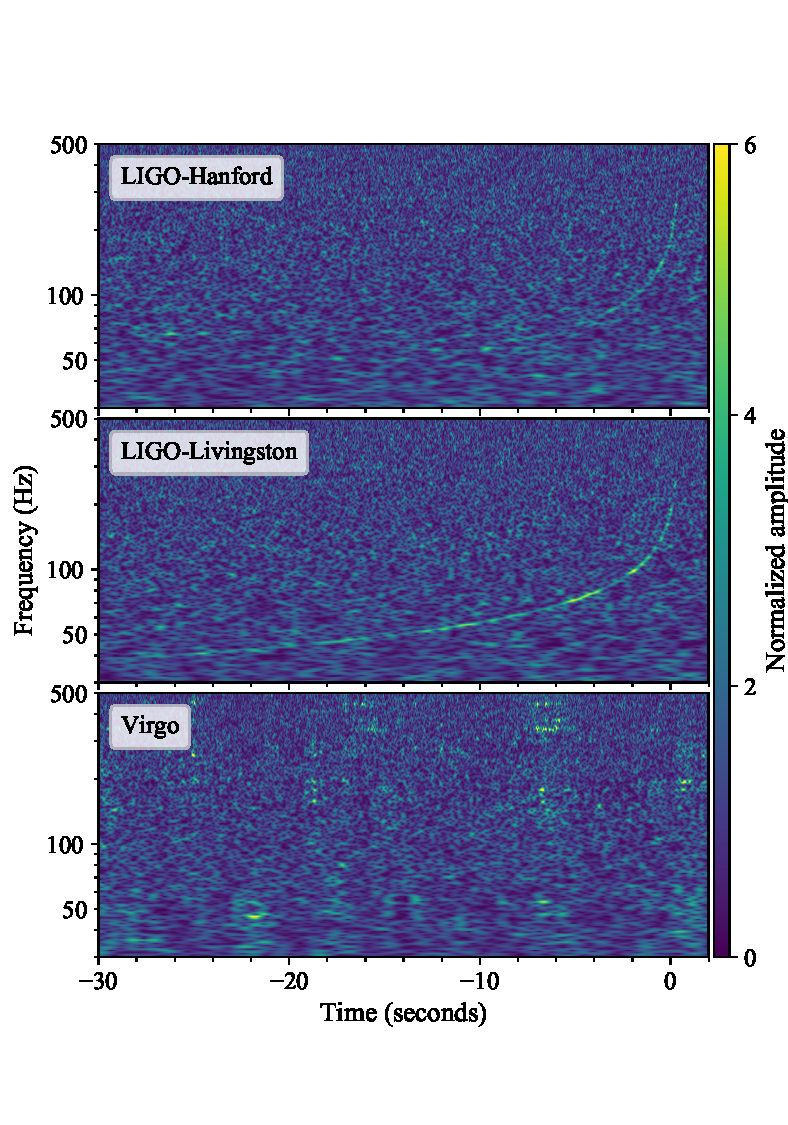
\includegraphics[width=0.85\textwidth]{GW170817.pdf}
\caption{Spectrogram of the strain caused by a binary neutron star merger as seen at the LIGO Hanford Observatory, LIGO Livingston Observatory, and the Virgo Observatory. \cite{GW170817} A clear chirp signal can be seen starting at $\sim$ 40 Hz which rising in both frequency and amplitude.}
\label{GW170817}
\end{center}
\end{figure}
 
 Although binary systems are the topic of choice here, many other systems should theoretically emit gravitational waves. These can range from asymmetric spinning stars and supernova to cosmic strings and density perturbations in the early universe \textbf{cite}. With the measurement of gravitational waves, humankind technologically expand our senses to include the faint vibrations of space-time. This ability has expanded the types of astronomical systems we can study and may one day allow further insight into the beginning of the universe and the nature of gravity.

\section{LIGO}

\subsection{Sensitivity}

The Laser Interferometric Gravitational wave Observatory (LIGO) \textbf{cite} is a pair of 4 km long L-shaped interferometric gravitational wave detectors, one located in Hanford, Washington (LHO) and the other in Livingston, Louisiana. Each observatory is a dual-recycled Fabry-Perot Michelson interferometer which measures the differential strain between its two arms formed by pairs of partially reflective mirrors, also called test masses. 

\begin{figure}%
\begin{center}
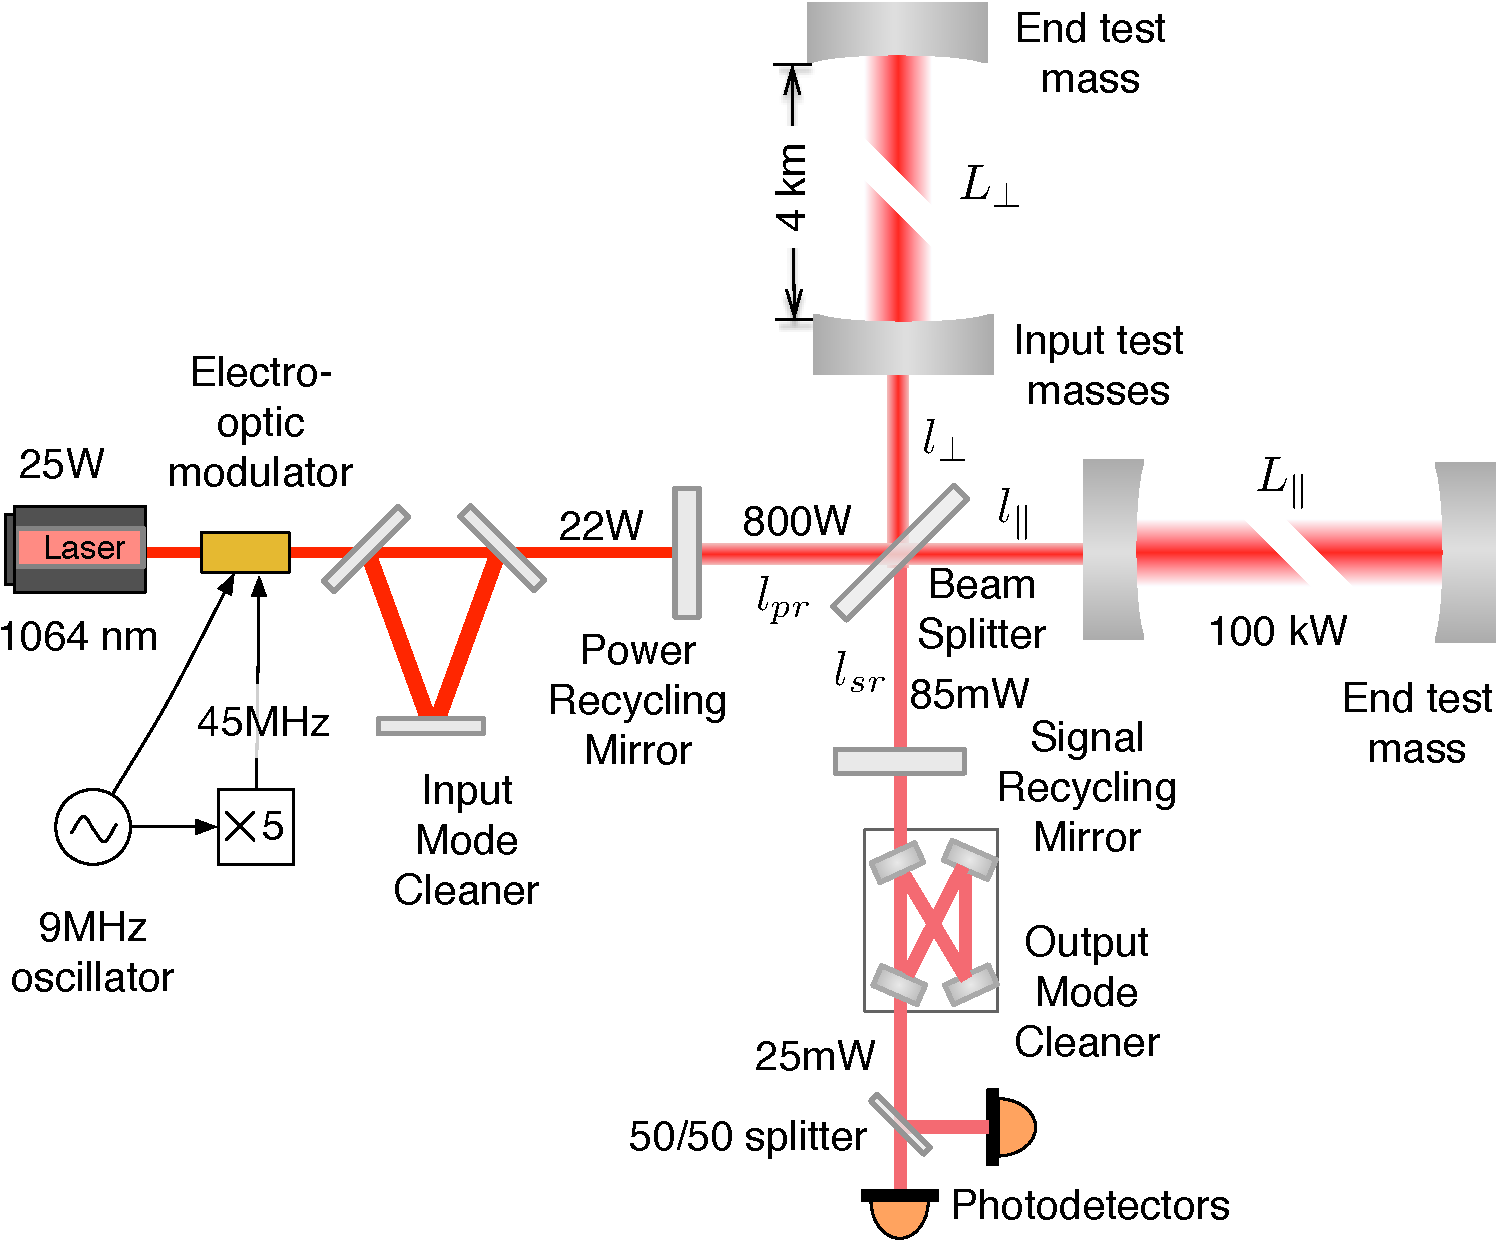
\includegraphics[width=0.85\textwidth]{LIGO_Schematic.pdf}
\caption{\textbf{CHECK COPYRIGHT}}
\label{LIGO_Schematic}
\end{center}
\end{figure}

As a gravitational wave passes the observatory, the arms experience a strains that follow \cite{GWBook}:
\begin{align}
h_{xx}&=h_+\ \big( \cos^2\theta\ \cos^2\phi-\sin^2\phi \big)+2\ h_\times\ \cos \theta\ \sin \phi \cos \phi \\
h_{yy}&=h_+\ \big( \cos^2\theta\ \sin^2\phi-\cos^2\phi \big)-2\ h_\times\ \cos \theta\ \sin \phi \cos \phi \\
\nonumber \\
h&=\frac{1}{2} \big( h_{xx}-h_{yy} \big)=\frac{1}{2}h_+\ \big( 1+\cos^2\theta \big)+ h_\times\ \cos \theta\ \sin 2 \phi 
\end{align}
where $h_{xx}$ and $h_{yy}$ are the strain along the x and y arm respectively, $\theta$ and $\phi$ are the polar and azimuthal angles of the direction of propogation, and $h$ is the differential strain as measured by the observatory. Here the polarizations are defined in the source frame.

The complex series of optics allows the observatory to measure differential strains down to \textbf{$10^{-23}$ at 40 Hz}.  A noise curve for \textbf{some} observatory is shown in Figure \ref{strainNoise} where one can see that the sensitive band of the observatory runs from \textbf{30 Hz up to 16 kHz}. At low frequencies the noise is dominated by residual control noise while at high it is dominated by noise caused by quantum fluctuations.  \textbf{cite}

\textbf{include LIGO strain curve}

\subsection{Events}

With the current sensitivity the primary systems of interest are compact binaries, discussed in Section \ref{CBC}, which merge within the band of interest. A equal mass \textbf{$200\ M_\odot$} binary black hole system would merger at \textbf{11 Hz} while a \textbf{$1.4\ M_\odot$} binary neutron star system mergers at \textbf{1.5 kHz} yet emits appreciably while sweeping through the LIGO band.

During the first and second observing runs of LIGO, ten binary black hole systems and one binary neutron star merger were detected with high significance. \cite{GWTC} The black holes ranged from \textbf{$7\ M_\odot$ to $120\ M_\odot$} and merged at distances from \textbf{100 Mpc to 2 Gpc}. The neutron star binary was composed of a \textbf{$1.2\ M_\odot$ and a $1.4\ M_\odot$} at \textbf{1 Mpc}. These systems are tabulated in Table \ref{gwTable}. \textbf{mention new BNS}

\begin{center}
\begin{tabular}{| c | c | c | c | c | c |}
\hline
Event Name & m1 ($M_\odot$) & m2 ($M_\odot$) & $M_f\ (M_\odot)$ & Distance (Mpc) & z\\
\hline \hline
GW150914 & $35.6^{+4.7}_{-3.1}$ & $30.6^{+3.0}_{-4.4}$ & $63.1^{+3.4}_{-3.0}$ & $440^{+150}_{-170}$ & $0.09^{+0.03}_{-0.03}$\\
\hline
GW151012 & $23.2^{+14.9}_{-5.5}$ & $13.6^{+4.1}_{-4.8}$  & $35.6^{+10.8}_{-3.8}$ & $1080^{+550}_{-490}$& $0.21^{+0.09}_{-0.09}$\\
\hline
GW151226 & $13.7^{+8.8}_{-3.2}$ & $7.7^{+2.2}_{-2.5}$ & $20.5^{+6.4}_{-1.5}$ & $450^{+180}_{-190}$ & $0.09^{+0.04}_{-0.04}$\\
\hline
GW170104 & $30.8^{+7.3}_{-5.6}$ & $20.0^{+4.9}_{-4.6}$ & $48.9^{+5.1}_{-4.0}$ & $990^{+440}_{-430}$ & $0.20^{+0.08}_{-0.08}$\\
\hline
GW170608 & $11.0^{+5.5}_{-1.7}$ & $7.6^{+1.4}_{-2.2}$ & $17.8^{+3.4}_{-0.7}$ & $320^{+120}_{-110}$ & $0.07^{+0.02}_{-0.02}$\\
\hline
GW170729 & $50.2^{+16.2}_{-10.2}$ & $34.0^{+9.1}_{-11.1}$ & $79.5^{+14.7}_{-10.2}$ & $2840^{+1400}_{-1360}$ & $0.49^{+0.19}_{-0.21}$\\
\hline
GW170809 & $35.0^{+8.3}_{-5.9}$ & $23.8^{+5.1}_{-5.2}$ & $56.3^{+5.2}_{-3.8}$ & $1030^{+320}_{-390}$ & $0.20^{+0.05}_{-0.07}$\\
\hline
GW170814 & $30.6^{+5.6}_{-3.0}$ & $25.2^{+2.8}_{-4.0}$ & $53.2^{+3.2}_{-2.4}$ & $600^{+150}_{-220}$ & $0.12^{+0.03}_{-0.04}$\\
\hline
GW170817 & $1.46^{+0.12}_{-0.10}$ & $1.27^{+0.09}_{-0.09}$ & $\le2.8$ & $40^{+7}_{-15}$ & $0.01^{+0.00}_{-0.00}$\\
\hline
GW170818 & $35.4^{+7.5}_{-4.7}$ & $26.7^{+4.3}_{-5.2}$ & $59.4^{+4.9}_{-4.8}$ & $1060^{+420}_{-380}$ & $0.21^{+0.07}_{-0.07}$\\
\hline
GW170823 & $39.5^{+11.2}_{-6.7}$ & $29.0^{+6.7}_{-7.8}$ & $65.4^{+10.1}_{-7.4}$ & $1940^{+970}_{-900}$ & $0.35^{+0.15}_{-0.15}$\\
\hline
\end{tabular}
\label{gwTable}
\end{center}

The ongoing third observing run has had \textbf{\#} significant candidates: \textbf{\#} binary black holes, \textbf{\#} binary neutron stars, and \textbf{\#} black hole neutron star systems. Although these candidates have not been verified to be true gravitational wave events, they show a significant increase in rate of detection due to both the decreased noise and increased duty cycle achieved for the third observing run.

\textbf{what have we learned from these events?}

\section{Seismic Isolation}

\subsection{LIGO Scheme}

To operate interferometric observatories that are sensitive to the strains of space time, one must isolate the instrument from all other sources of differential displacement. As the observatories are located on the surface of the earth, the dominate sources of such noise is due to ambient seismic motion. 

The ambient seismic wave-field is continuously excited across a wide frequency range. Between 50 mHz to 1 Hz the ambient spectrum is dominated by the ``microseism'' which is an always-present feature that is sourced by the earth's oceans. Above 1 Hz, the dominate source of seismic motion at the observatories is due to local instrumentation. Yet even in locations without any anthropogenic sources, the ground moves at some level at these frequencies. Without isolation, this motion would dominate any measurements with the interferometer and, more practically, would disrupt any attempt at operating the interferometer at it's ideal alignment. This ideal alignment is referred to as having the interferometer ``locked''.

The LIGO observatories solve this issue by employing a multi-stage seismic isolation system formed of both passive and active stages. First from the ground is the Hydraulic External Pre-Isolation (HEPI) system which is formed by four hydraulic actuators which give a small amount of passive isolation and low frequency active isolation. Suspended from this is the Internal Seismic Isolation (ISI) system. This is a dual-stage six-degree active isolation and is the primary broad-band isolation. From the second stage of the ISI is hung the quadruple pendulum, at the bottom of which is a test mass. This provide high frequency passive isolation which decreases the motion of the test mass by $1/f^8$, where $f$ is the frequency of the motion.

\textbf{Diagram}

\subsection{Internal Seismic Isolation}

The ISI is comprised of two similar stages each suspended from steel blade springs and wires, the first from HEPI and the second from the first. Each stage is controlled using a set of six magnetic actuators whose signal is comprised of a collection of sensors placed on the stage. The motion of the table is sensed with a series of three-axis seismometers which sense motion with respect to an inertial frame. Two separate models of seismometers are combined to utilized the instrument with the lowest noise in a given frequency band. Above \textbf{3 Hz}, Guralp GS13s are used while between \textbf{100 mHz to 3 Hz} Trillium T240s are implemented. These two sensors are ``blended'' together by sending the T240 through a low pass filter and the GS13 through a high pass. The filtered signals are then added together to form the control signal which is sent to the actuators. 

This is done in all six degrees of freedom by having three independent seismometers of each type located 1 meter apart. The three translational signals are comprised of the average of the corresponding seismometer signals, while the three rotational degrees are sensed by the difference of the seismometer divided by the separation.

\begin{figure}%
\begin{center}
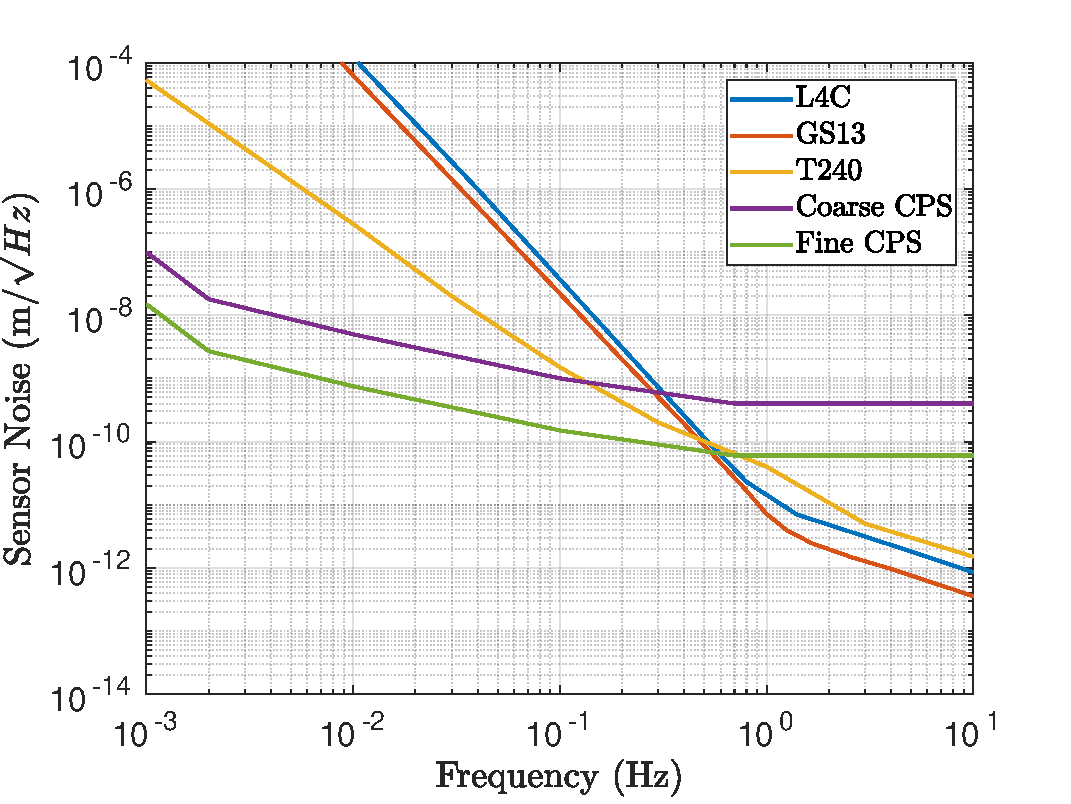
\includegraphics[width=0.85\textwidth]{seismicSensNoise.pdf}
\caption{}
\label{seisNoise}
\end{center}
\end{figure}

Due to the increase in T240 noise below \textbf{100 mHz}, a set of Capacitive Position Sensors (CPS) are deployed which sense the relative motion between either the ground and the first ISI stage or the two stages of the ISI. This is then used as the control signal at low frequencies yielding a control that follows:

\begin{equation}
x_\text{cont}=F_{LP}\ (x_\text{p}-x_\text{g})_\text{,CPS}+F_{BP}\ x_\text{p, T240}+F_{HP}\ x_\text{p, GS13}
\end{equation}

where $x_\text{cont}$ is the control signal, $x_\text{p,i}$ is the platform motion sensed by the respective sensor, $x_\text{g}$ is the ground motion, and $F_\text{LP},\  F_\text{BP},\ F_\text{HP}$ are respectively a low-pass, band-pass, and high-pass filter. When this signal is utilized in feedback, the residual motion of the platform can be approximated by:
\begin{equation}
x_p(f)\approx F_{LP}\ \big(x_g(f)+n_\text{CPS}(f)\big)+F_{BP}\ n_\text{T240}(f)+F_{HP}\ n_\text{GS13}(f)
\end{equation}

where $n_{i}(f)$ is the sensor noise spectrum for the relevant sensor. This approximation ignores tilt to horizontal coupling which is address in Sections \ref{tilt}.

\subsection{Sensor Correction}

The isolation can be improved further with the addition of a three-axis seismometer, in this case a Struckheisen STS-2, placed on the floor of the observatory. This measures the ground motion and can be used to do ``sensor correction''. Sensor correction is the procedure of subtracting the ground contribution of the CPS signal to recover the low frequency platform motion. The CPS signal in this case becomes:
\begin{equation}
x_{CPS}=F_{LP}\ (x_p-x_g)+F_{SC}\ x_g
\end{equation}

where $F_{SC}$ is the ``sensor correction'' filter which has a pass band which over laps the CPS low pass filter. This can be rearranged to give:
\begin{equation}
x_{CPS}=\tilde F_{LP}\ (x_p-x_g)+\tilde F_{HP}\ x_p
\end{equation}

where the tildes denote the relevant combination of $F_{LP}$ and $F_{SC}$. This scheme allows for isolation down to \textbf{10 mHz} and decreases the bleed through of ground motion due to the CPS low-pass filter's finite roll off. Below 10 mHz, both the ground and platform seismometers become dominated by tilt contamination which is addressed in the following Section \ref{tilt}.

\textbf{include ISI performance pre-BRS}

\chapter{1-m Scale Ground Rotation Sensors} \label{BRS_chap}
\section{Ground Tilt}\label{tilt}
\subsection{Tilt Contamination}\label{tiltCon}
\quad At their core, seismometers are low frequency spring-mass system which measure the difference in motion between the casing and the device's proof mass. Above the resonant frequency of the spring-mass system, this allows for accurate measurements of the motion, in reference to an inertial frame, of any object that the casing is rigidly connected to, be it the ground or a suspended table. Over the past \textbf{some time} this technology has produced devices that are sensitive to \textbf{number and range}. However, these systems are fundamentally susceptible to any stray forces acting on the proof mass.

Of interest here is the contamination due to the rotation of the device within a external gravitational field, namely the field caused by the earth. The rotation in respect to a fixed gravitational force will be referred to as tilt.\footnote{Although a subtle difference, the distinction would be of great consequences if the local gravitational field was varying rapidly. In that case the sensors described in Sections \ref{BRSSec} and \ref{cBRSSec} would be of little use as they are rotational sensors not tilt sensors.} From the proof mass's frame, a tilt is equivalent to a rotation of the gravitational force. This yields a horizontal acceleration of the proof mass of:
\[ a=g \sin(\theta)\]
where $g$ is the gravitational acceleration on the surface of the earth and $\theta$ is the angle that the device is rotated. This acceleration adds a second term to the seismometer's output shown below for small angles and in the Fourier domain:
\[\tilde{x}_{seis}(\omega)=\tilde{x}_{trans}(\omega)+\frac{g}{\omega^2}\tilde{\theta}(\omega)\]
where $x_{seis}$ is the seismometer's output, $x_{trans}$ is the translational motion of the device, and $\omega$ is the frequency. 

With this additional contribution, it becomes immediately clear that, for a given amplitude of tilt, the contamination term contributes more at lower frequencies and readily dominates the translational signal. In the context of the ground seismometers at the observatory, the tilt signal swamps the translational component below $\sim$ 100 mHz. Above which the seismometer signal is dominate by the ever-present oceanic microseism which is driven by low frequency pressure waves within the ocean and their interaction with the shoreline. \textbf{CITE} This can be seen in Figure \ref{wind} which shows an amplitude spectral density of a ground seismometer at LHO during both low and high wind conditions.

\begin{figure}%
\begin{center}
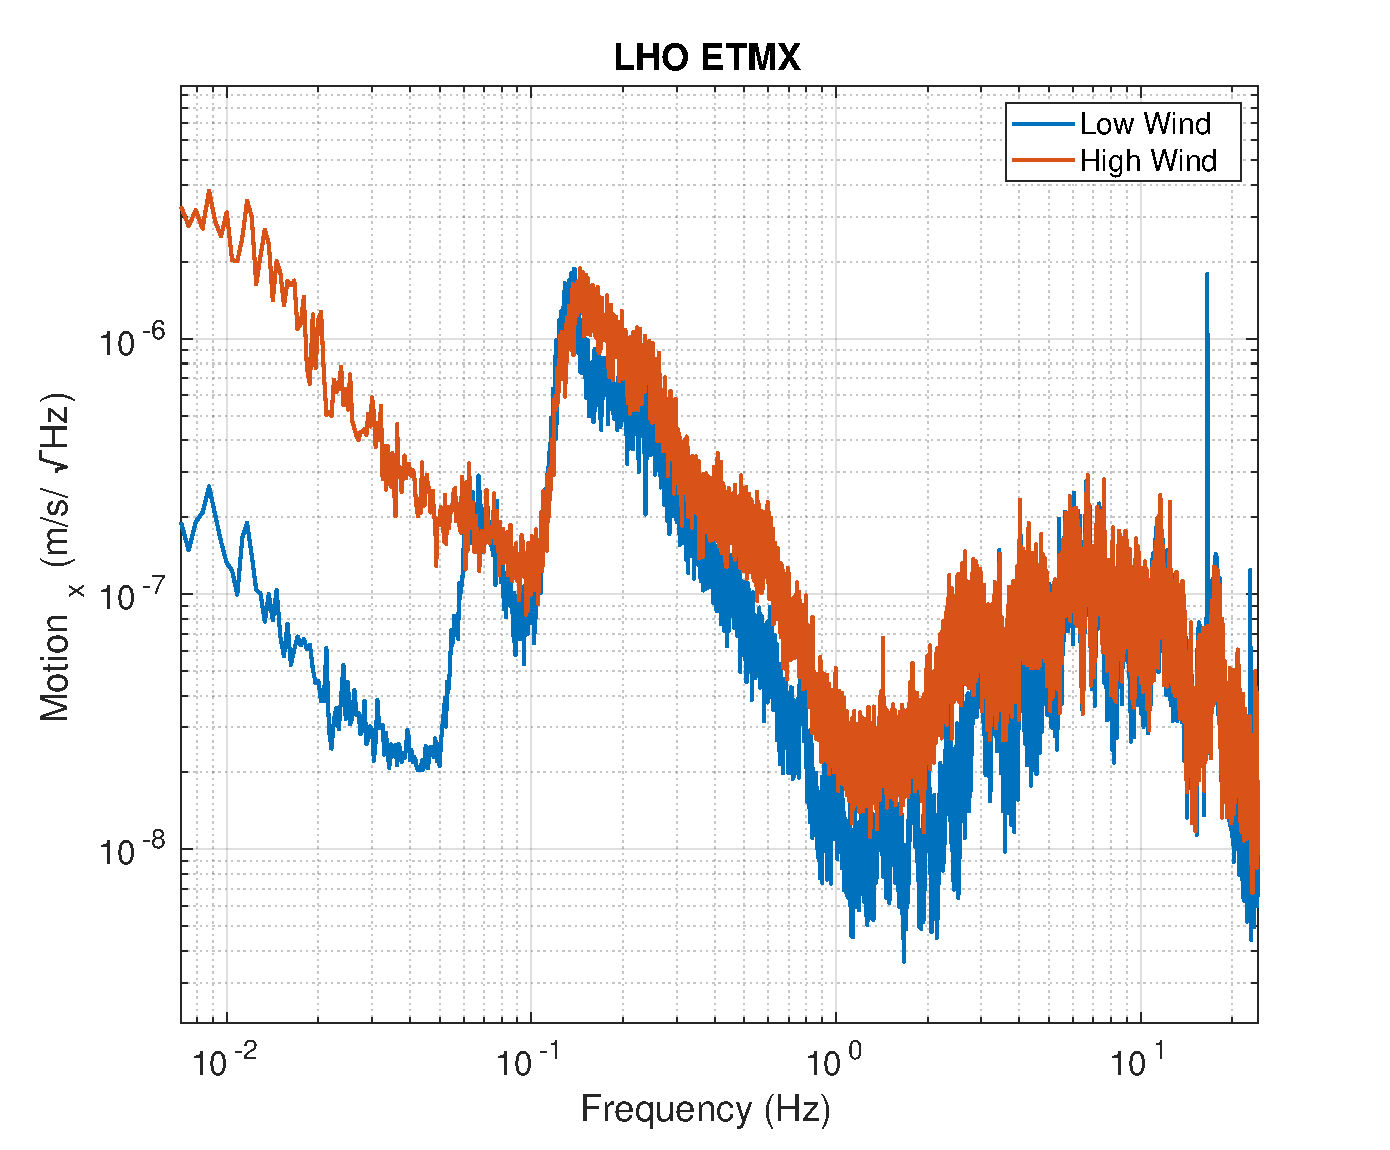
\includegraphics[width=0.75\textwidth]{windComp.pdf}
\caption{Ground motion spectra recorded at the X end station of the Hanford Observatory during low and high winds. Below 100 mHz, wind driven tilts become dominate during high winds. From 100 mHz to 1 Hz the spectra are dominated by the oceanic microseism while above 1 Hz the seismic motion is sourced by local athropogenic activity.}
\label{wind}
\end{center}
\end{figure}

The dominate driver of ground tilts at the observatories is wind acting on the walls of the building. Although one would naiively assume that the wind would rigidly rotate the building, it was found that the true mechanism is differential pressure acting on the walls to deform the building's concrete slab. \textbf{cite?} This increased the noise in the ground seimometer used in sensor correction which limited the performance of the seismic isolation during high winds. The primary consequence of this excess is that the observatory could not operate during high wind speeds.

\subsection{Sensor Correction with Tilt Subtraction}

\quad There are a few different scheme to combat such a contamination. The most straight forward is to decrease the effect of wind by designing buildings which interact with the wind less or by installing wind blocks such as wind fences or earth burms. Both of these options require significant construction and, for the case of LIGO, tilt contamination was not known to be a problem when the observatories were designed. Another option is to build seismometers that are suspended in such a way that they do not experience tilts. This is an active area of research and may yield tilt-free seismometers. \textbf{cite}

The scheme that will be described here is to measure the tilt with an independent rotation sensor and subtract the wind-driven contribution. This would then yield a channel of the following form:
\begin{align}
x_{seis}(\omega)=x_{trans}(\omega)+&\frac{g}{\omega^2}\theta(\omega)\\
-&\frac{g}{\omega^2}\theta_{meas}(\omega)
\end{align}

where $\theta_{meas}$ is the tilt seen by the rotation sensor. Given a subtraction factor of $\alpha$ between the tilt component of the seismometer and rotation sensors this yields the following: \textbf{CHECK math}

\[x_{seis}(\omega)=x_{trans}(\omega)+\frac{g}{\omega^2}(1-\alpha)\theta(\omega)\]

Current installations have yielded an $\alpha\sim 0.9$. This is then a low tilt channel which can be used within the LIGO seismic isolation system. As this decreases noise primarily at low frequencies, the feedback filters deployed within the isolation system can be tuned to cross over at lower frequency away from the mircoseism. At the cross over frequency, the filters have both large gain and phase changes which decrease performance. Moving this cross-over away from the microseism decreases the effect of these properties and allows for isolation to lower frequencies.

\section{Beam Rotation Sensors} \label{BRSSec}
\subsection{Mechanical System}

\quad The Beam Rotation Sensor (BRS) is a beam-balance comprised of a 1-m long beam hung from two 10-15 $\mu$m thick beryllium-copper flexures. Figure \ref{BRSImage} shows a CAD model of the beam-balance. 

\begin{figure}
\begin{center} 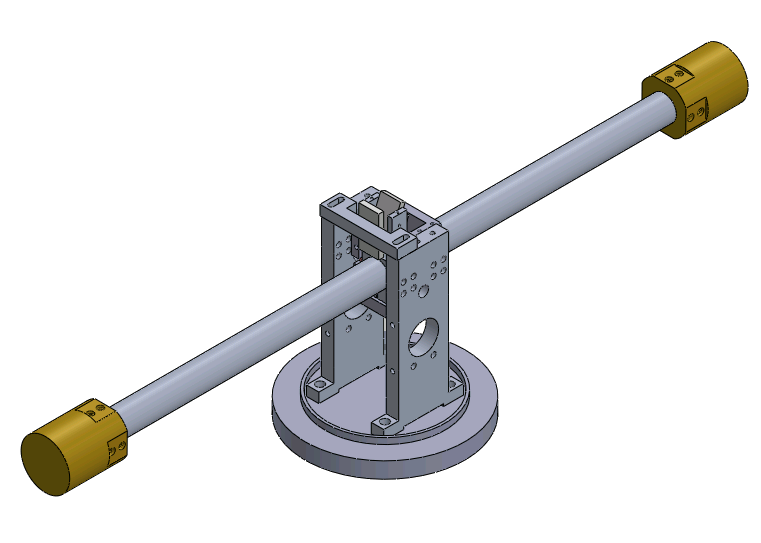
\includegraphics[width=0.75\textwidth]{BRSIso.png}
\caption{CAD rendering of the Beam Rotation Sensor with the vacuum and optical readout systems omitted. The bem with its two brass end masses can be seen through the thermal shielding, shown here as transparent. }
\end{center}
\end{figure} 
\begin{figure}
\begin{center} 
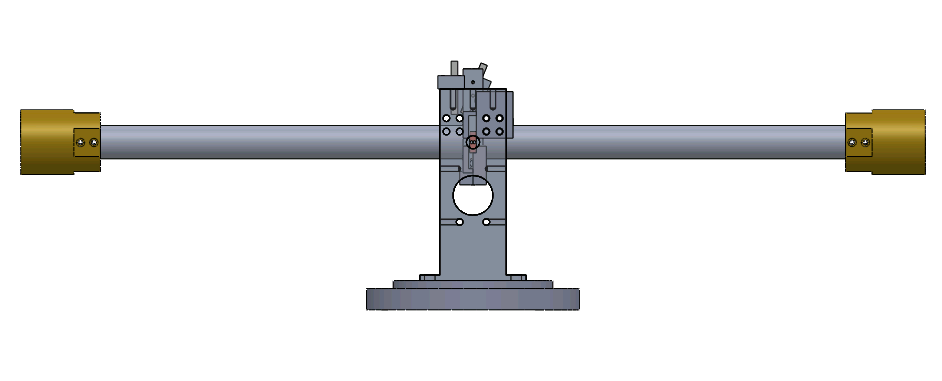
\includegraphics[width=\textwidth]{BRSFront.png}
\end{center}
\caption{CAD rendering of the Beam Rotation Sensor with the vacuum and optical readout systems omitted. The bem with its two brass end masses can be seen through the thermal shielding, shown here as transparent. }
\label{BRSImage}
\end{figure}

\begin{figure}
\begin{center} 
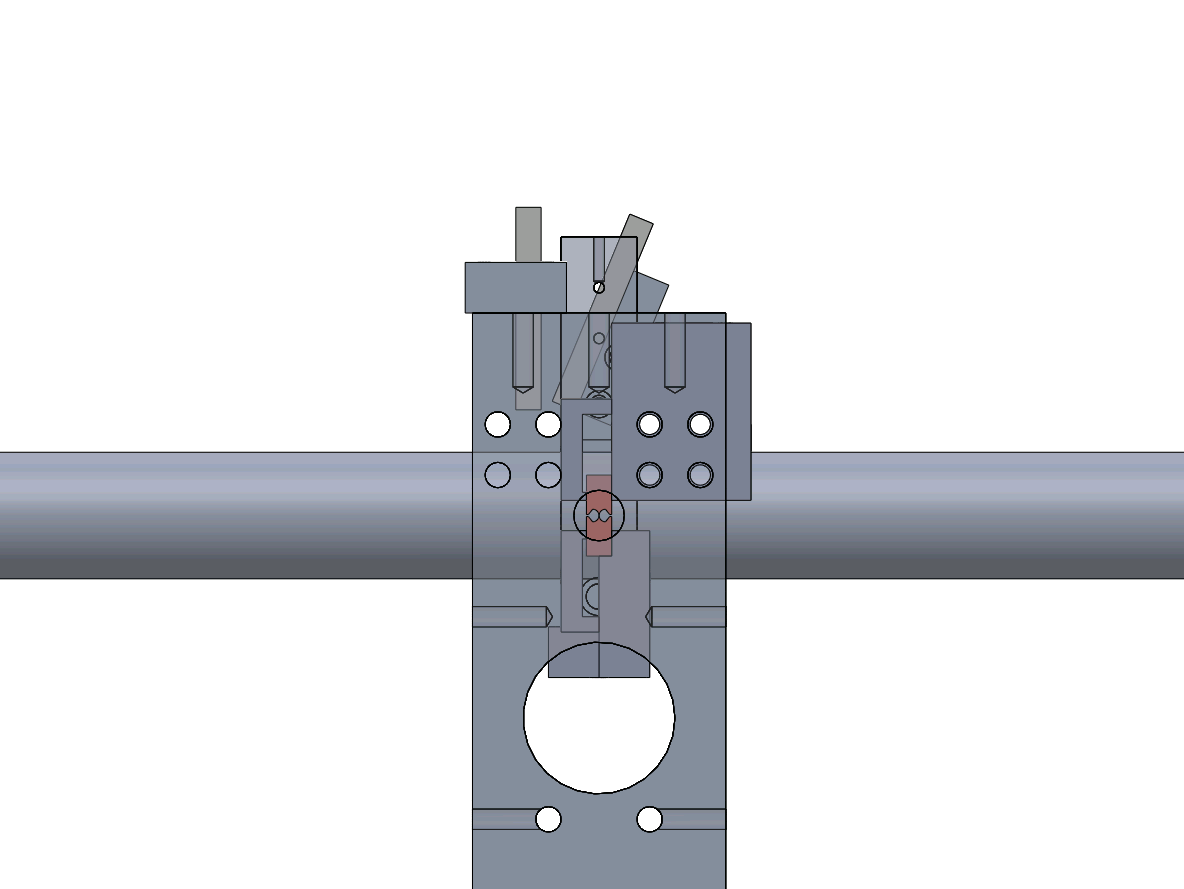
\includegraphics[width=\textwidth]{BRSFrontDetail.png}
\end{center}
\caption{CAD rendering of the Beam Rotation Sensor with the vacuum and optical readout systems omitted. The bem with its two brass end masses can be seen through the thermal shielding, shown here as transparent. }
\end{figure}


This design makes the beam stiff in all degrees of freedom other than rotations around the horizontal axis which intersects the two flexure pivot points. This forms a system consisting of two elementary subsystems: a rotational spring-mass system formed by the stiffness of the flexures, and a simple pendulum due to the offset of the pivot point and the center of mass. This is then described by the following equation of motion: \cite{venk2014}

\begin{equation}
I \ddot{\theta}+ \gamma \dot{\theta}+\kappa (1+ \frac{i}{Q})(\theta-\theta_p)+M g \delta \theta +M \delta \ddot{x_p}=\tau_{ex} \label{eom}
\end{equation}

where $\theta$ and $\theta_p$ are, respectively, the angle of beam and the platform with respect to gravitational vertical, $\tau_{ex}$ is the sum of all exterior torques, $I$ is the moment of inertia, $Q$ is the intrinsic quality factor, $\gamma$ is the velocity damping factor, $\kappa$ is the spring constant of the flexures, $M$ is the mass of the balance, $g$ is the gravitational acceleration, $\delta$ is the vertical distance from the center of mass and the pivot point, and $x_p$ is the translation of the platform. Equation \ref{eom} can be rearranged to yield:

\begin{equation}
\theta = -\frac{\tau_{ex}+\omega^2 M \delta x_p+\kappa (1+i/Q) \theta_p}{I\omega^2-i \gamma \omega -i \kappa /Q-\kappa -Mg\delta}
\end{equation}

where $\omega$ is the frequency of motion. For the BRSs, the quantity of interest is not the angle of the beam but the difference in angle between the beam and the platform. Thus the angle that readout records follows:

\begin{align}
\theta_a &=\theta-\theta_p\\
&= -\frac{\tau_{ex}+\omega^2 M \delta x_p+\kappa (I\omega^2-i\gamma \omega -Mg\delta) \theta_p}{I\omega^2-i \gamma \omega -i \kappa /Q-\kappa -Mg\delta}
\end{align}
where $\theta_a$ is the recorded angle. This equation can be broken up into three distinct terms: the angular motion due to external torques, $\theta_\tau$, due to translational coupling, $\theta_x$, and due to rotation of the platform, $\theta_s$.
\begin{align}
&\theta_a =\theta_\tau+\theta_x+\theta_{s}\\
&\theta_\tau= -\frac{\tau_{ex}}{I}\frac{1}{\omega^2-i (\omega_0 \omega/q+\omega_0^2/Q)-(\omega_0^2+\omega_g^2)}\\
&\theta_x= -x_p\frac{M\delta}{I} \frac{\omega^2}{\omega^2-i (\omega_0 \omega/q+\omega_0^2/Q)-(\omega_0^2+\omega_g^2)}\\
&\theta_{s}= -\theta_p\frac{\omega^2-i\omega_0 \omega/q-\omega_g^2}{\omega^2-i (\omega_0 \omega/q+\omega_0^2/Q)-(\omega_0^2+\omega_g^2)}\label{theta_s}
\end{align}

Where $\omega_0=\sqrt{k/I}$ is the resonant frequency, $\omega_g=\sqrt{M g \delta/I}$, and $q$ is the quality factor due to velocity damping. These equations illuminate the fact that the beam has a resonance at $\omega=\sqrt{\omega_0^2+\omega_g^2}$ and $\theta_s$ has a zero at $\omega=\omega_g$. 

To allow for high fidelity rotation sensing, the translational coupling must be negliable at the frequencies of interest. To achieve this, $\delta$ must be tuned close to zero. This is achieved firstly through the design of the beam's suspension which places the center of mass close to the pivot point. Fine adjustments are them made by adding mass to the beam above or below the pivot. These adjustments are guided by measurements of the zero in the $\theta_s$ transfer function, Equation \ref{theta_s}, at $\omega=\omega_g$. Differing amounts of tuning were achieved for each device described Section \ref{results} due to scheduling constraints. The lowest translation coupling was achieved at the LHO End-Y BRS which had a $\delta<0.5\ \mu$m yielding a translational coupling of $<10^{-6}$ rad/m.


\subsection{Multi-Slit Autocollimator Readout}

\quad Optical levers are simple optical angular readouts which exploit the law of reflection to measure angular deflections of a mirror by observing the displacement of a reflected beam. The angle of the mirror is then described as:
\begin{equation}
\theta_{\text{mirror}}=\frac{x_{\text{reflected}}}{2d}
\end{equation}
where $\theta_\text{mirror}$ is the angle of the mirror, $x_\text{reflected}$ is the displacement of the reflected beam, and $d$ is the distance between the optical system and the mirror. This allows one to increase the precious of the angular measurements arbitrarily by increasing $d$. However, with this comes a few disadvantages. One the effective gain of the sensor depends of the $d$ which may not be well known. Additionally, the system is sensitive to changes in $d$. 

An autocollimator adds a lens located one focal length from light source and the screen, shown in Figure \textbf{number}. This effectively replace the distance dependence with the focal length of the lens which allows the system to be only sensitive, to first order, to the angular motion of the mirror.

\begin{figure}%
\begin{center}
 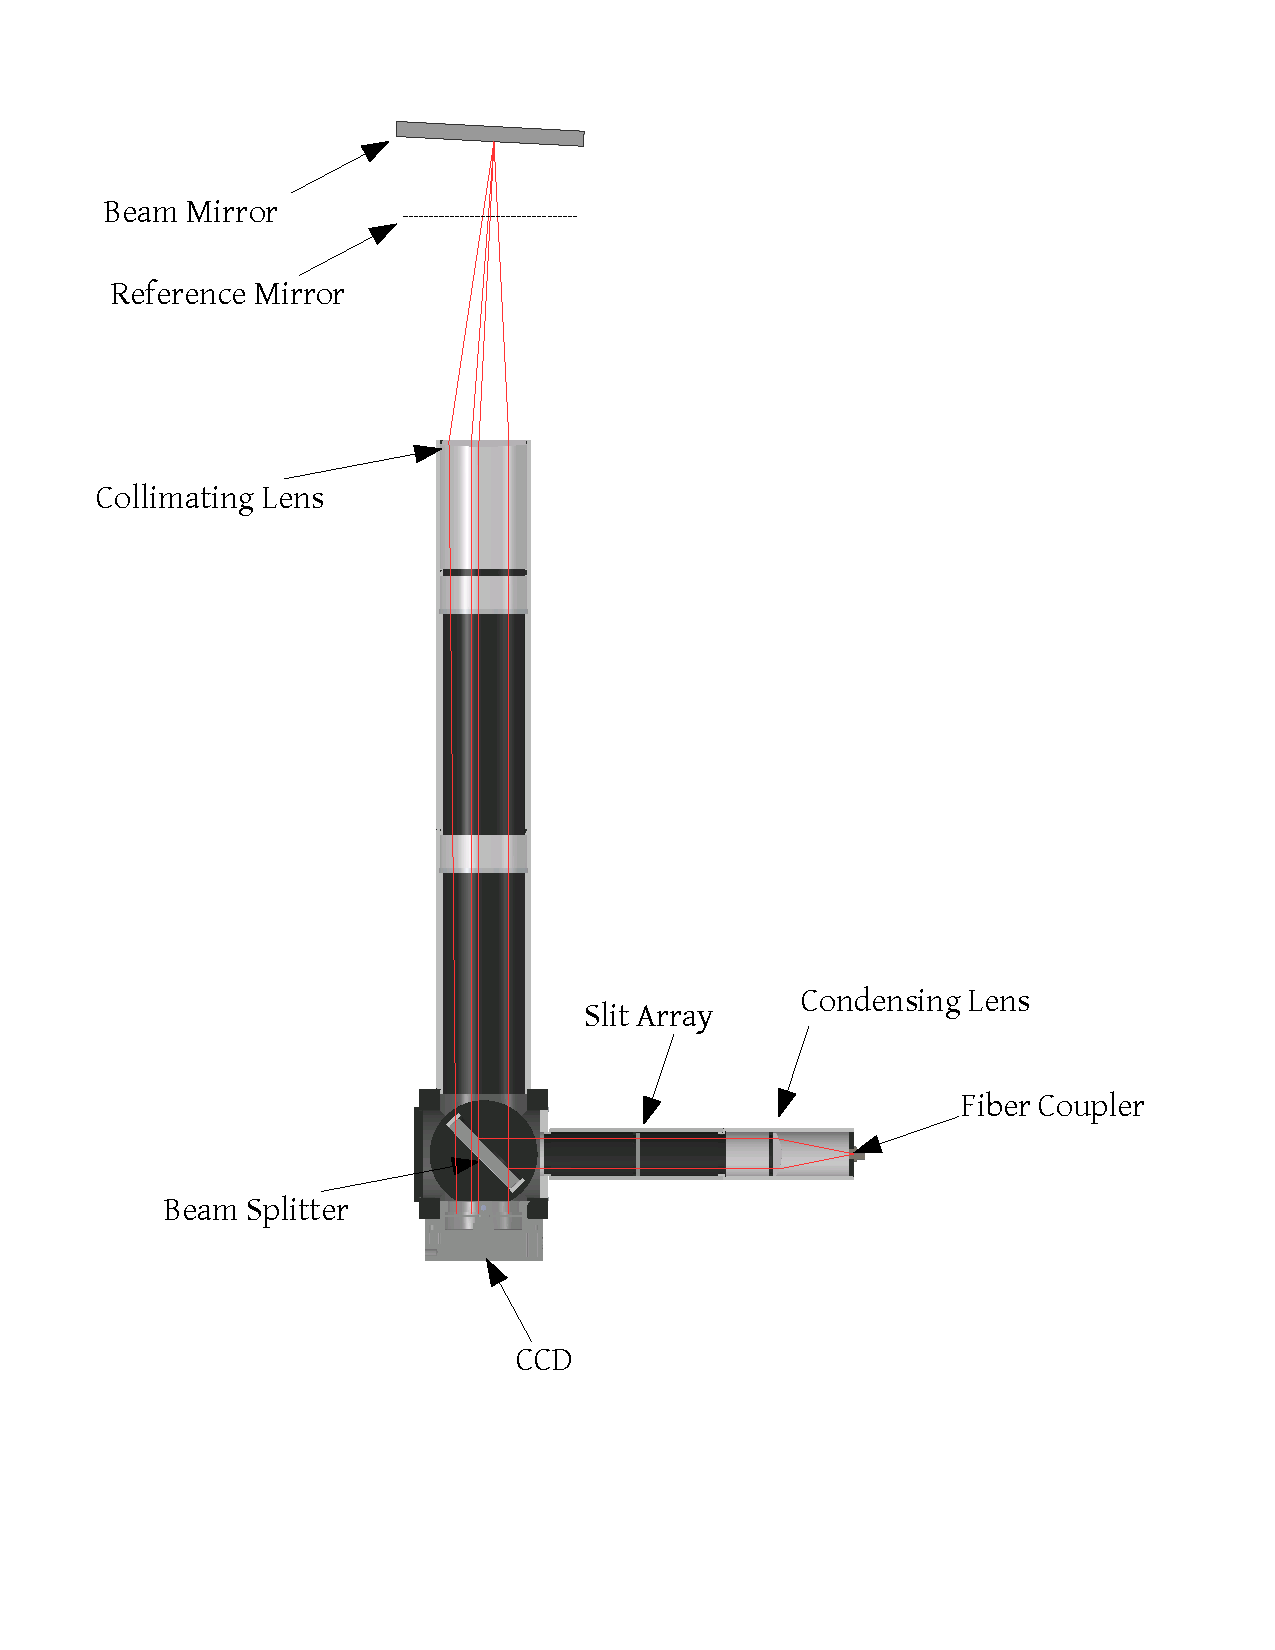
\includegraphics[width=\textwidth]{Autocollimator.pdf}
\caption{Schematic of autocollimator.}
\label{ACFig}
\end{center}
\end{figure}

To improve upon this further, a partially reflective mirror can be placed in between the optical system and the main mirror to act as a reference and allows for the subtraction of any motion of the optical system with respect to the main mirror. This yield a angular readout described by:
\begin{equation}
\theta_{\text{mirror}}=\frac{x_{\text{main}}-x_{\text{reference}}}{2f}
\label{ACEq}
\end{equation}

where $f$ is the focal length of the lens and $x_\text{reference}$ is the beam spot from the reference mirror.

\begin{center}
\begin{tabular}{| c | c |}
\hline
Parameter & Value\\
\hline \hline
CCD & Balser Racer raL4096-24 gm\\
Pixel Number & 4096\\
Pixel Size & 7 $\mu$m $\times$  $\mu$m\\
Pixel Depth & 12 bits\\
Light Source & Fiber coupled LED\\
Wavelength & 455 nm\\
Condensing lens focus & 50 mm\\
Collimating lens focus & 500 mm\\
Number of slits & 38\\
Slit size & $\sim$0.127 mm\\
\hline
\end{tabular}
\label{ACTable}
\end{center}

An increase in sensitivity can be made by employing a multi-slit autocollimator \cite{MSA}. Such a systems are deployed as the angular readouts for the BRSs. This consists of an autocollimator with the light source replaced by a illuminated photomask of a number of thin slits. The pattern is then reflected off a set of reference and main mirror and imaged by a line CCD camera. These images are then analyzed to measure the distance between them thus yielding a measurement of angle. For the BRSs, this image analysis is achieved using bespoke software written in C\# which can be found at www.github.com/mpross/BRSReadout

To extract the distance between the patterns, the image goes through a series of steps which take it from a vector of pixel intensities to a single angular output. When the software begins, the first frame that is captured is saved. All future frames are split into two, with one part representing the reference mirror and the other the main mirror. The cross correlation is then taken between each part and it's matching section of the first frame. This gives a curve who's maximum is located at the pixel number corresponding to separation between the pattern in the current frame and the first frame, which can be seen in Figure \textbf{number}. The points of this curve that are near the maximum are then fit to a Gaussian which allows for the extraction of the location of the peak with sub-pixel resolution. This is done for each pattern separately after which the difference between the reference pattern location and the main pattern location is taken. The difference is then proportional to the change in angle between the casing and the beam following Equation \ref{ACEq}.

Compared to previous image analysis algorithms \cite{MSAPaper}, this algorithm is more computationally efficient while also being less susceptible to variations in the pattern image due to dust particulate, incorrect focusing, or beam clipping. A sensitivity of \textbf{$\sim$ 0.1 nrad$/\sqrt{\text{Hz}}$} was achieved with this autocollimator design and image analysis algorithm.

\subsection{Controls}

\quad As the BRSs are installed in active lab spaces, anthropogenic actively and environmental disturbances regularly apply torques on the beam-balance, either through mechanical coupling through the flexures or gravitational coupling with the end masses. These can then cause the motion at the resonant frequency to rise to undesirable amplitudes. As the beam motion increases so does the noise. Additionally, some disturbances can be large enough to cause the amplitude to exceed the dynamic range of the autocollimator readout system.

The alleviate this issue, capacitor plates are installed underneath each end of the beam-balance to act as actuators. The force between the two capacitor plates follows the following: 
\begin{equation}
F=\frac{\epsilon A V^2}{2d^2} \label{cap}
\end{equation}
where $\epsilon$ is the permittivity of the material between the plates, $A$ is the area of the plate, $V$ is the voltage applied to the plates, and $d$ is the distance between the plates. The plate under the beam is connected to a DAC while the beam is grounded which allows for a controlled actuation torque to be applied to the beam. 

The control scheme that was adopted was one in which the feedback signal that is sent to the capacitors is the angular velocity of the beam band passed between 2 mHz and 20 mHz to include only motion at frequencies near the resonance. The feedback is additionally applied with low gain so that the feedback only adds loss to the system as compared to locking the system in a strong feedback loop where all of the motion is absorbed into the control system. This is then implemented with two gain stages, a ``low amplitude'' stage, which is always on and yields a Q of 10-15, and a ``high amplitude'' stage, which is triggered if the amplitude rises above a threshold that is set based on the behavior of the given device and gives a Q of \textbf{number}.

\subsection{Noise Performance}

In addition to the 0.1 nrad/$\sqrt{\text{Hz}}$ white noise of the autocollimator readout, these devices suffer from various mechanical noise sources, namely noise due to temperature variations and due to the thermal motion of the flexures.

Although the exact physical mechanism is unknown at this juncture, it has been observed that variations in the exterior temperature cause shifts in the balance's equilibrium position. Furthermore, temperature gradients across the instrument emanating from unbalanced heat sources and air currents have been seen to cause time varying noise. To alleviate this issue the instrument's vacuum chamber and optics are wrapped in multiple alternating layers of packing foam and aluminum foil. The entire apparatus is then placed inside a large double walled insulation box to further decrease any temperature variations. This eliminates this as a dominate noise source unless the room in which the instrument is housed undergoes large temperature variations.

More fundamental is the noise due to the thermal vibrations of the flexure. At non-zero temperature, a portion of the thermal energy of the flexures is stored in the vibrational modes. This causes a fundamental stochastic noise floor that follows\cite{thermal}:

\begin{equation}
\tilde\theta_T(\omega)=\sqrt{\frac{4 k_B T \omega_0^2}{I \omega Q\big((\omega^2-\omega_0^2)+\omega_0^4/Q^2\big)}}
\end{equation}

Since this noise source enters as a torque on the beam-balance, it is filtered by the harmonic response making it fall as $1/f^2$ above the resonant frequency. To limit the influence on the performance of the device, the resonant frequency of the spring-mass system is pushed to the lowest frequency that is mechanically feasible. This is the fundamental noise of the instrument and thus is independent of readout and environmental effects.


 \textbf{post inversion thermal noise}
 
 One further noise source comes from voltage noise on the capacitive actuators. The force follows Equation \ref{cap} and can be shown to be sub dominate\textbf{show this}.
 
 \begin{figure}%
\begin{center}
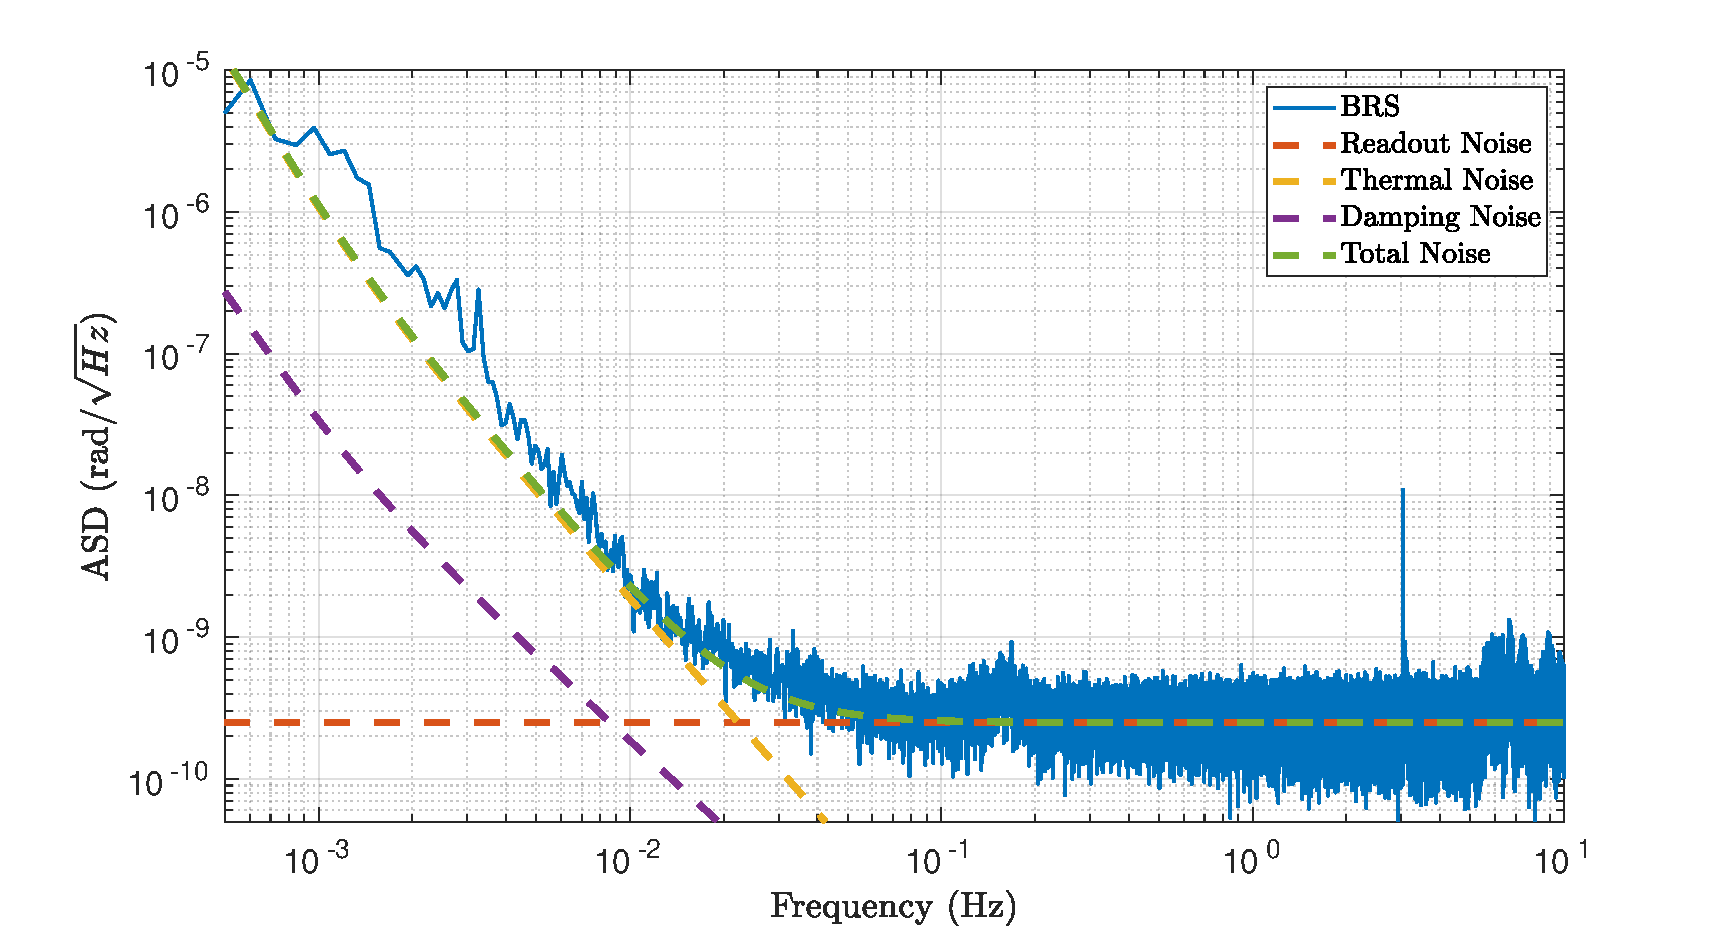
\includegraphics[width=\textwidth]{BRSNoiseBudget2.pdf}
\caption{Noise budge for the Beam Rotation Sensors where the blue curve shows the performance at a quiet time, in red is the motion of the reference mirror which can be regarded as an estimate of the readout noise, yellow shows an estimate of the thermal noise, purple shows the noise from the capacitive actuators, and green shows the sum of all known noise sources.}
\label{noise}
\end{center}
\end{figure}

 The noise budget for a BRS is shown in Figure \ref{noise} which shows that the device is readout dominated above $\sim$20 mHz and below is dominated by thermal noise. An excess in the measured noise can be seen below 3 mHz which is believed to be due to residual temperature noise. Respectively at 150 mHz, 3 Hz, and 6 Hz the rotational microseism, torsion mode of the beam-balance, and motion due to nearby instrumentation can be seen above the predicted noise sources.

\section{Results}\label{results}
\subsection{Hanford Installation} \label{BRS_Hanford}

\quad Between LIGO's first (O1) and second (O2) observing runs, two BRSs were installed at the LIGO Hanford Observatory (LHO), one at each end station correcting the translations along their respective arm. Although one would expect that the corner station seismometers would also need to be corrected, a location was found within the corner station building which exhibited low tilt. \textbf{cite} This is thought to be due to the distance between this location and the walls of the building. As such no BRS was necessary to achieve low tilt contamination.

\begin{figure}%
\begin{center}
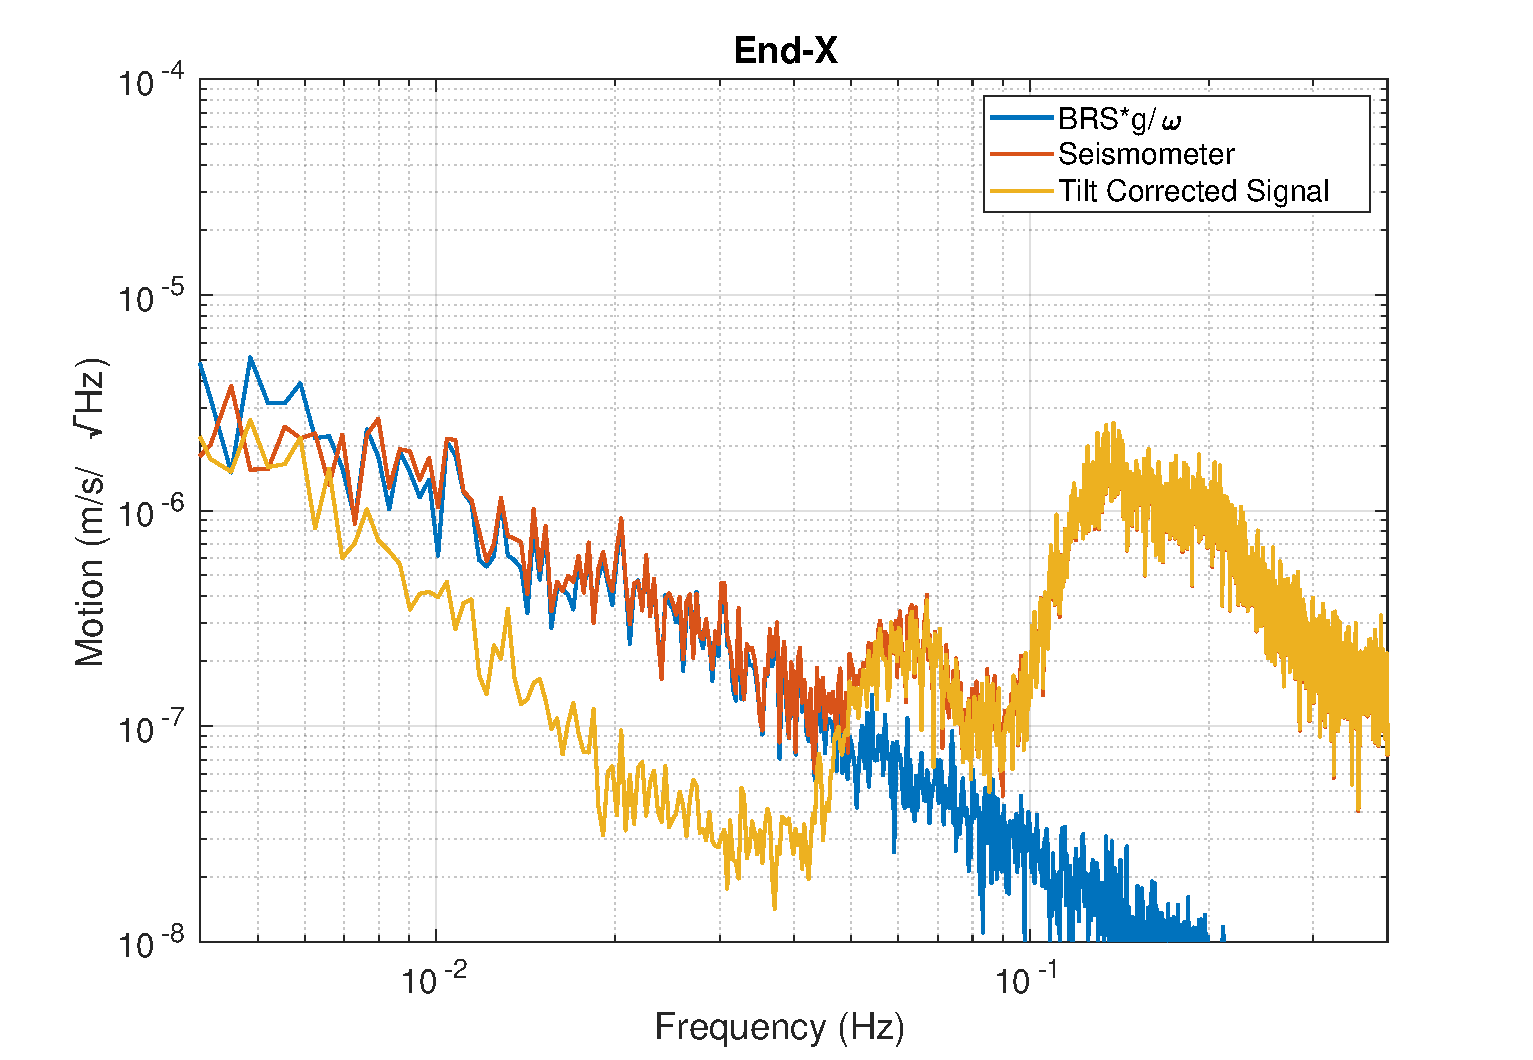
\includegraphics[width=\textwidth]{HSubtractionETMX.pdf}
\caption{Representative amplitude spectral density showing the tilt subtraction during windy conditions achieved at End-X of LHO where blue is the BRS signal multiplied by $g/\omega$, read is the raw seismometer signal, and yellow is the tilt corrected signal. Similar perform has been achieved by all of the deployed BRSs.}
\label{sub}
\end{center}
\end{figure}

The tilt subtraction performance achieved with these devices can be seen in Figure \ref{sub} where it is evident that the system achieves tilt subtraction from around 6 mHz to 50 mHz. Above 50 mHz the seismometer signal is dominated by the oceanic microseism and the tilt contribution is negligible. Below 6 mHz, the BRS signal becomes overwhelmed by instrumental noise. This performance can also be seen in Figure \ref{subTime} which shows a example time series of the tilt subtraction. 

\begin{figure}%
\begin{center}
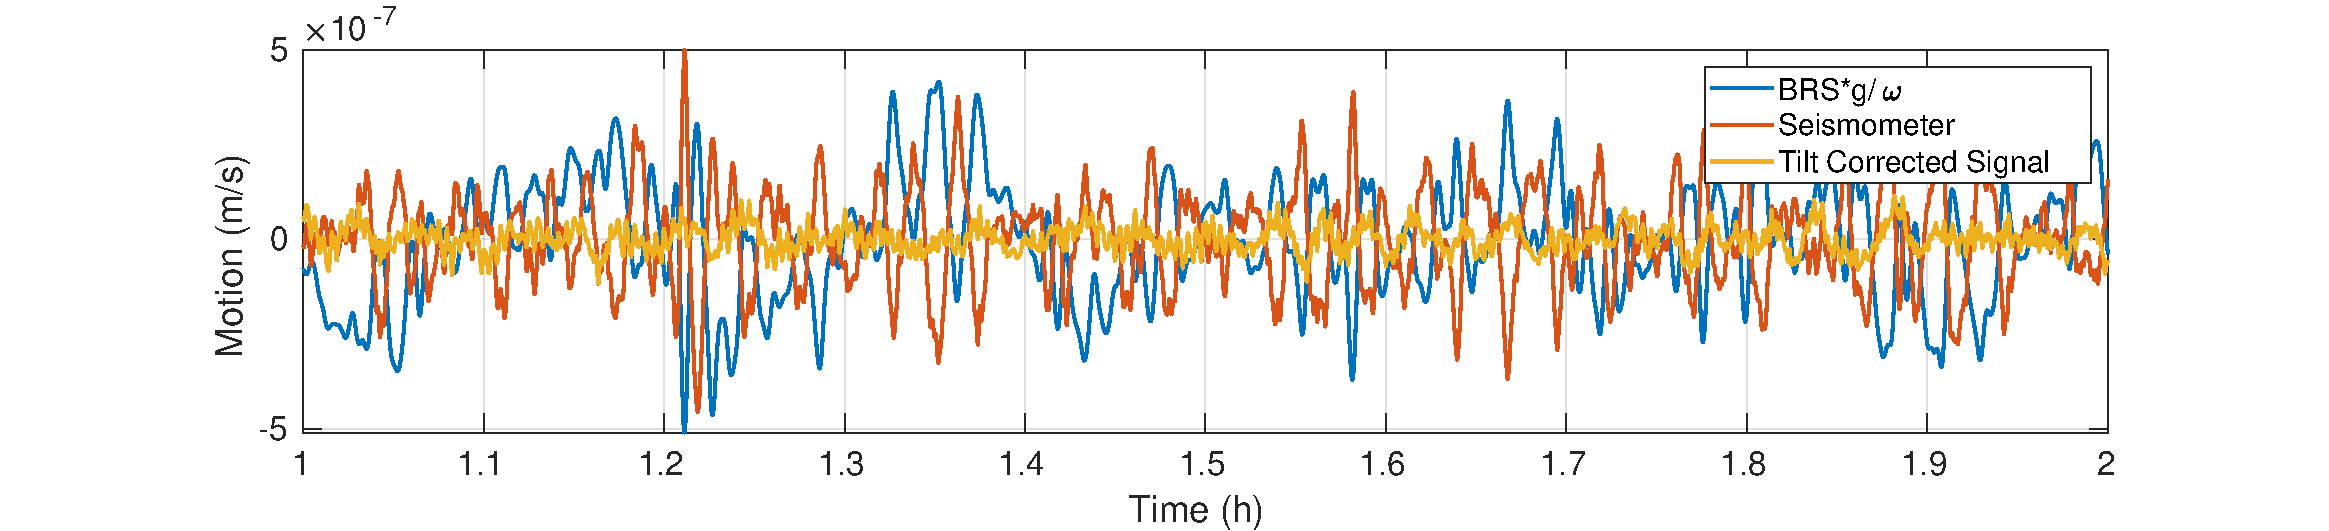
\includegraphics[width=\textwidth]{TiltCorrTime.pdf}
\caption{Time series showing the tilt subtraction at End-X of LHO where blue is the BRS signal multiplied by $g/\omega$, read is the raw seismometer signal, and yellow is the tilt corrected signal. As can be seen, the tilt subtraction removes a collection of transients, likely due to the gusts of wind.}
\label{subTime}
\end{center}
\end{figure}

This tilt subtracted channel was then used as the ground signal for the isolation's sensor correction instead of the raw seismometer. Along with the use of the low tilt seismometer for the corner station, the addition of the BRSs in the seismic control scheme yielded significant improvements in the ability to lock the interferometer at increased wind speeds which can be seen in Figure \ref{O2}

\textbf{List BRS parameters}


\subsection{Livingston Installation}

\quad After the success of the Hanford BRS installation, four devices were installed at the LIGO Livingston Observatory (LLO) between the second and third (O3) observing runs. Due to differences in the size and shape of the corner station building at LLO, a low tilt location was not found. Thus two BRSs were installed located near the two input test masses (ITM) along with one at each end station correcting the seismometer signal oriented along their respective arms. 

All four were implemented in a similar fashion as the Hanford devices. \textbf{More}

\subsection{Ground Tilt Model}

As mentioned in Section \ref{}, the primary driver of ground tilts at the observatories is wind acting on the building's walls. This deforms the concrete floor in a non-trivial manner. Thus modeling the ground tilt spectrum for a given wind speed from first principals is intractable. However, with the collection of observations made by the BRSs installed at the sites, an empirical model can be constructed.

To achieve this, hour long spectra of the BRS at the End-X of LHO were sorted into a collection of bins depending on the average wind speed measured during that hour. Each bin was then averaged to yield a representative spectrum for each wind speed. This was then fit to an empirically determined model, Equation \ref{TiltModelEq}, containing two terms: the first constituting the broad behavior of the spectrum and a second which enhances the high frequency motion at high wind speeds. The parameters of this were then fit vs wind speed to yield a tilt spectrum vs wind speed model. 

\begin{align}
\theta&=\frac{x_1}{f^{2/3}(1+f/f_1)} +\frac{x_2}{1+(f/f_2)^3}\label{TiltModelEq}\\
\nonumber \\ 
f_1&=0.2\ \text{Hz}\nonumber \\
f_2&=(0.1\ s -0.25)\ \text{Hz}\ \text{if }s>0\text{ else }f_2=0\nonumber \\
x_1&=(1.4\times10^{-11}\ s^2+5.7\times10^{-11}\ s+6.4\times10^{-11})\ \text{rad}\nonumber \\
x_2&=(1.8\times10^{-10}\ s^2-7.6\times10^{-10}\ s+1.2\times10^{-9})\ \text{rad}\nonumber
\end{align}


Comparison of this model to data is shown in Figure \ref{tiltModel} which shows good agreement at most wind speeds. Below 1 m/s, the tilt due to the microseismic motion and the sensor noise become dominate above 100 mHz. Between 1-2 m/s, the data was corrupted by local anthropologic activity above $\sim$ 50 mHz. This model can be utilized to calculate the theoretical performance of the seismic isolation, as is done in Section \ref{}.

\begin{figure}[!h]
\begin{center}
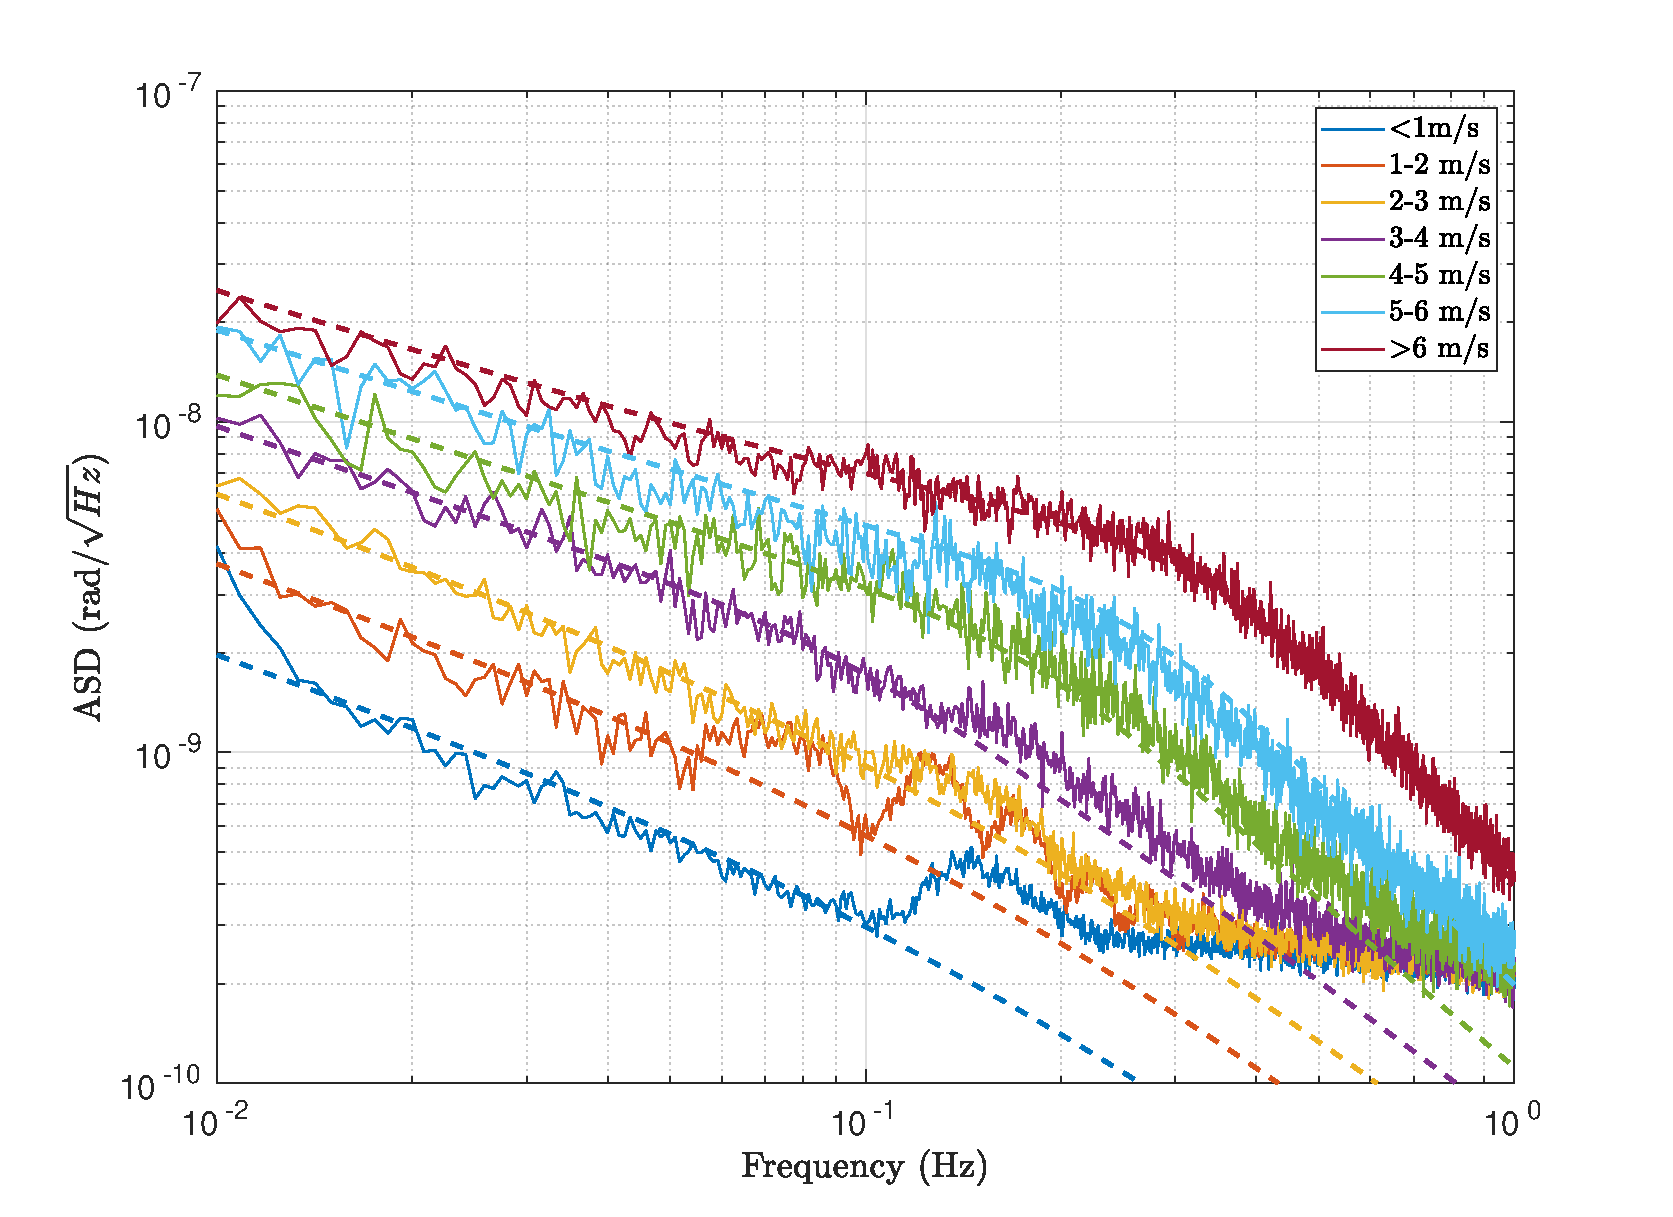
\includegraphics[width=\textwidth]{TiltModel.pdf}
\caption{Observed and modeled tilt vs wind speed for LHO End-X. The solid lines are the measured ground tilt while the dashed are the model. At low wind speeds, the BRS noise and the microseism become dominate at high frequencies.}
\label{tiltModel}
\end{center}
\end{figure}

\subsection{Duty Cycle Improvements}

The figure of merit which most readily displays the improvements in duty cycle due to inclusion of the BRSs is the empirical probability of having the interferometer locked at a given wind speed over the three observing runs. This is shown in Figures \ref{LHO_events} and \ref{LLO_events} for LHO and LLO, respectively. It should be noted that BRSs were implemented at Hanford for both O2 and O3a while Livingston was only for O3a.

\begin{figure}%
\begin{center}
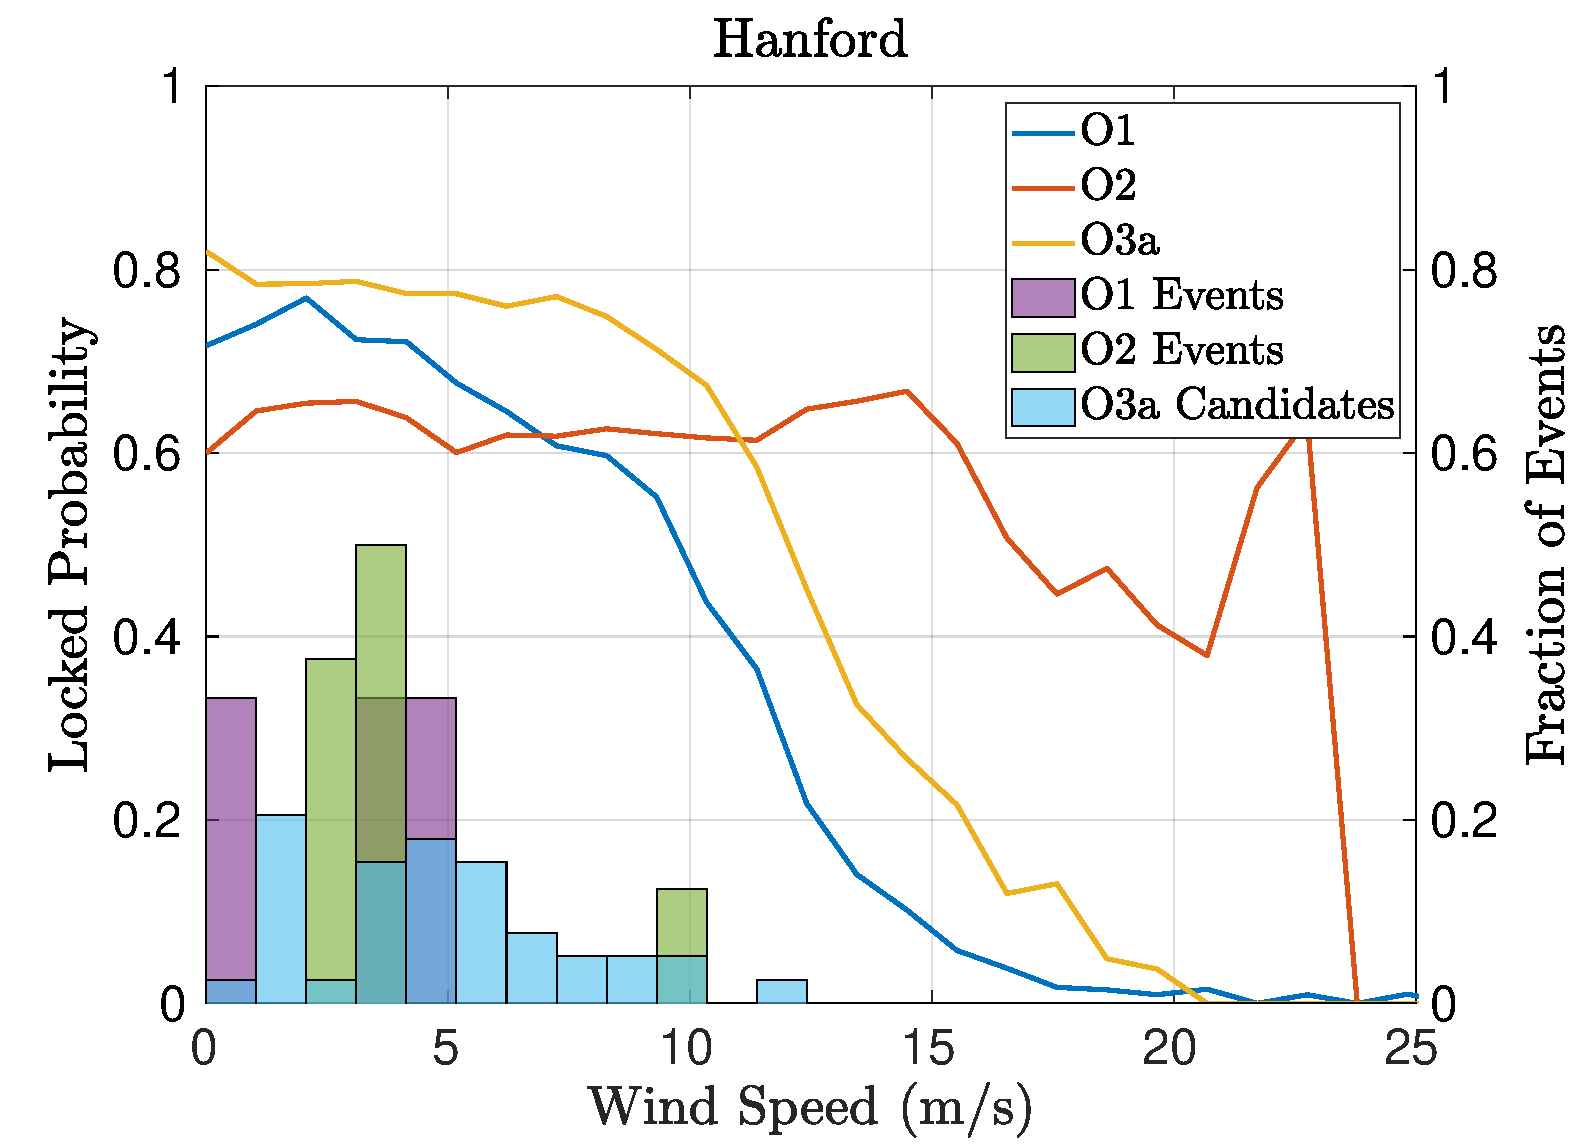
\includegraphics[width=\textwidth]{LHO_WindVsLockEvents.pdf}
\caption{Duty cycle improvements for the LIGO Hanford Observatory. \textbf{Add label on right axis}}
\label{LHO_events}
\end{center}
\end{figure}

For Hanford, the benefit of the tilt subtraction scheme can clearly be seen between O1 and O2 curves. During O1 the locked probability fell monotonically with wind speed, while for O2 the probability stayed relatively constant up to 15 m/s above which it fell steadily. For O3a, Hanford saw a clear decrease in performance at high wind speeds yet still out performed the O1 scheme. This loss of performance is likely due to the \textbf{Y-arm} beam being displaced away from the center of the test masses to avoid point absorbers on the \textbf{Input-Y} test mass. This is known to increase coupling between the angular motion of the test mass and the length measured by the interferometer. This increases the drive needed to keep the interferometer locked and thus increases the susceptibility of the system to increased seismic motion. 

Also shown in Figure \ref{LHO_events} is the fraction of the GW events or candidates detected during O1, O2, and O3a at a given wind speed. This shows that a collection of GW events have been observed whose detection probability is directly increased due to the increase duty cycle at higher wind speeds. Namely, GW170104 was measured at $\sim$\textbf{11} m/s which had an increase in duty cycle of $\sim$\textbf{20 \%} between O1 and O2. Additionally, a number of O3a candidates have been detected above $\sim$\textbf{5 m/s} at which the probability of being locked is increased by $\sim$\textbf{20 \%}.

\begin{figure}%
\begin{center}
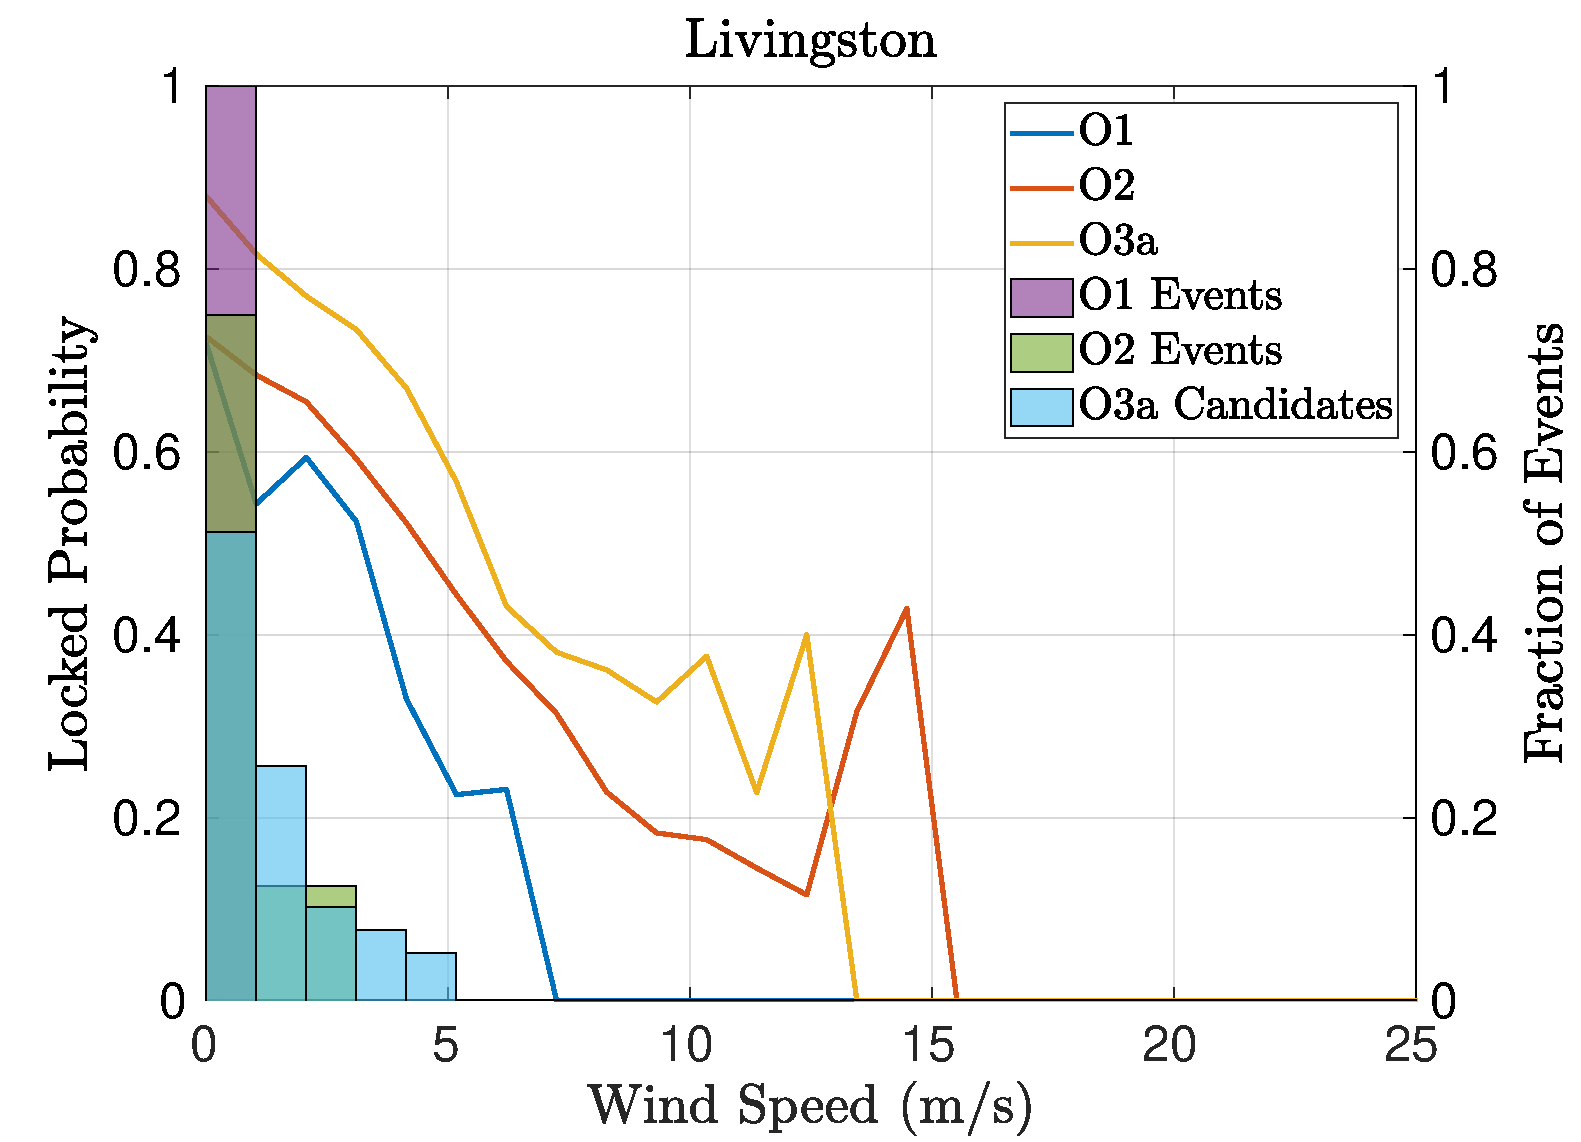
\includegraphics[width=\textwidth]{LLO_WindVsLockEvents.pdf}
\caption{Duty cycle improvements for the LIGO Livingston Observatory. \textbf{Add label on right axis}}
\label{LLO_events}
\end{center}
\end{figure}

At Livingston, the improvements at increased wind speeds is less dramatic as can be seen in Figure \ref{LLO_events}. Although between O1 and O2 tilt subtraction was not implemented, a increase in duty cycle was achieved by implementing a single seismometer for sensor correction on all of the corner station platforms. This decreased the differential mode motion at higher wind speeds and thus made the interferometer lock more robust. An addition increase in performance can be seen between O2 and O3a due to the deployment of tilt subtraction. However, the probability of being locked still dropped monotonically with wind speed, similar to the O1 performance of Hanford.

Despite this, there is a collection of O3a candidates detected between \textbf{3-6 m/s} which are more probable with the increased robustness against wind speed.

\textbf{talk about mean?}
\textbf{maybe plot of mean or expectation vs observing run}

\chapter{30-cm Scale On-Board Rotation Sensors}\label{cBRS_chap}
\section{Angular Controls}
To operate the LIGO interferometers in their optimal configuration, the angular motion of the test masses in the pitch degree of freedom must be under \textbf{number} nrad/$\sqrt{\text{Hz}}$ at \textbf{number} Hz. The ground rotates at $\sim$\textbf{number} nrad/$\sqrt{\text{Hz}}$ at \textbf{number} Hz. To achieve this desired performance, the seismic isolation operated in the rotational degrees of freedom as well as the translation. Additionally, the upper three masses of the quadruple pendulum are actively actuated at frequencies between \textbf{number} and \textbf{number} Hz to decrease any residual motion.

With the current system, at \textbf{number} Hz the seismic isolation is limited by the sensor noise in the seismometer pair which forms the pitch sensor. This then increases the residual motion due to tilt contamination, described in Section \ref{tiltCon}. To eliminate this residual, high gain feedback loops are required on the angular control loop downstream, which themselves are limited by their respective sensor noise at \textbf{number} Hz. This left over noise then leaks into the gravitational wave band between \textbf{number} and \textbf{number} Hz due to the inability to sharply roll off the control without interfering with sensor noise at lower frequencies.

\begin{figure}
\begin{center}
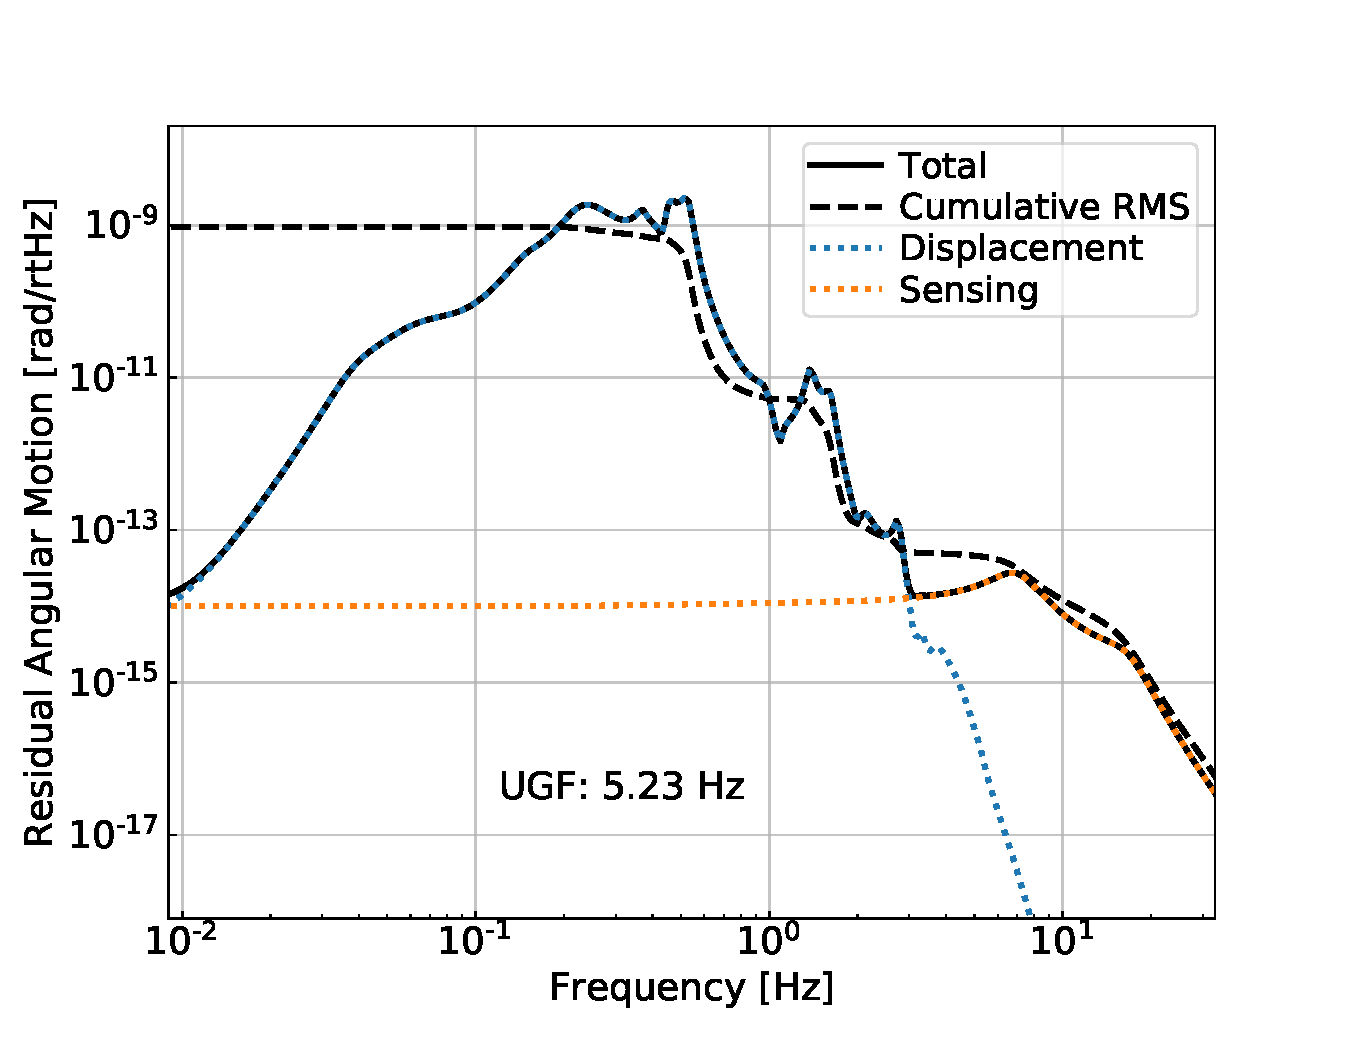
\includegraphics[width=\textwidth]{cBRS_ASC_Without.pdf}
\caption{Performance of the current angular sensing and control system.}
\label{ascWithout}
\end{center}
\end{figure}


The compact Beam Rotation Sensor (cBRS), described in the following, was designed to be an alternative angular sensor for the seismic isolation system with \textbf{number} times lower noise than the current sensors. With this decreased noise, the seismic isolation control loops can be tuned to significantly increase the performance of both the translational isolation, through decreased tilt contamination described in Section \ref{}, and directly the rotational isolation. Details of this follow in Section \ref{IsoScheme}. This decreased residual rotation would then allow the angular control loops to be retuned, specifically decreasing the unity gain frequency, to push the sensor noise leakage closer to the LIGO design sensitivity.

\begin{figure}%
\begin{center}
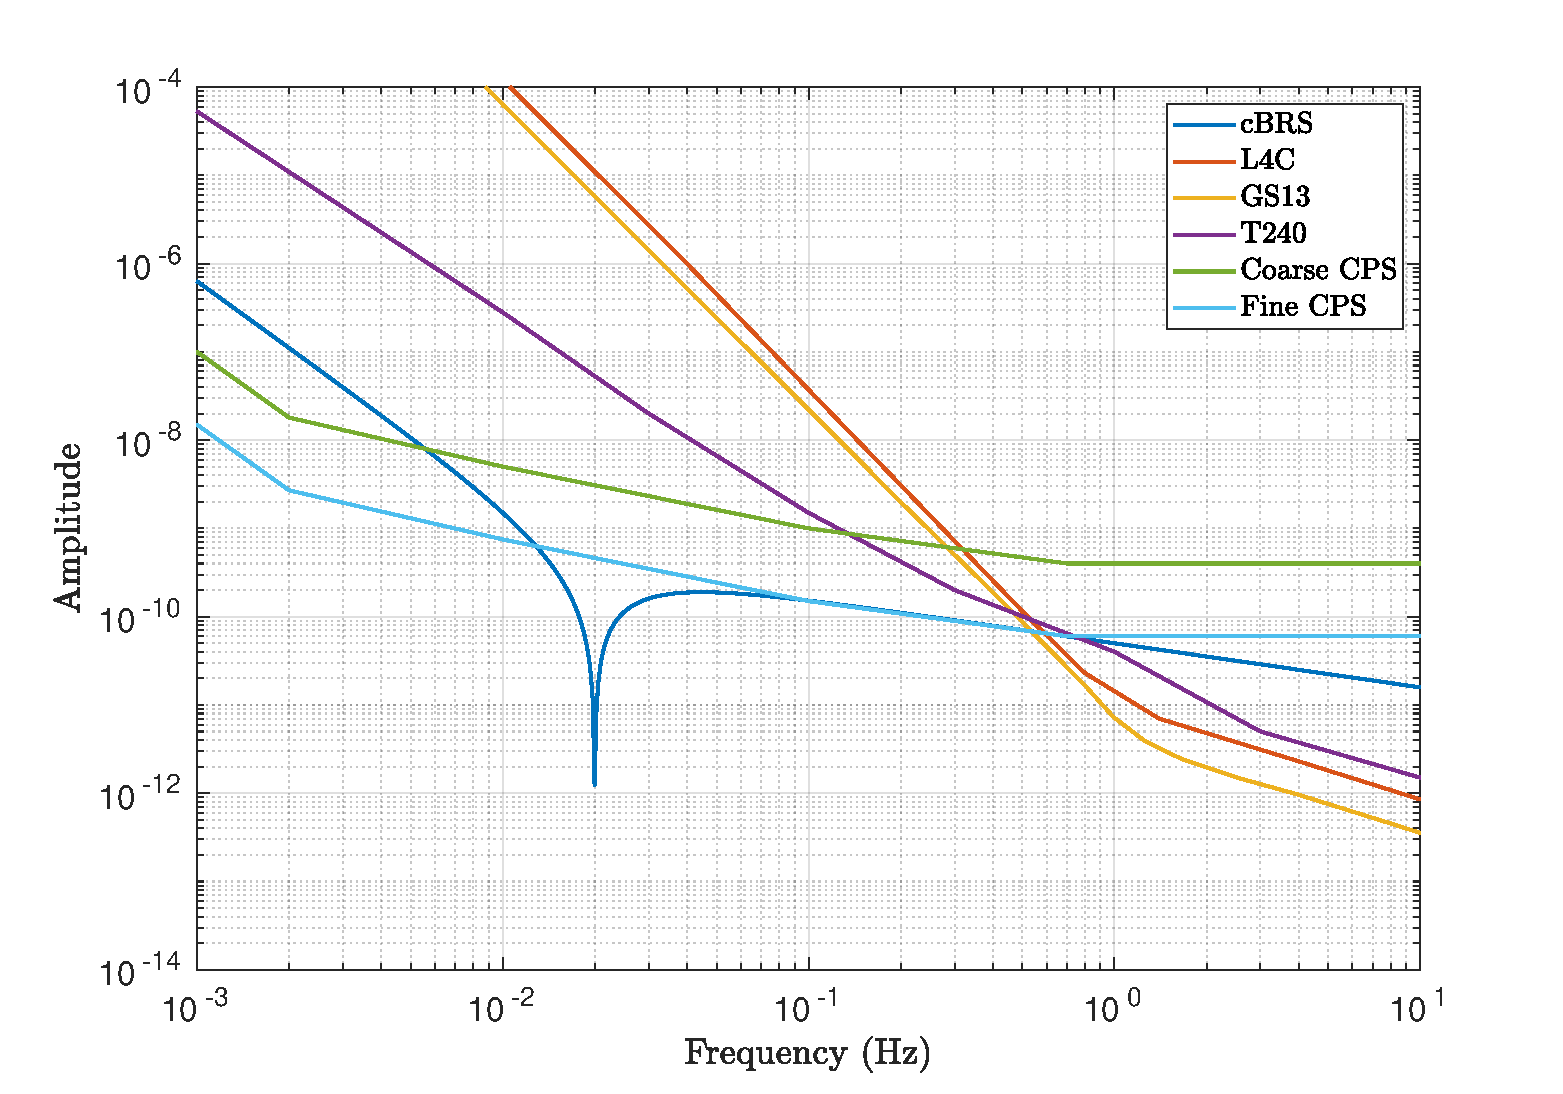
\includegraphics[width=\textwidth]{cBRS_Model_Noise.pdf}
\caption{Theoretical noise curves for the cBRS, blue, and seismometer pair located 1-m apart.}
\label{sensNoise}
\end{center}
\end{figure}


\section{Compact Beam Rotation Sensor} \label{cBRSSec}
\subsection{Mechanical System}

Similar to the BRS described in Chapter \ref{BRS_chap}, the compact Beam Rotation Sensor (cBRS), shown in Figure \ref{cBRS}, consists of a 30-cm long cross hung from 10-15 $\mu$m thick beryllium-copper flexures and has an identical operating principle as the BRS. The cross shape of the balance decreases the sensitivity of the device to gradients in the local gravitational field while allowing for increased moment of inertia compared to a similarly sized beam. 

This design yields a resonant frequency of $\sim$20 mHz which limits the use of such a device with high fidelity to frequencies above this. This removes the possibility of using such a device for ground tilt subtraction since the relevant ground tilts happen below 40 mHz. 

\begin{figure}[!h]
\begin{center}
\includegraphics[width=0.75\textwidth]{cBRSIso.png}
\end{center}
\caption{CAD rendering of the compact BRS (cBRS) showing the cross with its copper end masses which is hung from the flexures from the surrounding support structure. Additionally, the translation stages which hold the fiber interferometer readouts can be seen on either end of the support below the two horizontal end masses.}
\end{figure}


\begin{figure}[!h]
\begin{center}
 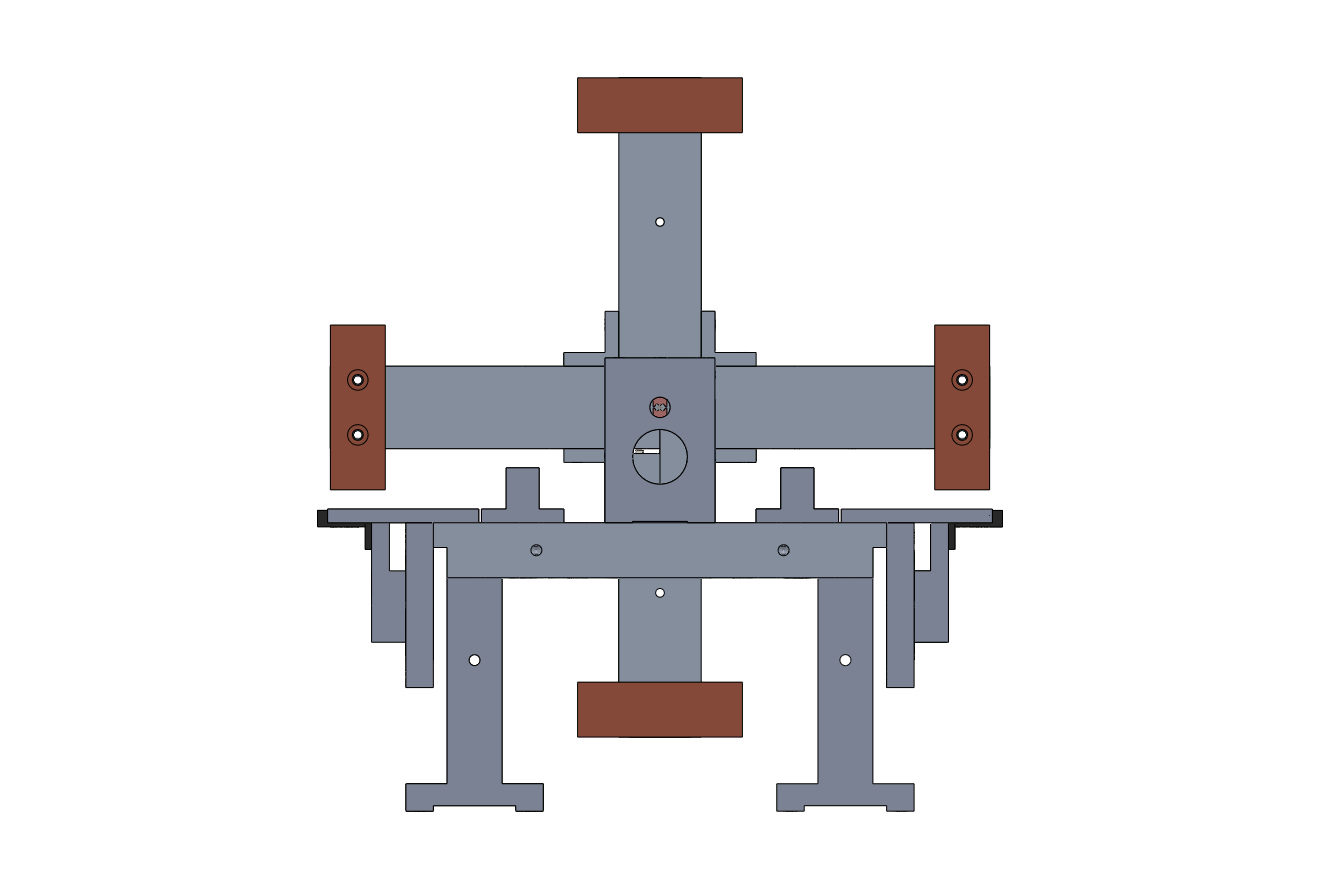
\includegraphics[width=\textwidth]{cBRSFront.png}
 
\caption{CAD rendering of the compact BRS (cBRS) showing the cross with its copper end masses which is hung from the flexures from the surrounding support structure. Additionally, the translation stages which hold the fiber interferometer readouts can be seen on either end of the support below the two horizontal end masses.}
\label{cBRS}
\end{center}
\end{figure}

\subsection{Kinematic Mount}

\begin{figure}[!h]
\begin{center}
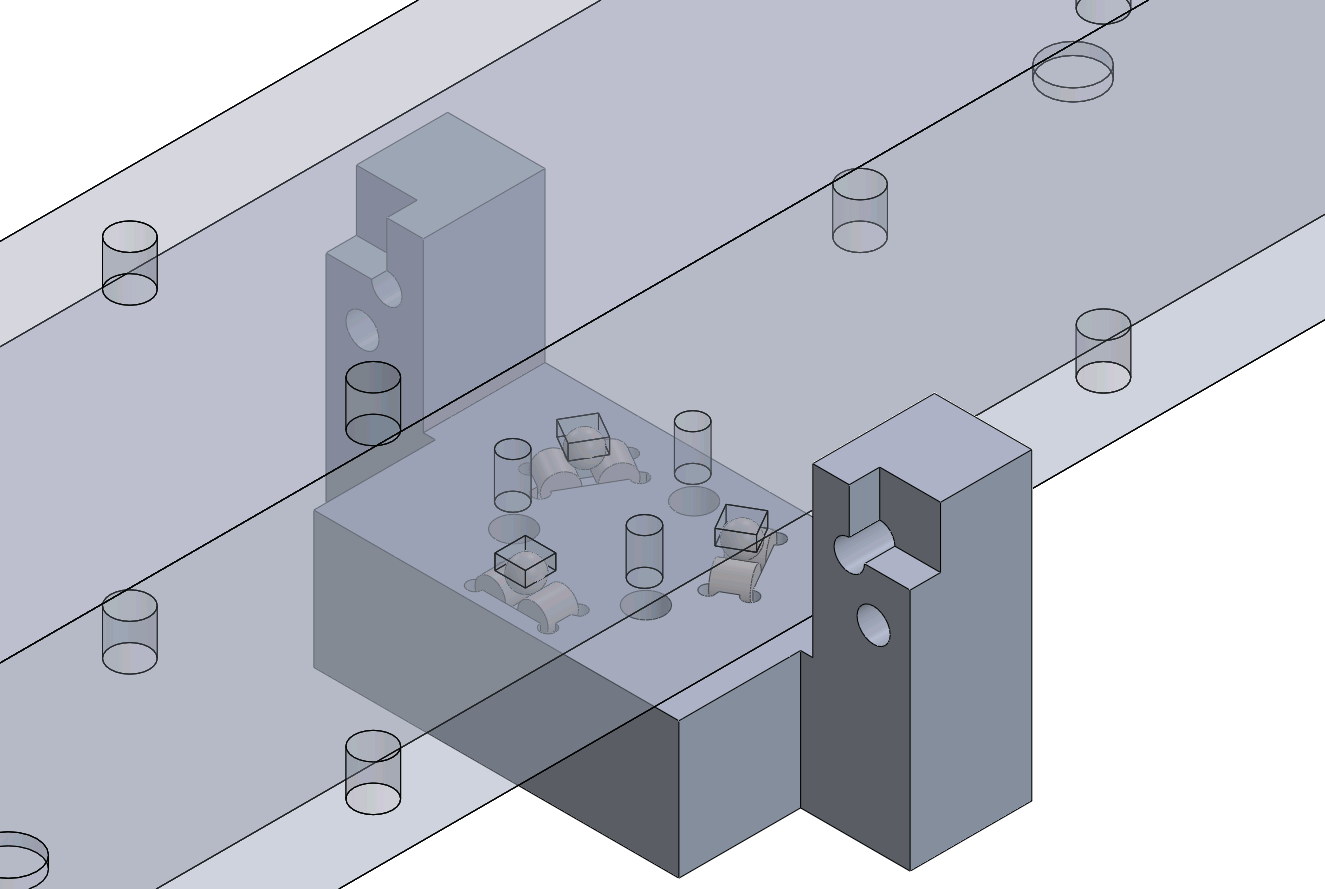
\includegraphics[width=0.75\textwidth]{cBRSKMount.png}
\end{center}
\caption{CAD rendering of the compact BRS (cBRS) showing the cross with its copper end masses which is hung from the flexures from the surrounding support structure. Additionally, the translation stages which hold the fiber interferometer readouts can be seen on either end of the support below the two horizontal end masses.}
\end{figure}

\subsection{Interferometric Readout}
In order to maintain the small size of the entire device and to decrease readout noise, an interferometric readout was developed that consists of a Fabry-Perot cavity that is formed by a beamsplitter coated optical fiber and a full reflecting mirror placed on the bottom of the balance's end masses. The reflectance of this cavity is then monitored by employing a circulator to seperate the incoming and outgoing rays. As the cavity length changes the reflectence undergoes an interference pattern described by:
\begin{align}
R=\frac{1}{1+F \sin(\delta/2 \lambda)}
\end{align}

where $R$ is the reflectance, $F$ is the finesse, $\delta$ is the path length difference, and $\lambda$ is the wavelength.

\begin{figure}[!h]
\begin{center}
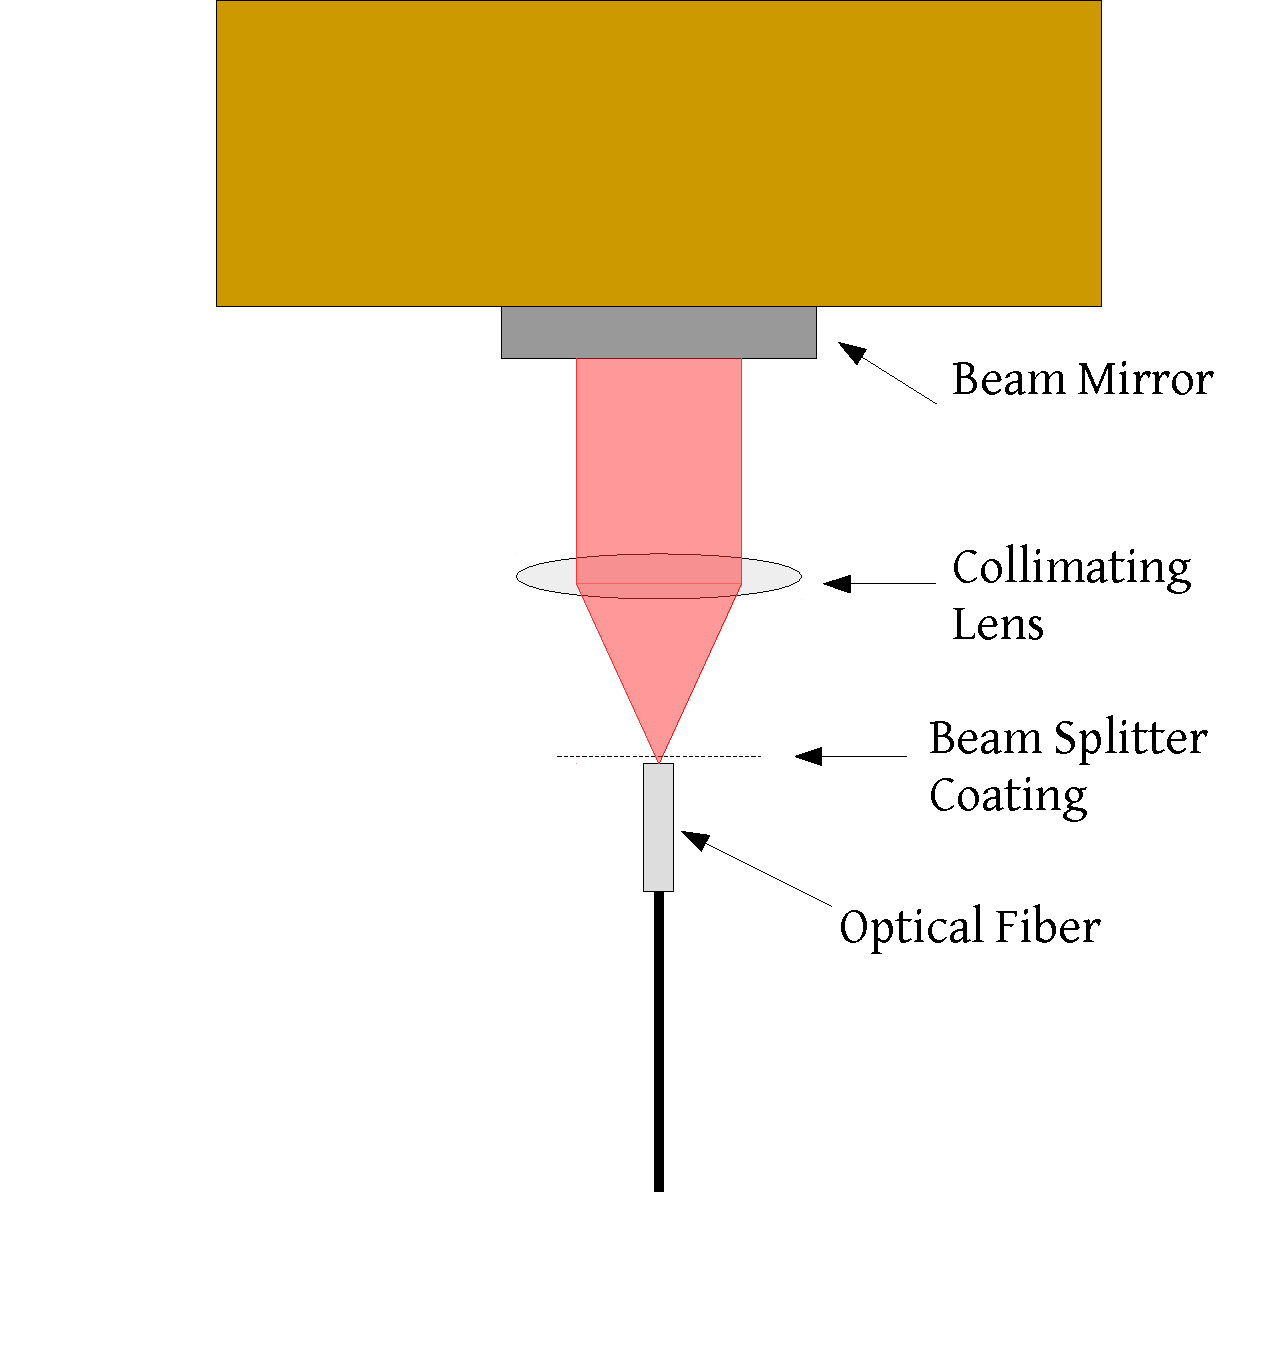
\includegraphics[width=0.5\textwidth]{FiberInt.pdf}
\end{center}
\caption{}
\end{figure}

\begin{figure}[!h]
\begin{center}
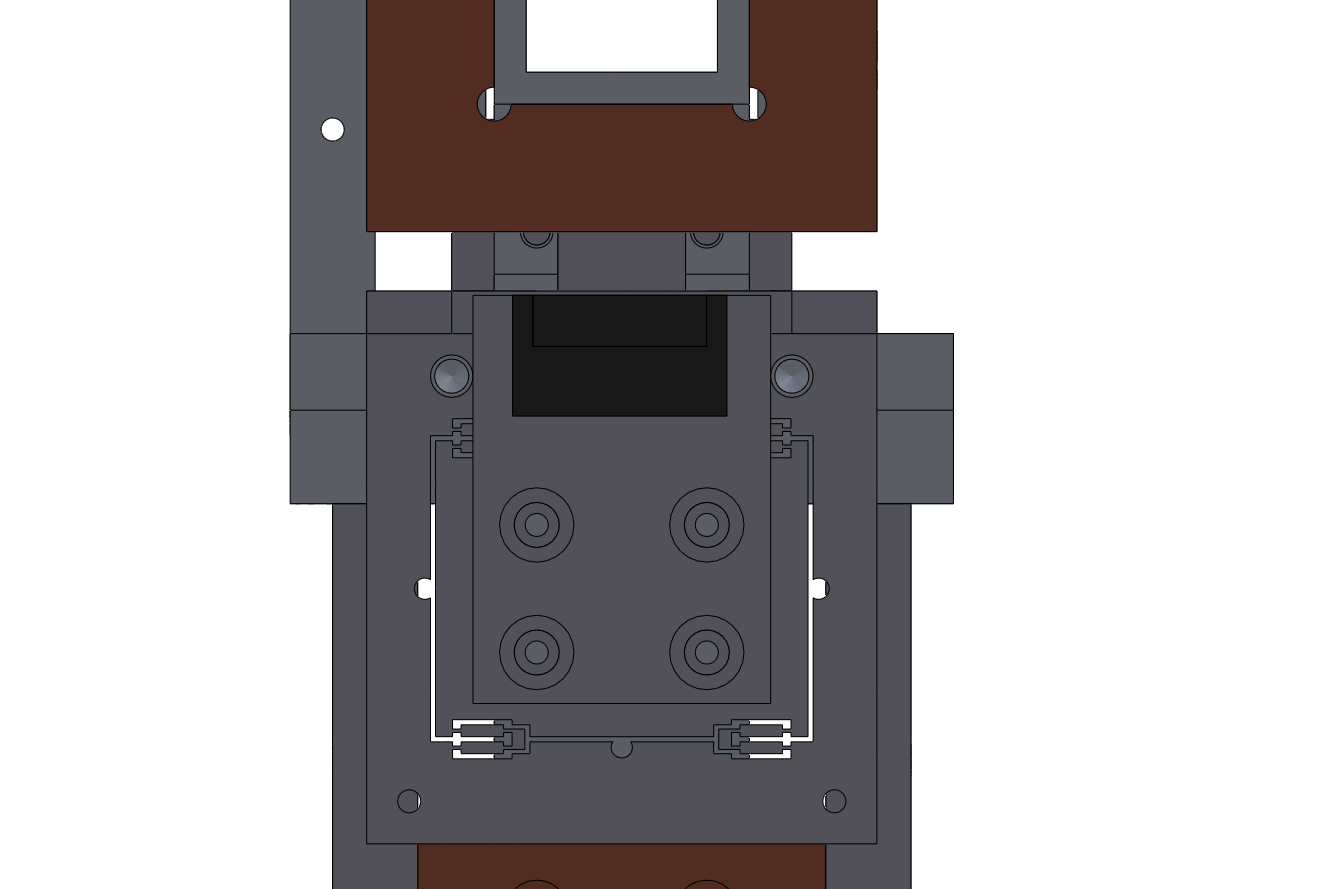
\includegraphics[width=0.75\textwidth]{cBRSOptics.png}
\end{center}
\caption{CAD rendering of the compact BRS (cBRS) showing the cross with its copper end masses which is hung from the flexures from the surrounding support structure. Additionally, the translation stages which hold the fiber interferometer readouts can be seen on either end of the support below the two horizontal end masses.}
\end{figure}

\begin{figure}[!h]
\begin{center}
 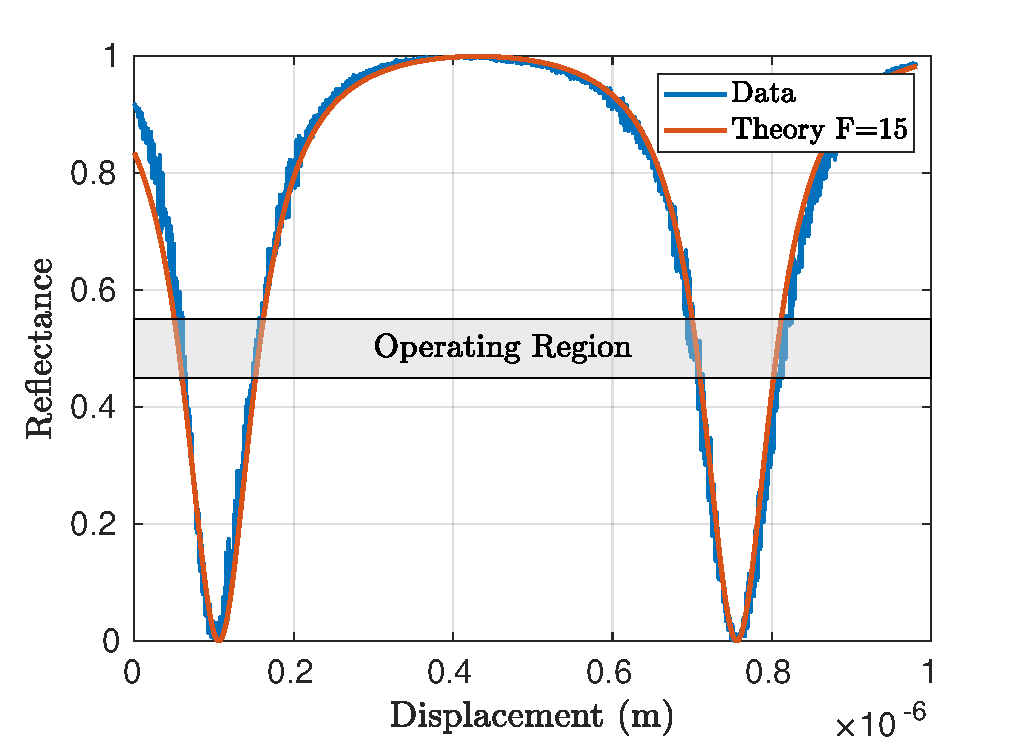
\includegraphics[width=0.75\textwidth]{cBRS_Fringes.pdf}
\caption{Interference pattern of a cBRS fiber interferometer vs cavity length. The gray region is where the device is operated in normal conditions. Within this region the reflectance is approximately linear in displacement.}
\label{cBRS_fringes}
\end{center}
\end{figure}

To linearize this readout, the optical fiber tip and collimating lens are placed on a translation stage that is driven by a piezo stack. The intensity of the reflected light is then fed back to the piezos using a PID loop to hold the cavity length fixed. This allows the system to be seperated into two linear readouts, the interferometer output for small ranges above the unity gain frequency (UGF) of the loop and the control loop output for large motions below the UGF. The output of the device is then the sum of these two channels.

\begin{center}
\begin{tabular}{| c | c |}
\hline
Gain & 0.0005\\
\hline
I & 1000\\
\hline
D & 0\\
\hline
\end{tabular}
\label{pidTable}
\end{center}

\textbf{talk about mccs2}

Although in theory the angle of the beam can be measured with a single interferometer, two readouts are deployed, one at the end of each arm, in order to allow for suppression of common mode noise. The signal seen in each readout is described in Equations \ref{th1} and \ref{th2}. 

\begin{align}
\theta_1&=\theta_s+x_1/L+x_1 \delta_\lambda/\lambda^2+n_c+n_1 \label{th1} \\
\theta_2&=-\theta_s+x_2/L+x_2 \delta_\lambda/\lambda^2 + n_c+n_2 \label{th2}
\end{align}

Where $\theta_{1,2}$ are the angle equivalent signal seen in readout 1 and 2, $\theta_{s}$ is the sensed angle, $x_{1,2}$ are the length of the respective cavities, $L$ is the arm length of the beam, $\delta_\lambda$ is the change in wavelength of the laser, $\lambda$ is the wavelength of the laser, $n_c$ is the sum of all unmodeled common noises, and $n_{1,2}$ are the unmodeled noises that appear in one readout and not the other.

As the angle of the beam appears with opposite phase in the two readout, the difference between the two, Equation \ref{diffEq}, contains the angle while suppressing common noise. Most notable of these common noise sources is frequency noise of the laser. This couples to the angle only through the mismatch in the average cavity lengths which are matched to within \textbf{1 mm}. On the other hand, the sum of the two channels, Equation \ref{sumEq}, contains no contribution from the angle but is instead comprised of only noise sources and thus allows for the in situ measurement of the sum of noises.


\begin{align}
\Delta \theta&=2\theta_s+ (x_1-x_2)\delta_\lambda/\lambda^2+n_1-n_2 \label{diffEq} \\
\Sigma \theta&=(x_1+x_2)/L+ (x_1+x_2)\delta_\lambda/\lambda^2+2n_c+n_1+n_2 \label{sumEq}
\end{align}

\textbf{include plot of loop shape}

\textbf{mention PID tuning}

\subsection{Calibration}

The two readouts are calibrated independently to take into account differing piezo calibration and amplifier gains. The calibration is done by driving the piezo linearly through its entire range while the beam is locked. During this drive the interference pattern wraps through multiple fringes as the cavity length is decreased. The minima of these fringes is known to be separated by $\lambda/2$ which allows for the calibration from voltage across the piezo to displacement. The region around the 50\% reflectance point is then fit to a linear function of displacement to yield a calibration from reflectance to displacement.  

This calibration scheme requires independent determination of the wavelength of the laser which is specified by the manufacturer to be 1310 nm \textbf{$\pm$ 10\%}. Additionally, this assumes that the pattern seen at the photodiode is the interference due to the Fabry-Perot cavity formed by the beam splitter coating and the mirror on the beam. This was verified by comparing the refelctance measurements to the theory as can be seen in Figure \ref{cBRS_fringes}.

\textbf{include calibration numbers}

\begin{figure}%
\begin{center}
 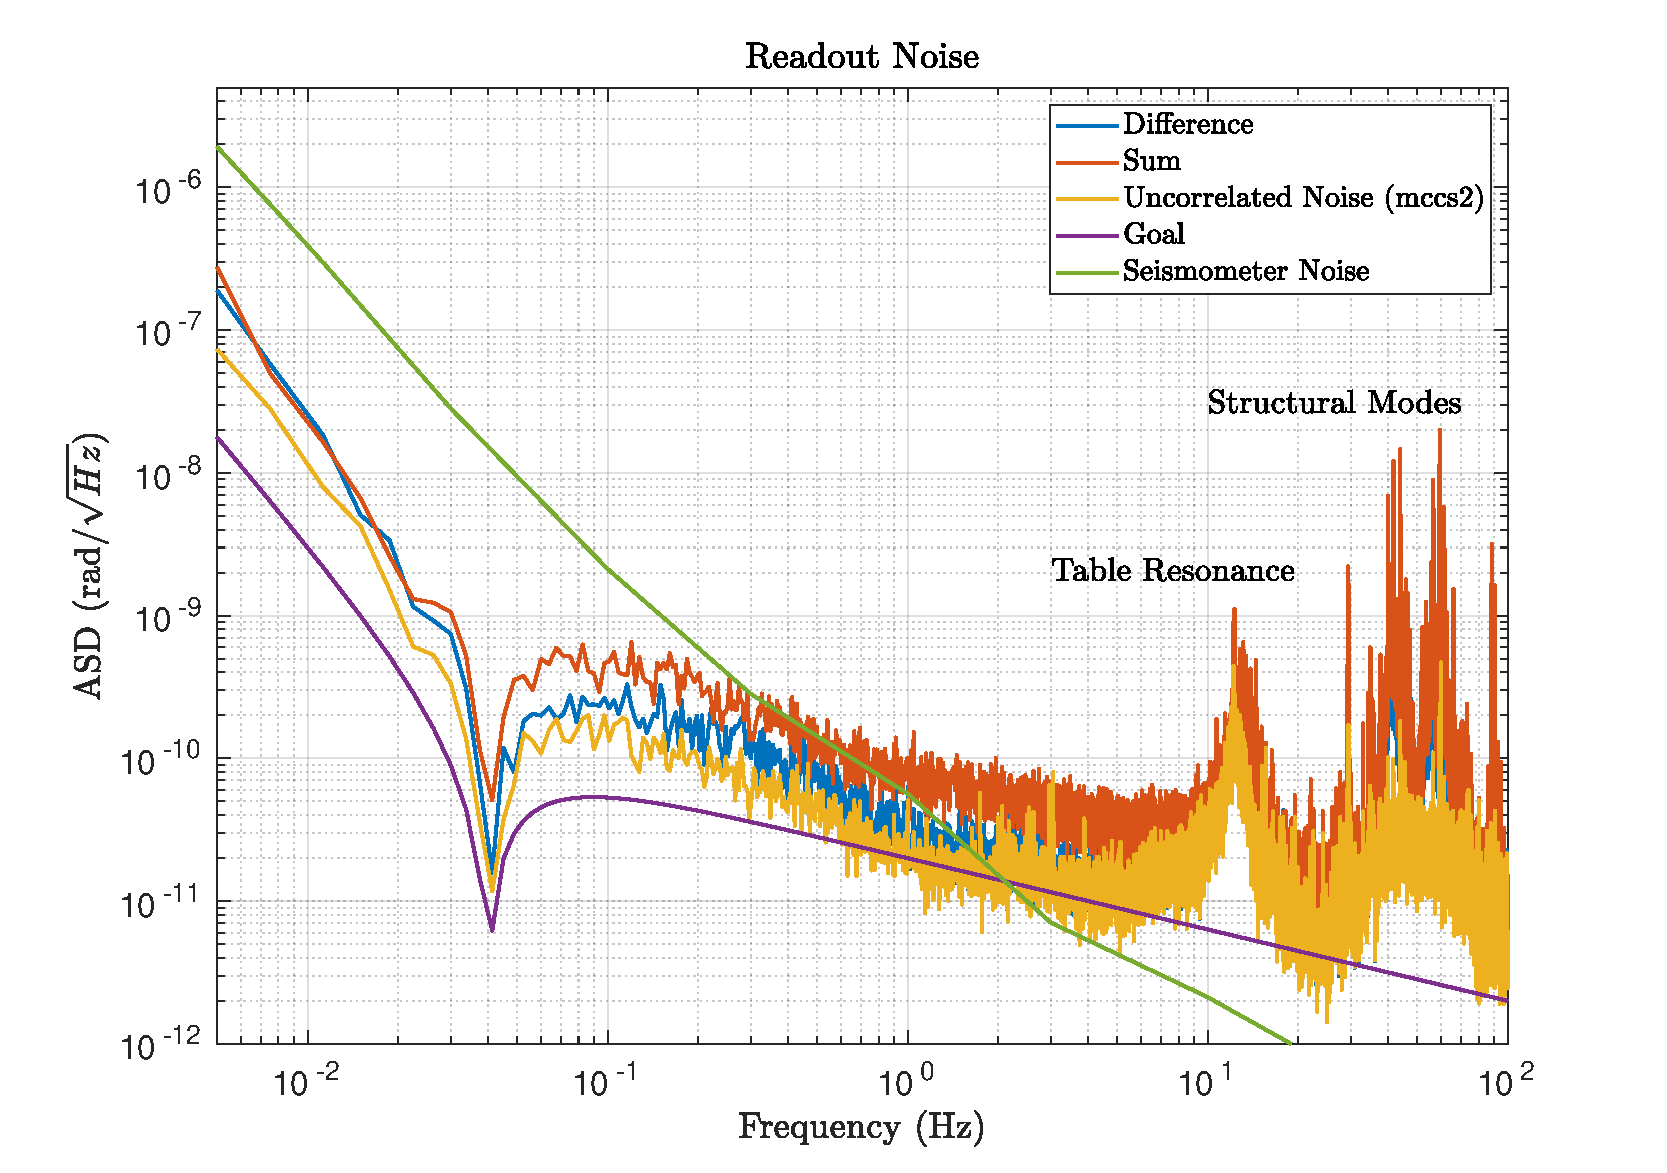
\includegraphics[width=\textwidth]{cBRS_ReadoutNoise.pdf}
\caption{Readout noise of the cBRS with the beam mechanically locked in place. The red is the sum of the two fiber interferometers, the blue is the difference, the yellow is the maximally subtracted signal, and purple is the design sensitivity. Also shown is the performance of a pair of T240 seismometers which are the current sensors used by LIGO.}
\label{cBRS_readout}
\end{center}
\end{figure}

\subsection{Mass Adjustment}

Through a variety of mechanisms, both the BRSs and the cBRS can undergo long term drifts of the equilibrium position that can drive the beam-balance past the dynamic range of the readout. To counteract this, a mass on the balance can be moved or added to shift the center of mass as such:
\begin{align}
\Delta \theta=\frac{g}{\kappa} m r
\end{align}
where $\Delta \theta$ is the change in equilibrium angle, $g$ is the gravitational acceleration, $\kappa$ is the spring constant of the flexure, $m$ is the mass added, and $r$ is the distance from the mass and the pivot point.

While for the BRS the horizontal center of mass (COM) was designed to be tuned by hand, for the cBRS to operate within the LIGO vacuum chambers this must be done remotely and in an automated fashion. To achieve this a mass adjuster shown in Figure \ref{massAdjust} consisting of a small brass mass on a fine pitched screw is placed on the beam-balance. This allows the shifting of the mass with the rotation of the screw. 

\begin{figure}[!h]
\begin{center}
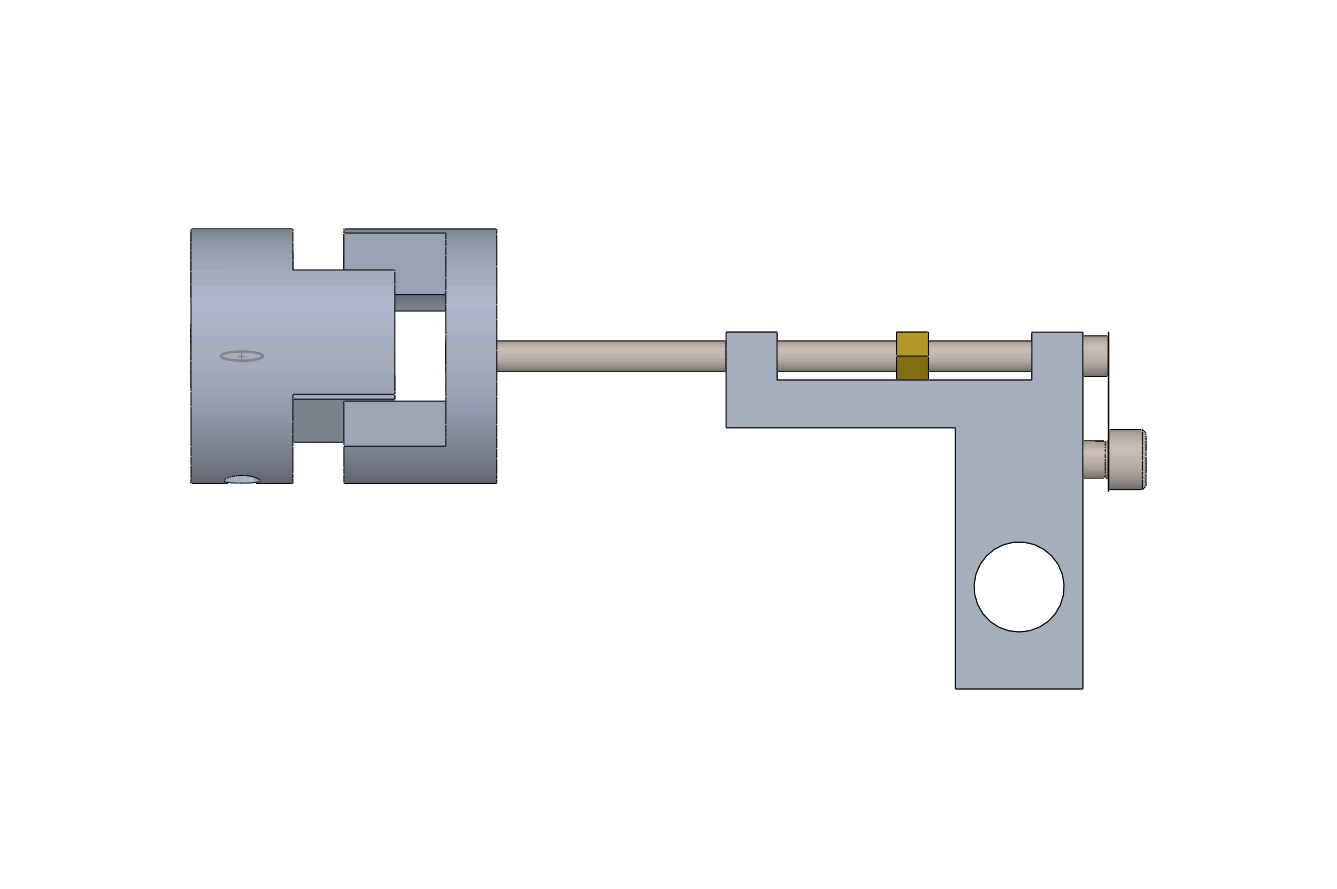
\includegraphics[width=0.75\textwidth]{cBRSMassAdjuster.png}
\end{center}
\caption{CAD rendering of the compact BRS (cBRS) showing the cross with its copper end masses which is hung from the flexures from the surrounding support structure. Additionally, the translation stages which hold the fiber interferometer readouts can be seen on either end of the support below the two horizontal end masses.}\label{massAdjust}
\end{figure}


In order to avoid mechanically shorting the beam balance with wires, the motor which turns this screw is held on an independent support. The couplers between the motor and the screw are intentially oversized to allow for decoupling via back rotations. A small shim of beryllium copper is held tightly against the opposite end of the screw to provide spring loading which hold the screws center of mass in place but allow for rotation.

To test whether this design was capable of moving enough mass accurately, a temporary uncalibrated shadow sensor was set up to measure the motion of the cBRS. The actuation of the mass adjuster can be seen in Figure \ref{massAdjustPlot} which shows the average of period long cuts of the cBRS's resonant motion. In this prototype there is clear hysteresis due to nonuniform friction along the length of the adjuster. However, this was found to not affect the ability to center the cBRS. 

\begin{figure}[!h]
\begin{center}
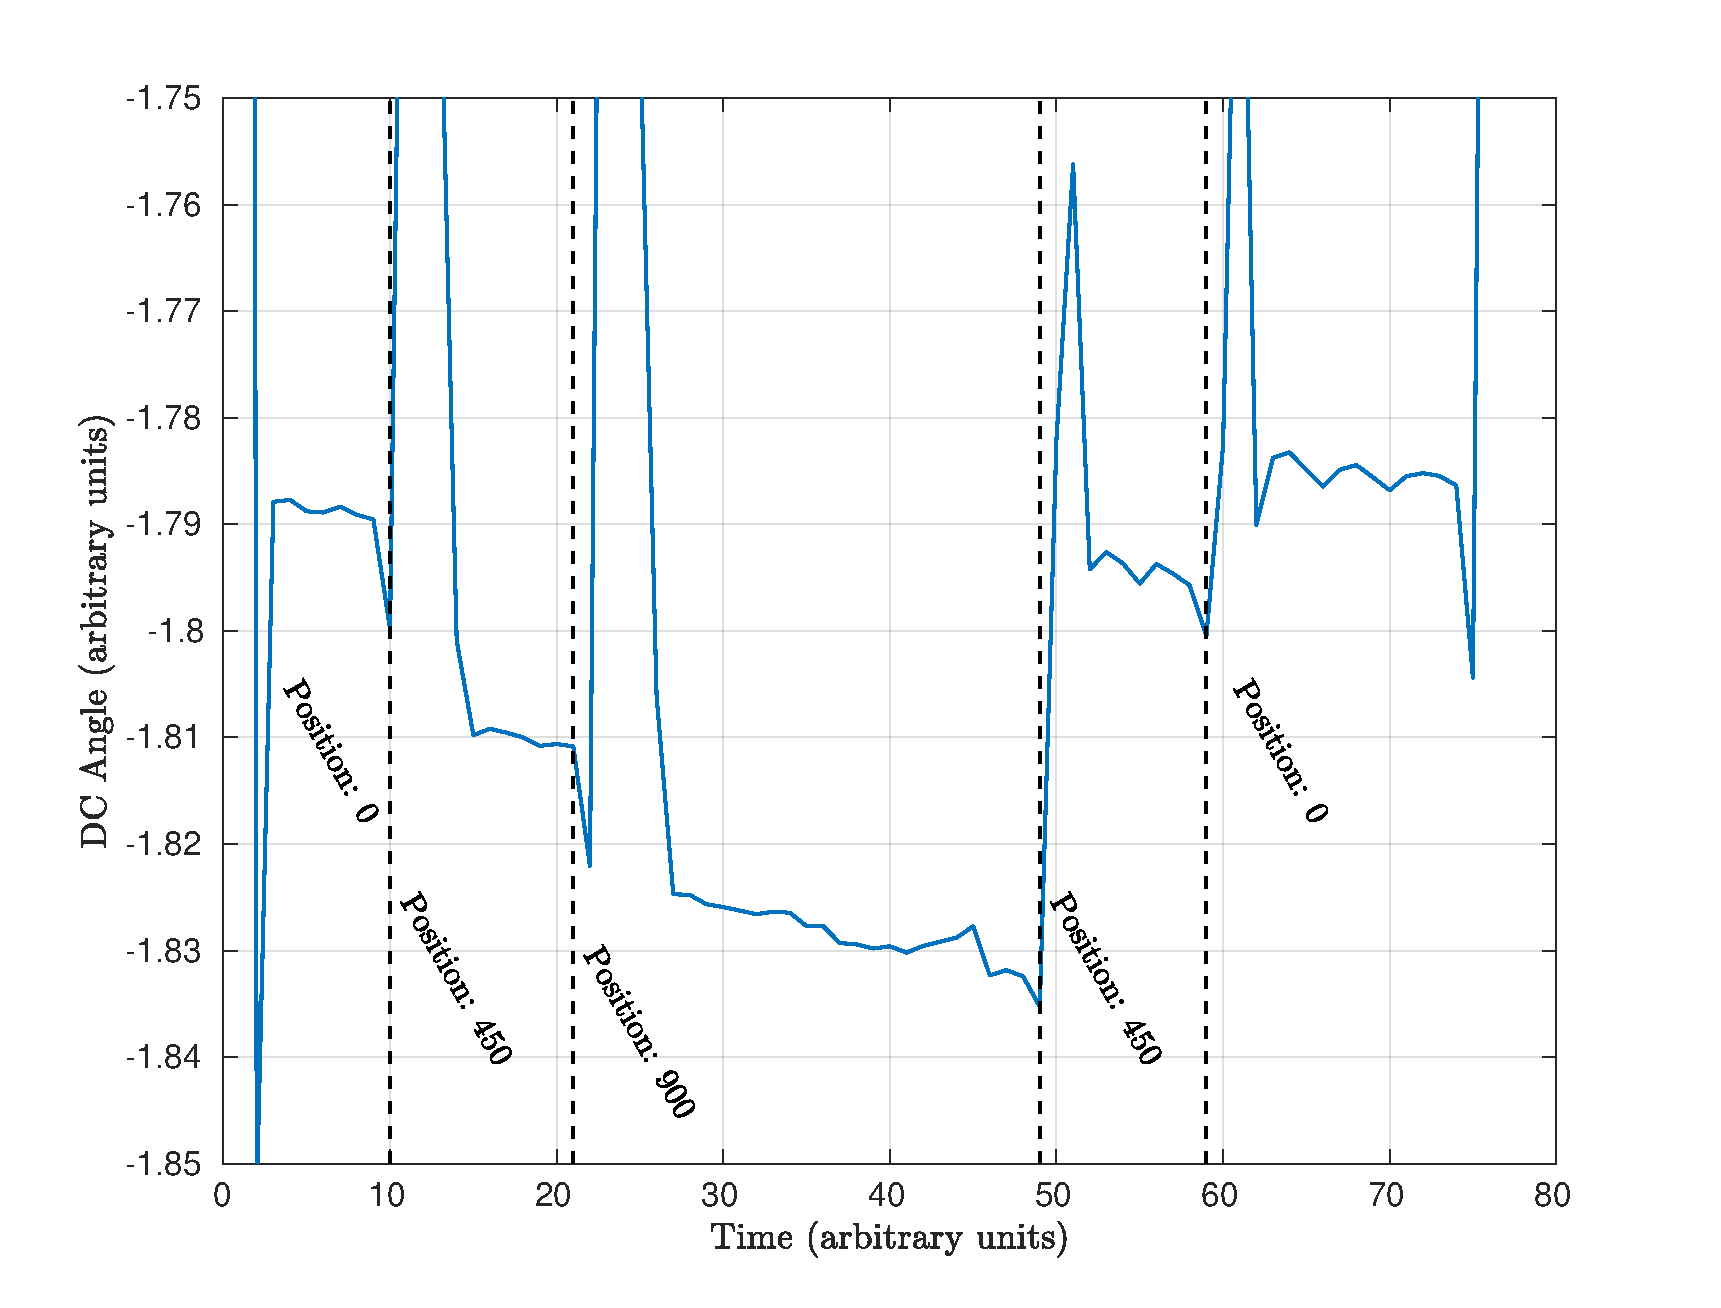
\includegraphics[width=0.75\textwidth]{cBRS_massAdjust.pdf}
\end{center}
\caption{Demonstration of the effect of actuating the remote mass adjuster. The DC angle was measured by taking the mean of period long chunks of shadow sensor data while the mass adjuster was shifted to a collection of positions.}\label{massAdjustPlot}
\end{figure}

\subsection{Controls}

Similar to the BRS controls, the cBRS can be rung up do to environmental transients which can cause resonant motion in excess of the readout's dynamic range. To decrease these amplitudes, two capacitive actuators are placed under the end masses of the beam. These are actuated with low gain with the angular-readout band-passed around the resonant frequency. This allow for low Q motion during high amplitudes and high Q during low amplitudes.

\subsection{Noise Performance}

\begin{figure}
\begin{center}
 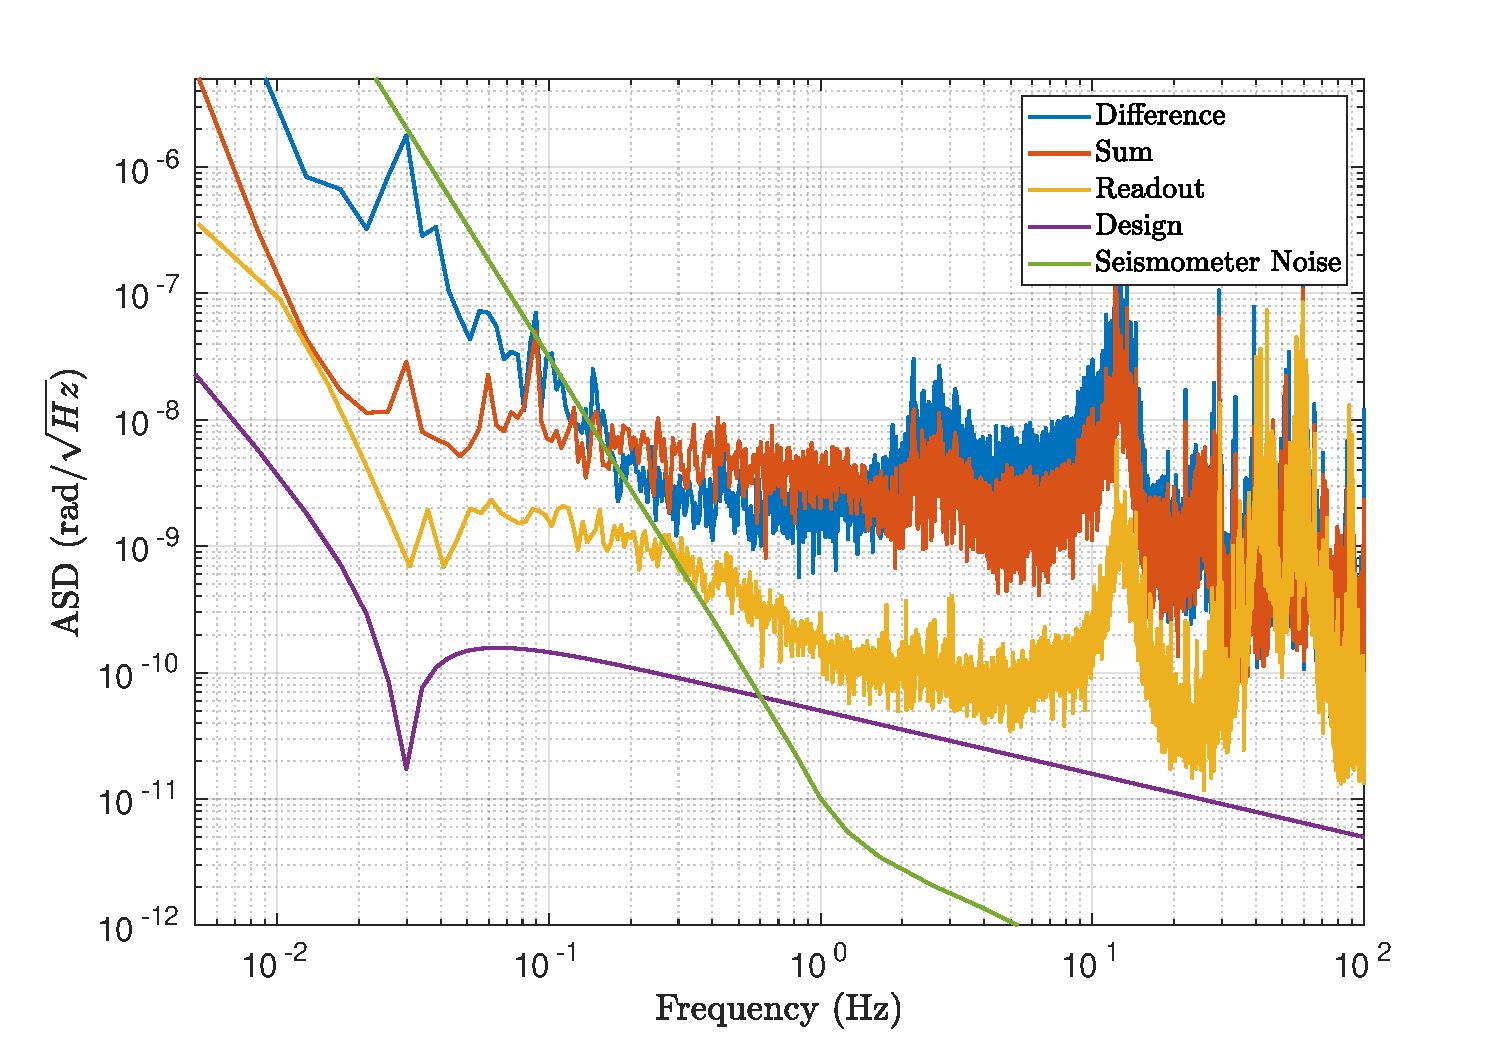
\includegraphics[width=\textwidth]{cBRS_Noise.pdf}
\caption{}
\label{cBRS_noise}
\end{center}
\end{figure}

\textbf{Compare with BRS}

\section{Projected Improvements}
\subsection{Isolation Scheme} \label{IsoScheme}

%Assuming that the isolation is limited by the noise of the in-band sensor, placing the lowest noise sensors on the second stage of the ISI would be expected to yield the lowest angular motion seen by the down stream control loops. With this in mind and the fact that the access to place new sensors is easier for the second stage, a control scheme was modeled which consists of the addition of an idealized cBRS (described in Section \ref{}) on stage 2. This model consisted of only two mechanical degrees of freedom, one horizontal translation and the rotational about the orthogonal horizontal axis.
%
%The rotational control loop for stage 2 then consists of using the CPS between stage 1 and stage 2 at low frequencies, the cBRS at frequencies between 3 mHz and 0.9 Hz, and the GS-13 pairs at frequencies above that. The blend frequencies were tuned to minimized the rms motion at low frequencies while maximizing the isolation at 0.1 Hz. 

As described in Section \ref{seisIso}, each stage and degree of freedom of the seismic isolation system utilizes a blend of multiple sensors as it's feedback signal. These consist of two types of sensors: position sensors which sense motion difference between two stages and inertial sensors which sense the motion relative to an inertial frame. To assess the performance improvements that could be achieved with the addition of a cBRS into the system, a simple two stage, two degree of freedom model was constructed. 

This model assumes both infinite control authority and no dynamics of the isolation platforms. Additionally, purely theoretical models are used for the input motion and the sensor noises. Although a model which accounts for all six degrees of freedom is required to accurately predict the isolation performance, this simplified model is instructive for comparisons of the performance with and without the cBRS.

Throughout this model \textbf{second order binomial filters} are used as the blend filters. In addition, for each stage the inertial sensor noise is taken to be the minimum of the collection of inertial sensors. Realistically these sensors also require detailed blending but the details of this blending is less important below $\sim$ 0.5 Hz. 

\subsubsection{Stage 2 Rotational}

In order to achieve the lowest suspension point motion, we choose to model a cBRS on the second stage of the isolation. This is also the location which currently has enough space to install a device. Due to the rising low frequency noise in the cBRS, tuning where to place the blend frequency becomes a balance of increasing motion at low frequencies and decreasing motion at high and visa versa. The blend frequency was chosen to give a low frequency RMS motion of $\sim$ 10 nrad$/\sqrt{\text{Hz}}$ which matches the performance without the cBRS, see Figure~\ref{cBRSCompR}. This criteria called for a blend frequency of 12 mHz.

The performance with this loop can be seen in Figure \ref{cBRS2R}. Above $\sim$ 500 mHz, the performance is dominated by the GS13 noise and from 80 mHz to 500 mHz it is dominated by cBRS noise. Below 80 mHz, the position sensor contributions become dominate which makes the Stage 2 motion almost equivalent to the Stage 1 motion. The only deviation from Stage 1 motion is near the blend frequency, 12 mHz, where gain peaking added a factor of $\sim$ 3. 

\begin{figure}[!h]
\begin{center}
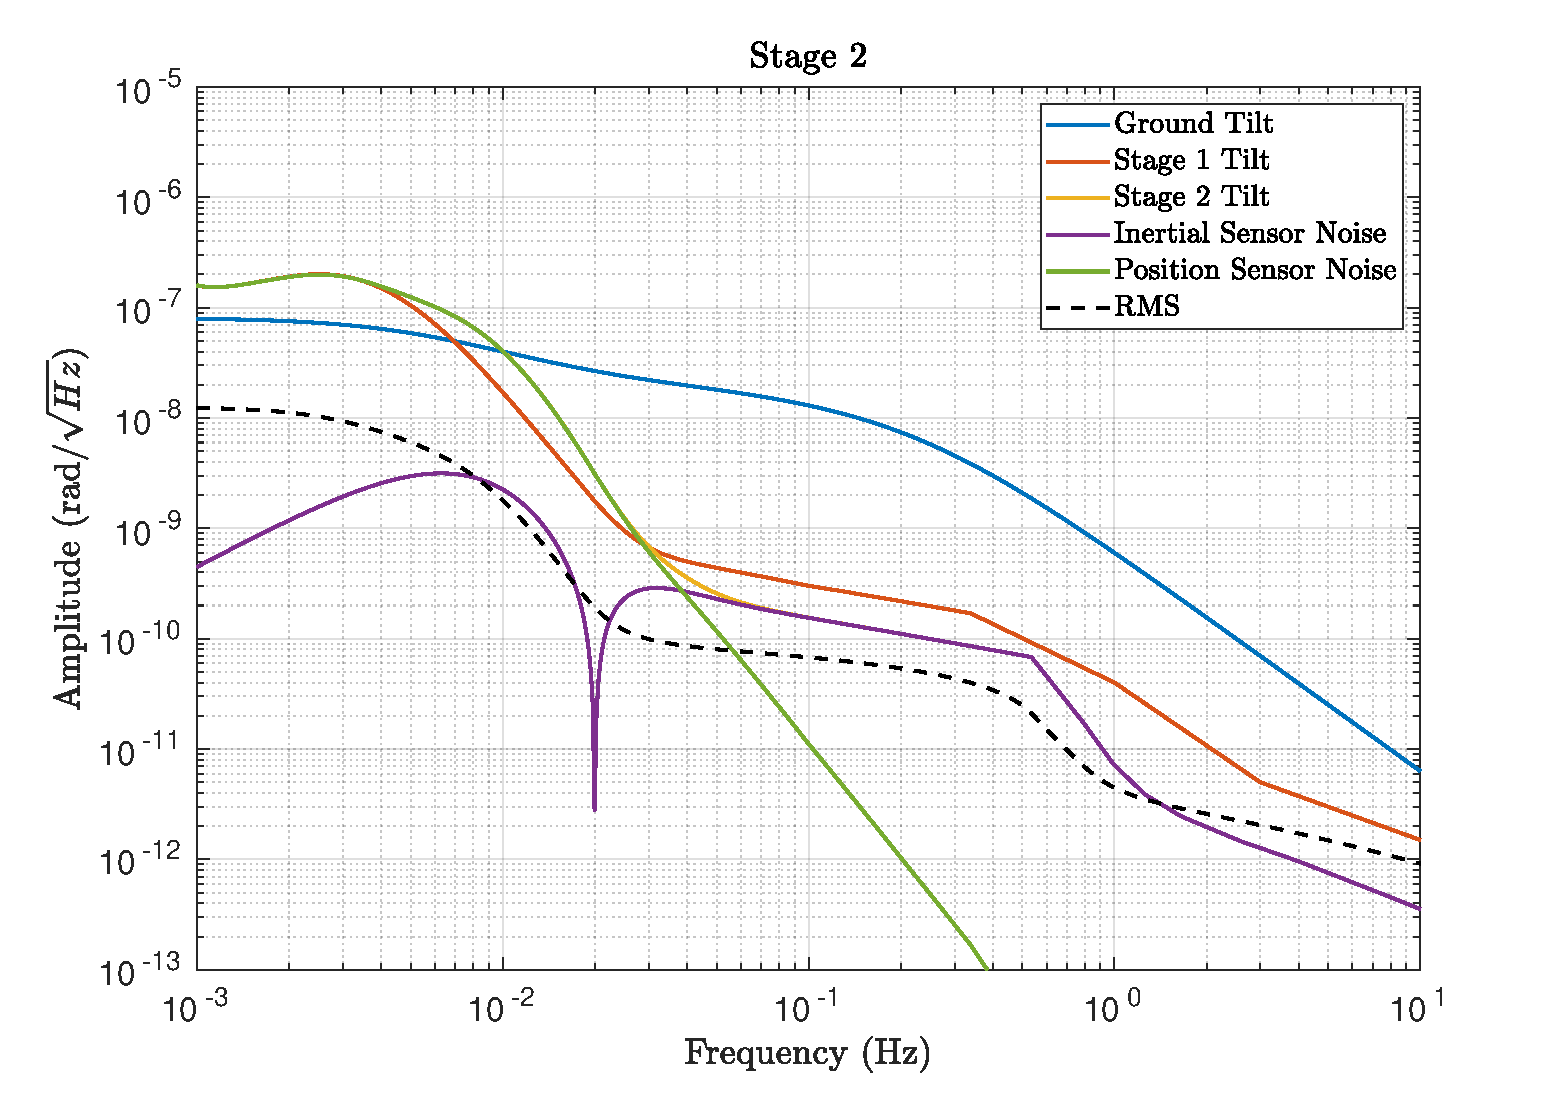
\includegraphics[width=\textwidth]{cBRS_Model_ST2RX.pdf}
\caption{Projected rotational performance of Stage 2 of the ISI with, yellow, and without, red, the cBRS. Also shown is the input ground tilt model, blue, which represents the observed tilt during windy times.}
\label{cBRS2R}
\end{center}
\end{figure}

\subsubsection{Stage 1 Rotational}

With Stage 2 inertially isolated in the rotation degree of freedom above $\sim$ 80 mHz, Stage 1 can achieve superior performance if its control is a combination of the position sensor between the Stage 1 and Stage 2, fine CPS, at high frequencies, and the position sensor between Stage 1 and Stage 0, course CPS, as low. This is effectively using the Stage 2 platform as an inertial proof mass with the fine CPS as a readout. The previous scheme was to use a seismometer pair as an inertial rotation sensor for high frequencies and the course CPS at low. 

\begin{figure}[!h]
\begin{center}
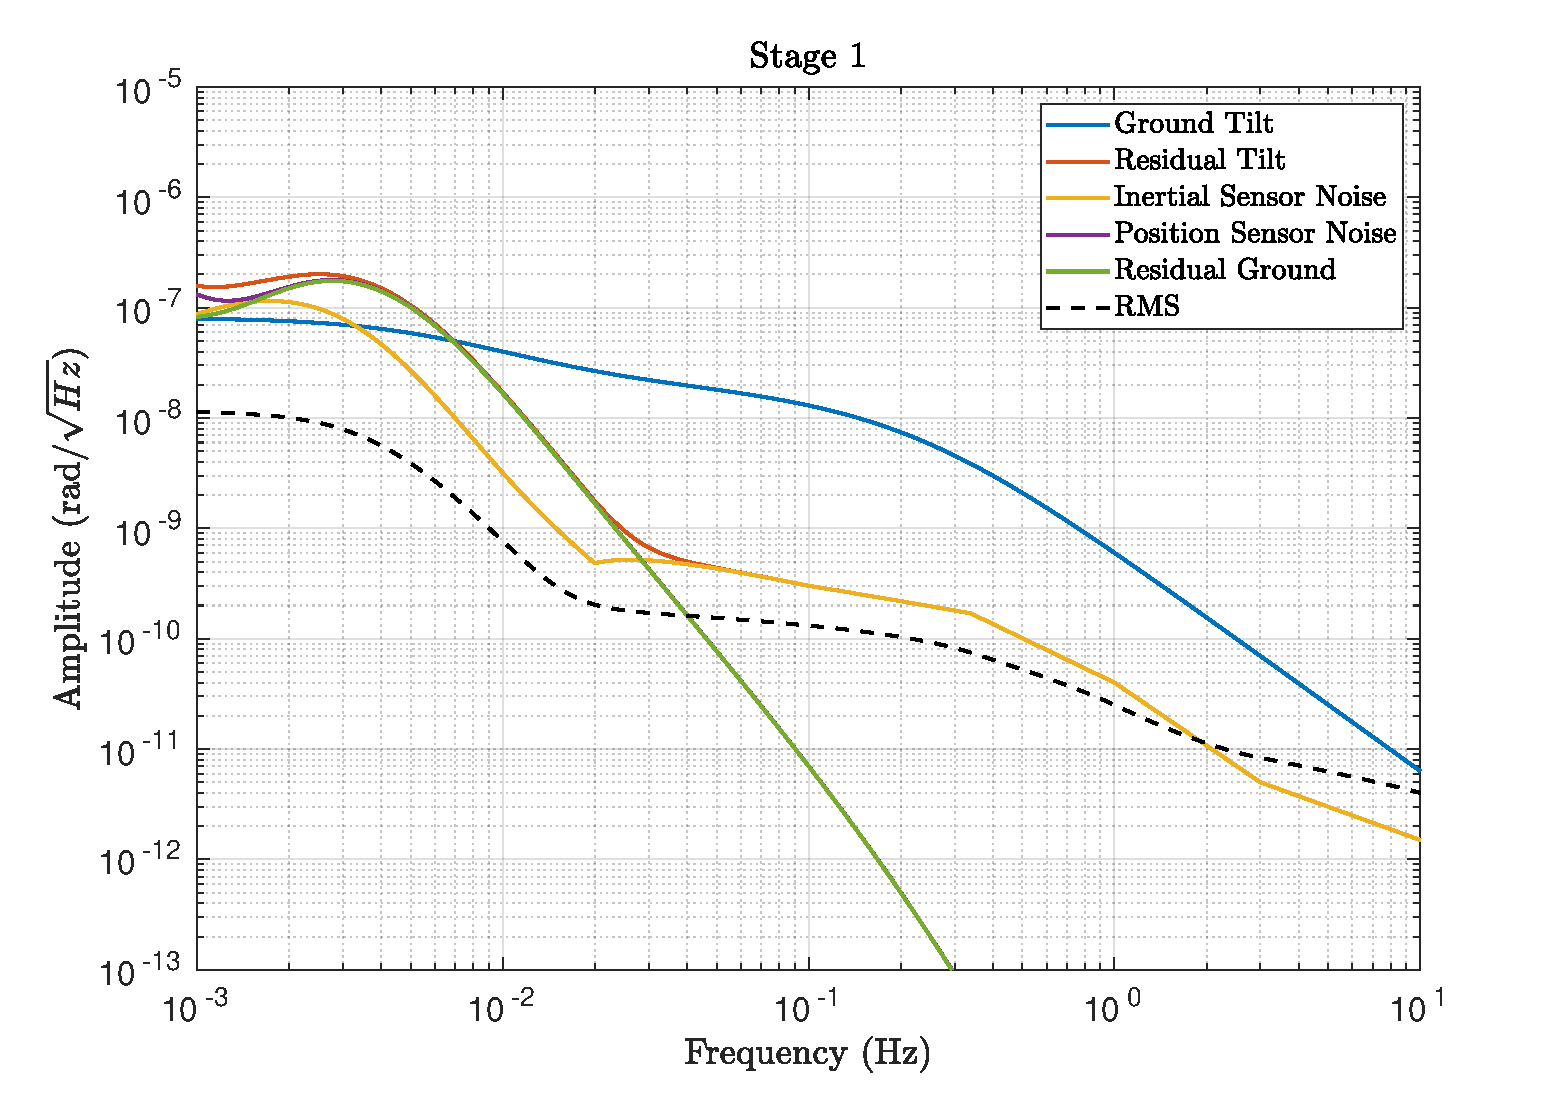
\includegraphics[width=\textwidth]{cBRS_Model_ST1RX.pdf}
\caption{Projected rotational performance of Stage 1 of the ISI with, yellow, and without, red, the cBRS. Also shown is the input ground tilt model, blue, which represents the observed tilt during windy times.}
\label{cBRS1R}
\end{center}
\end{figure}

Applying the same criteria as Stage 2 of requiring low frequency RMS motion of $\sim$ 10 nrad$/\sqrt{\text{Hz}}$ yields a blend frequency of 3 mHz around which the motion is amplified by a factor of $\sim$ 3 because of gain peaking. The performance of this design can be seen in Figure~\ref{cBRS1R} Below 1 mHz, it is expected the platform motion follows the ground but both the ground rotation and sensor noise are not well constrained at low frequency. Above $\sim$30 mHz, the residual is dominated by the combination of the sensor noises from the fine CPS, from 30 mHz to 350 mHz, and the T240 pair, above 350 mHz.

A subtly that arises from using both the fine and course CPS as the control for Stage 1 is that if the Stage 2 blend frequency is placed below the Stage 1 frequency then in between these two frequencies both stages are using the fine CPS as their control. Since the fine CPS measures the motion between the two stages, this effectively makes both stages uncontrolled as they are not referenced to any independent frame. In our model this is avoided by placing the Stage 1 blend frequency a decade lower than the Stage 2 blend.

\subsubsection{Stage 1 Translational}

Once the rotational degrees of freedom are controlled, the translational loops can begin to be tuned. The primary dependence of the traslational performance on the rotational performance comes from tilt contamination of seismometers, described in Section \ref{tiltCon}. As with the rotational control loop design, the choice of blend frequency is a trade off between increasing low frequency motion and decreasing high. We choose to require low frequency RMS performance of $<$ 100 nm/s$/\sqrt{\text{Hz}}$. This requirement is more stringent than the current performance of the seismic isolation \textbf{CHECK}. A blend frequency of 15 mHz was found to exceed this requirement.

The performance of with this choice can be seen in Figure \ref{cBRS1X}. Above 500 mHz, the performance is limited by the T240 noise. Between 25-500 mHz, residual ground motion dominates and between 1-25 mHz residual tilt coupled through tilt contamination of the seismometers is the primary contribution. 

\begin{figure}[!h]
\begin{center}
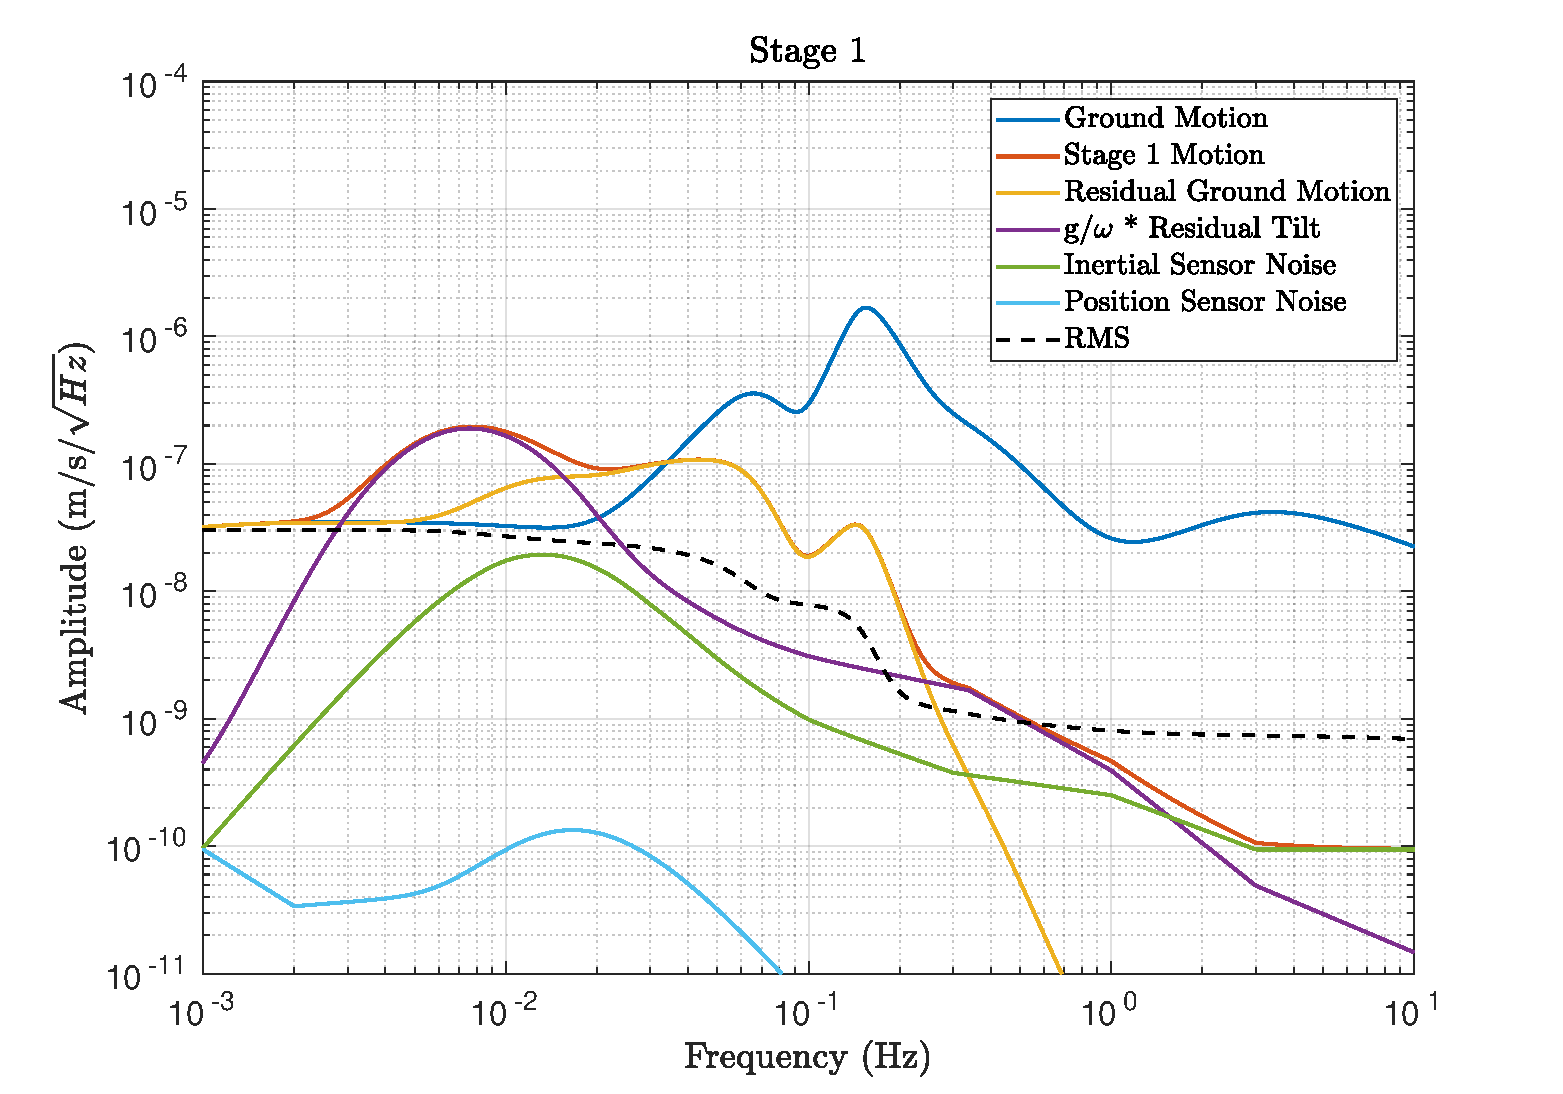
\includegraphics[width=\textwidth]{cBRS_Model_ST1X.pdf}
\caption{Projected translational performance of Stage 1 of the ISI with, yellow, and without, red, the cBRS. Also shown is the input ground motion model, blue, which represents the observed tilt during windy times. The control loops here can be tuned to decrease motion at $\sim$ 100 mHz, the microseism frequencies, by increasing motion at $\sim$ 10 mHz and vice versa.}
\label{cBRS1X}
\end{center}
\end{figure}

\subsubsection{Stage 2 Translational}

The Stage 2 translational loops were tuned in a similar manner as Stage 1: requiring that the RMS motion at 1 mHz be $<$ 100 nm/s$/\sqrt{\text{Hz}}$. This yielded  a blend frequency of 45 mHz. As can be seen in Figure \ref{cBRS2X}, this effectively flattens the residual spectrum between $\sim$ 5-60 mHz to an amplitude of 2-3 $\times 10^{-7}$ m/s$/\sqrt{\text{Hz}}$ while decreasing the microseism at 150 mHz by a factor of $\sim$ 100.

\begin{figure}[!h]
\begin{center}
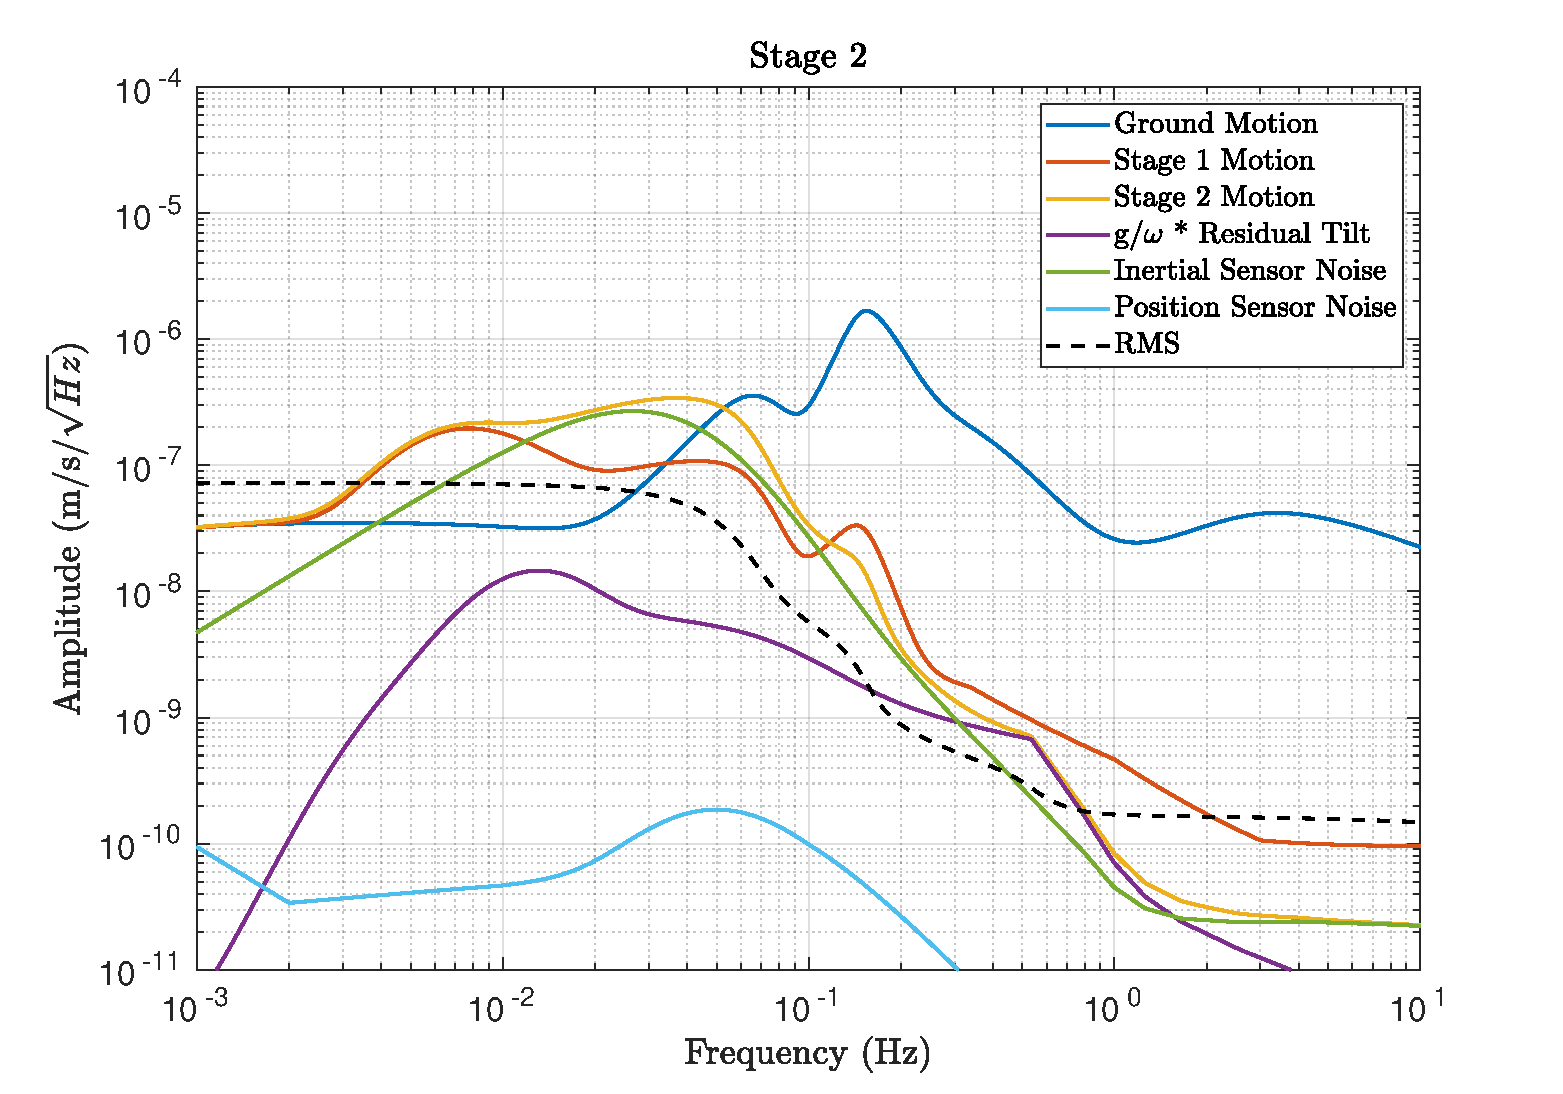
\includegraphics[width=\textwidth]{cBRS_Model_ST2X.pdf}
\caption{Projected translational performance of Stage 2 of the ISI with, yellow, and without, red, the cBRS. Also shown is the input ground motion model, blue, which represents the observed tilt during windy times. The control loops here can be tuned to decrease motion at $\sim$ 100 mHz, the microseism frequencies, by increasing motion at $\sim$ 10 mHz and vice versa.}
\label{cBRS2X}
\end{center}
\end{figure}

Of particular interest for future upgrades to the seismic isolation, the limiting term of the Stage 2 translational performance in these models is the noise due to the on-platform inertial sensors whereas previous performance was dominated by the tilt contamination term. This points to the need of lower noise inertial sensors for future systems. This is an active area of research with many promising candidate sensors \cite{}. 

\subsubsection{Comparison with past performance}

To show the improvements relative to the past isolation system, the performance of the past isolation system was modeled using the same techniques as described in Section \ref{IsoScheme}. The filters used here were those that were in deployment for O2. These are expertly tuned to account for the true performance of the instruments and thus have more complex shapes than the binomial filters used in the proposed isolation scheme.

A comparison of the rotational degree of Stage 2 is shown in Figure \ref{cBRSCompR}

\begin{figure}[!h]
\begin{center}
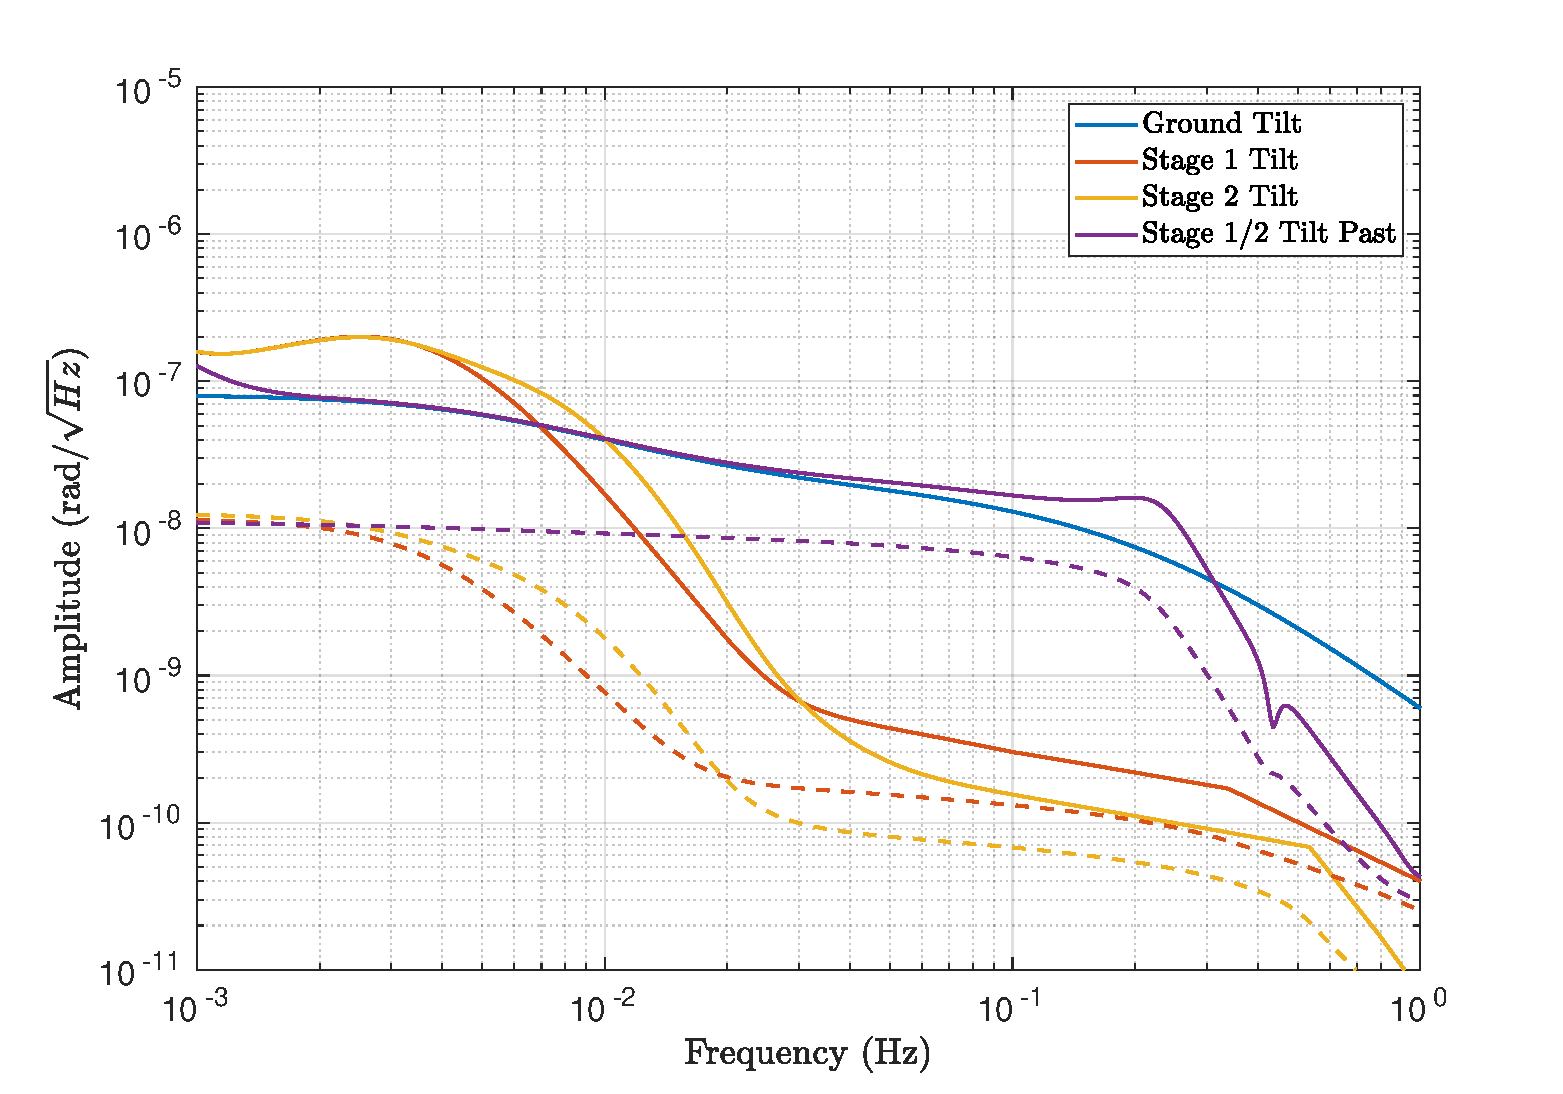
\includegraphics[width=\textwidth]{cBRS_Model_CompRX.pdf}
\caption{Comparison of the rotational isolation performance of Stage 2 during O2 and the projected performance with the inclusion of the cBRS.}
\label{cBRSCompR}
\end{center}
\end{figure}

The performance comparison of the translational degree isolation system is shown in Figure \ref{cBRSCompX}. Above 1 Hz, the performance of the two schemes are similar as lowest noise sensors at those frequencies have not changed. At the secondary microseism, 100-500 mHz, the inclusion of the cBRS yields a factor of $\sim$ 20 improvement of the residual motion while at the primary microseism, 50-100 mHz, it yields a factor of $\sim$ 3. With the cBRS, the residual motion between 3-30 mHz is increased by a factor of ten. However, the RMS motion at those frequencies is still below the previous performance. It is expected that the control loops on the intermediate masses will be able to compensate for this increase in motion without any decrease in performance. Below 2 mHz, both schemes follow the ground since the dominate sensors at those frequencies are the position sensors.

\begin{figure}[!h]
\begin{center}
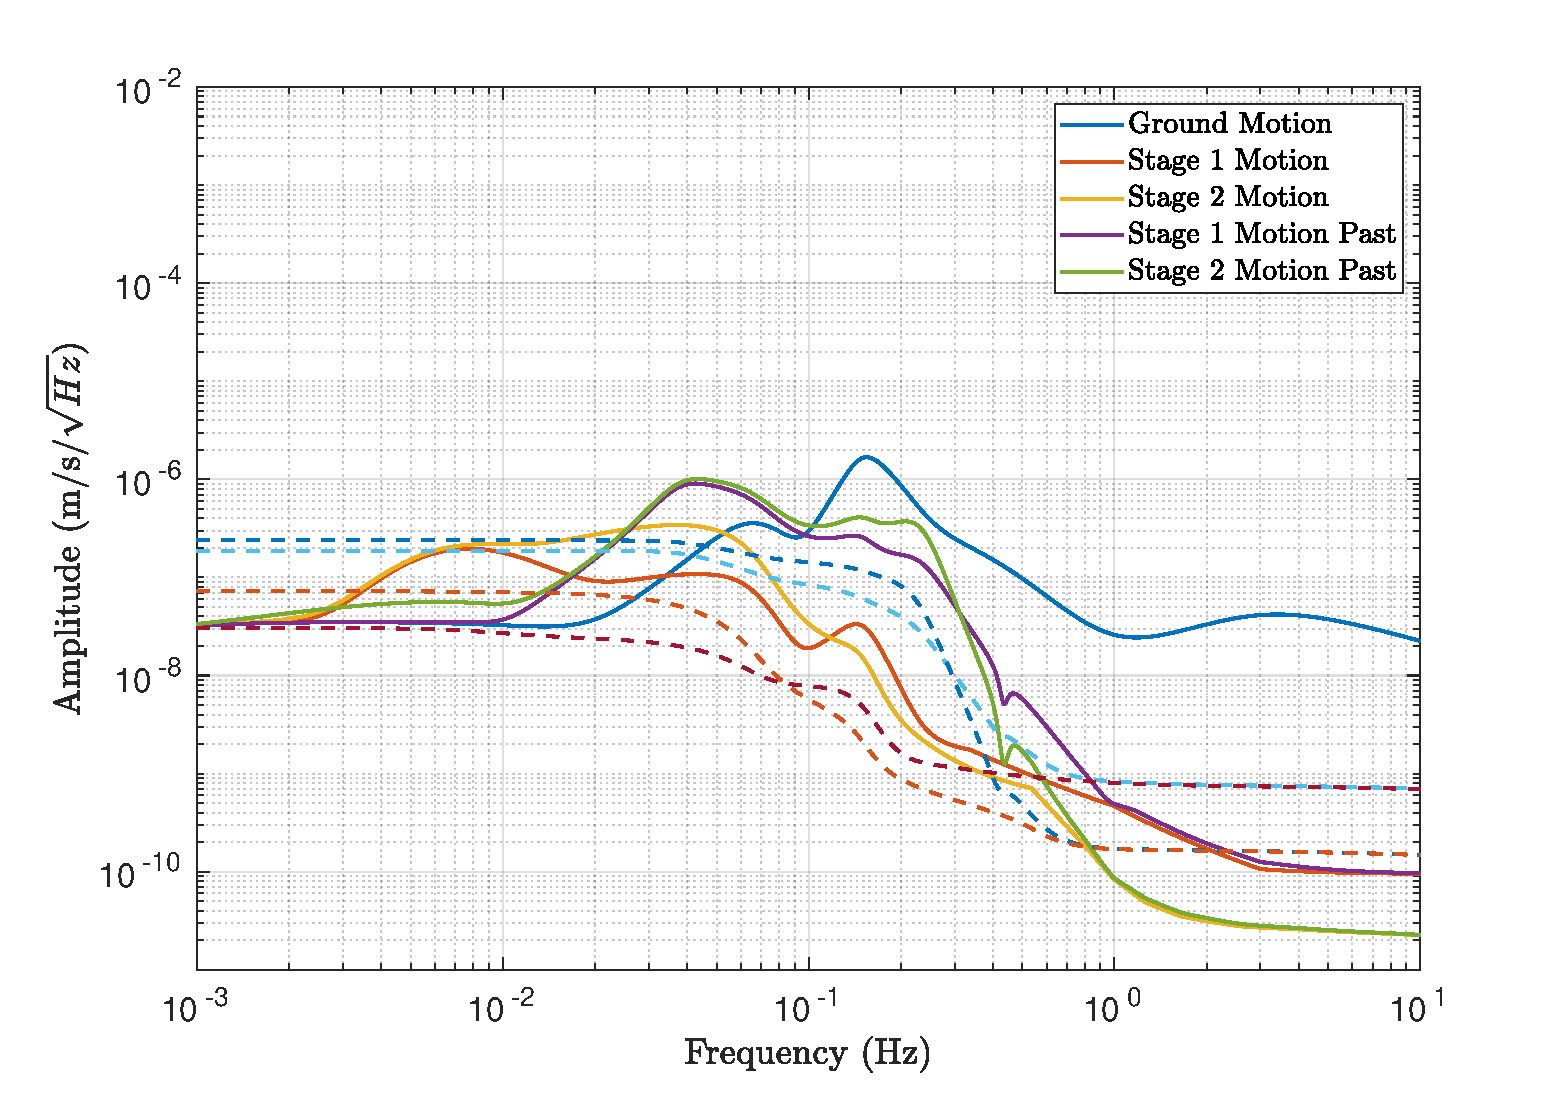
\includegraphics[width=\textwidth]{cBRS_Model_CompX.pdf}
\caption{Comparison of the translational isolation performance during O2 and the projected performance with the inclusion of the cBRS.}
\label{cBRSCompX}
\end{center}
\end{figure}


Although in reality the control loop for each isolation platform will have to be tuned individually, these models show that one can expect a significant decrease in residual motion with the deployment of the cBRS.

\subsection{Angular Control Performance}

\begin{figure}
\begin{center}
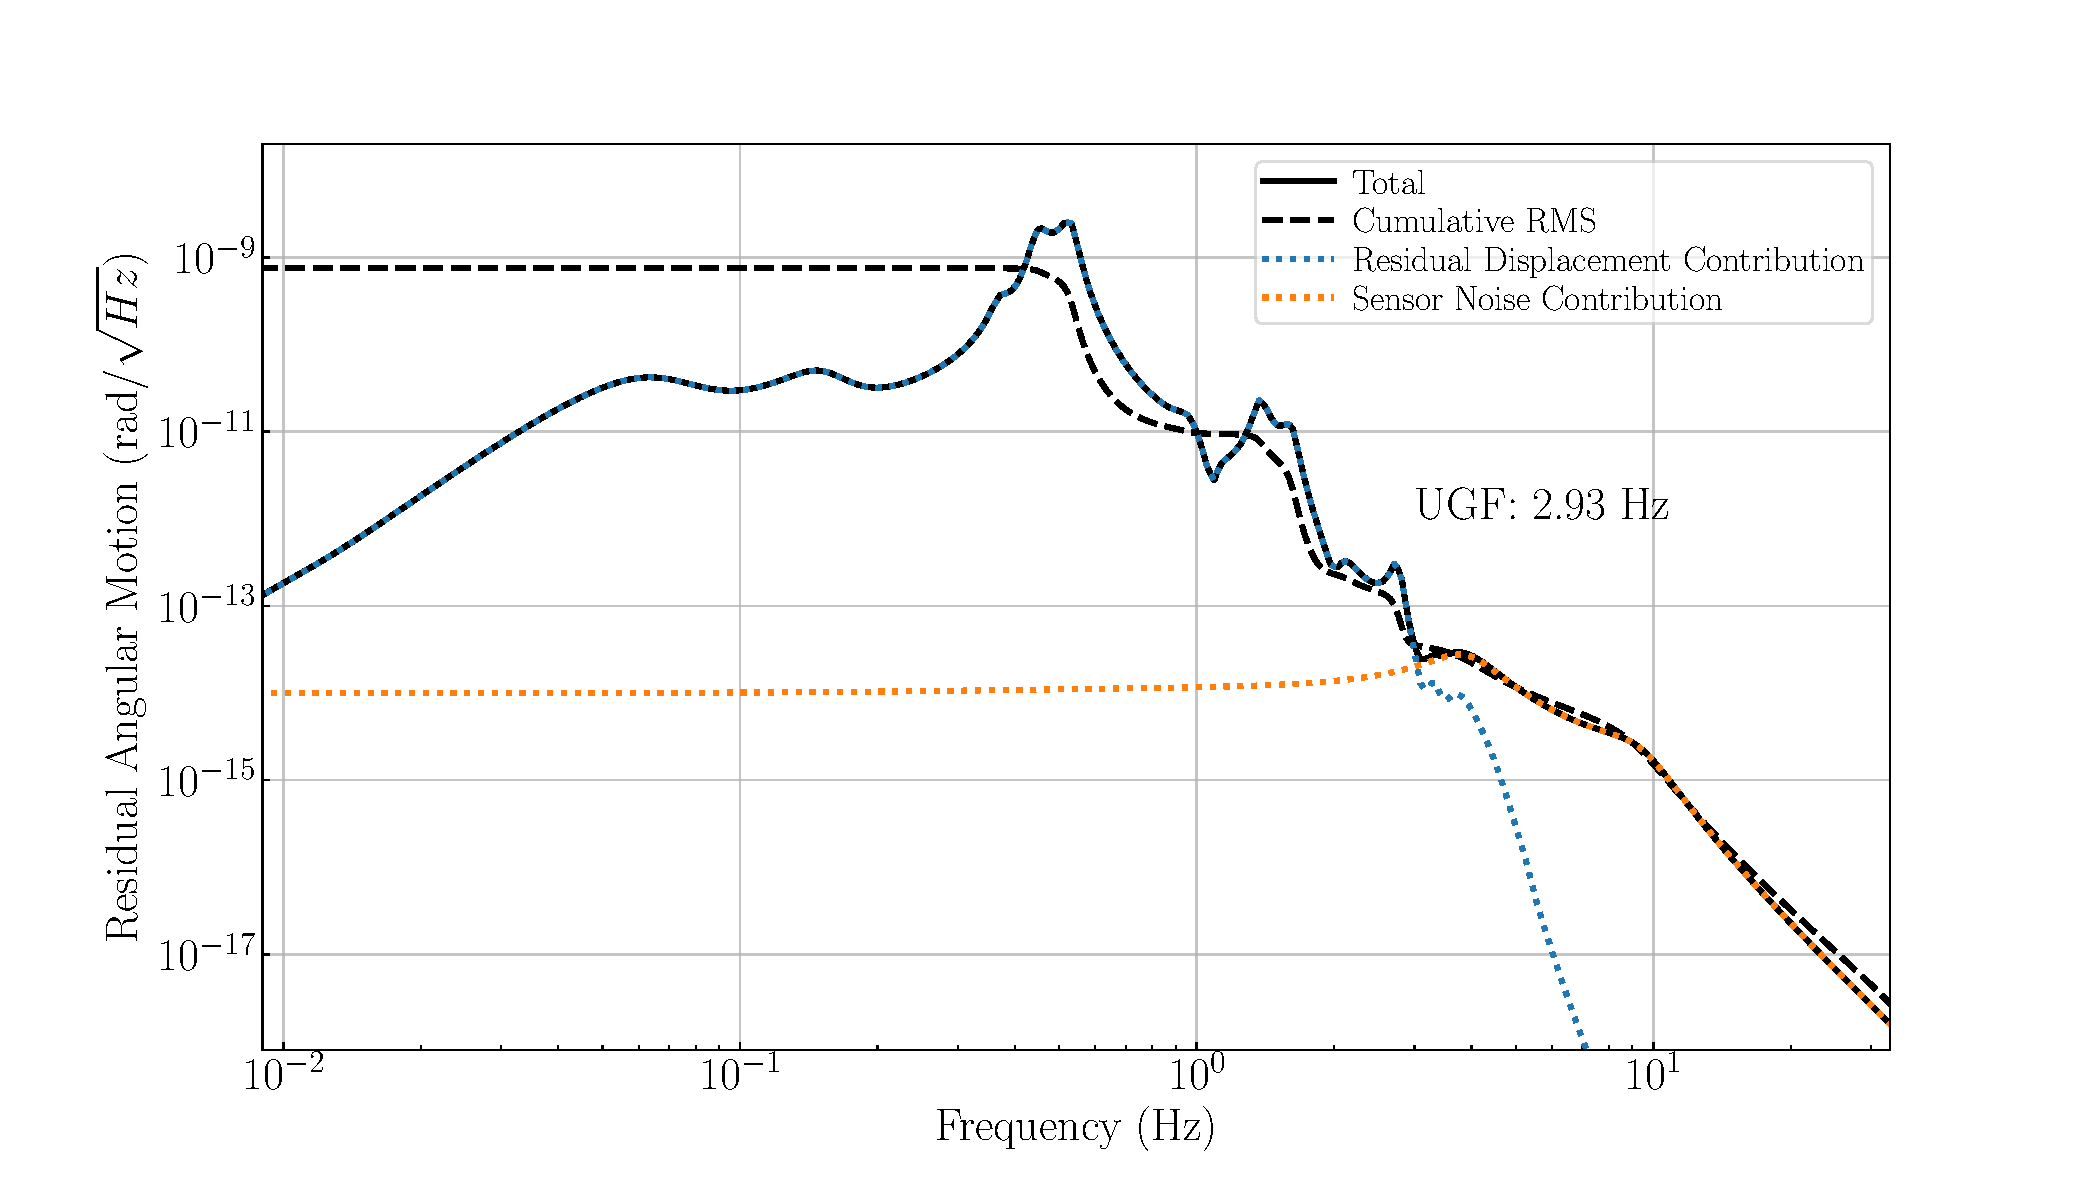
\includegraphics[width=\textwidth]{cBRS_ASC_With.pdf}
\caption{Projected performance of the angular sensing and control system with the seismic performance described in Section \ref{IsoScheme}.}
\label{ascWith}
\end{center}
\end{figure}

\begin{figure}
\begin{center}
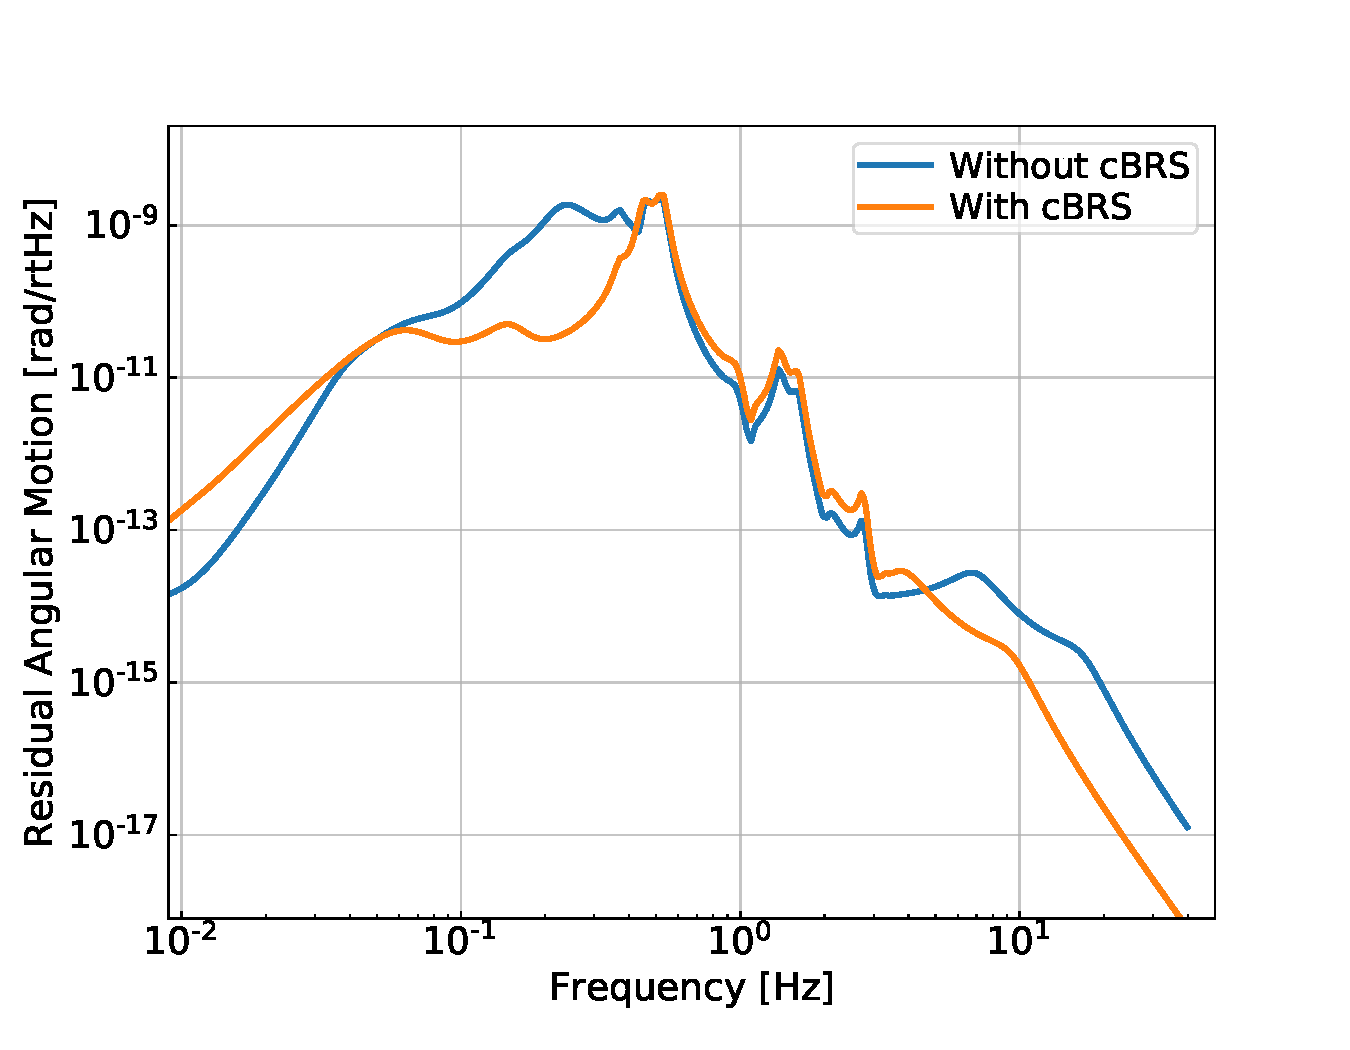
\includegraphics[width=\textwidth]{cBRS_ASC_LowF.pdf}
\caption{Projected performance of the angular sensing and control system with the seismic performance described in Section \ref{IsoScheme}.}
\label{ascComp}
\end{center}
\end{figure}

\begin{figure}
\begin{center}
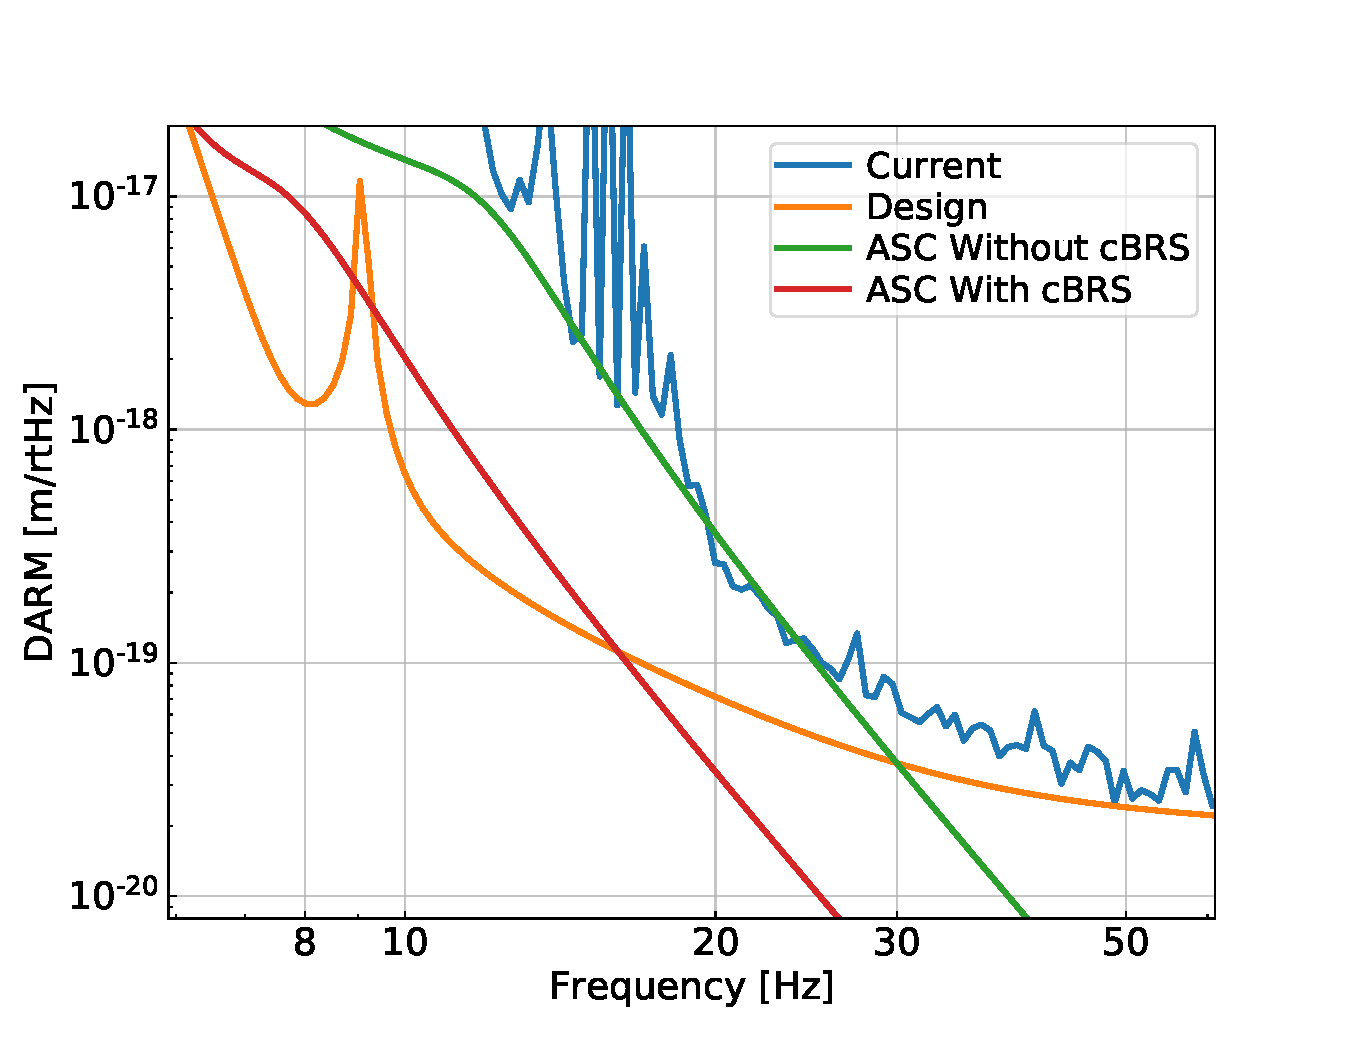
\includegraphics[width=\textwidth]{cBRS_ASC.pdf}
\caption{Projected low frequency strain noise with and without the cBRS. The blue line is the current sensitivity of LLO, the orange is the aLIGO design sensitivity, green is the modeled noise contribution of the current ASC system, and red is the improved ASC noise contribution with the seismic isolation described in Section \ref{IsoScheme}. }
\label{ascStrain}
\end{center}
\end{figure}

\chapter{Applications}
\quad The development of these highly sensitive rotation sensors have opened up a few novel scientific avenues, tangential to seismic isolation, that have been explored and many that have not.

\section{Geophysics}
Seismic waves have six components, three translations and three rotations, however seismology has long neglected the rotational components due the lack of sensitive rotation sensors. Recent developments have begun to alleviated this issue with the advent of seismically relevant ring laser gyros. \cite{ring} The rotation sensors described in Chapter \ref{BRS_chap} and \ref{cBRS_chap} join a small class of ground rotation sensors with that are sensitive enough at low frequencies and have low translational coupling to allow for the use in seismology.
\subsection{Rayleigh Wave Theory}

Seismic waves can be broken into two classes: body waves and surface waves. In regard to surface waves there are two polarization: Love waves and Rayleigh waves. The motion caused by a Love wave is constrained to the plane parallel with the surface of the medium while Rayleigh waves are constrained to a plane perpendicular the surface. 

The plane wave solution of a Rayleigh wave has six components ($u_x, u_y, u_z, \theta_x, \theta_y, \theta_z$) where $u_i$ designated the translational motion in the $i$th direction while $\theta_i$ is the rotation about the $i$th axis.
These can be described as with the following \cite{seismic}
\begin{align}
u_x({\bf r} ,t)&=\alpha \sin(\zeta) \cos(\phi) \cos(\omega t-{\bf k}\cdot{\bf r})\label{XEq}\\
u_y({\bf r} ,t)&=\alpha \sin(\zeta) \sin(\phi) \cos(\omega t-{\bf k}\cdot{\bf r})\\
u_z({\bf r} ,t)&=\alpha \cos(\zeta) \cos(\omega t-{\bf k}\cdot{\bf r}+\pi/2)\label{ZEq}\\
\notag \\
\theta_x({\bf r} ,t)&=\frac{\partial u_z}{\partial y}=\alpha \kappa \cos(\zeta) \sin(\phi) \cos(\omega t-{\bf k}\cdot{\bf r})\label{TiltXEq}\\
\theta_y({\bf r} ,t)&=-\frac{\partial u_z}{\partial x}=-\alpha \kappa \cos(\zeta) \cos(\phi) \cos(\omega t-{\bf k}\cdot{\bf r})\\
\theta_z({\bf r} ,t)&=\frac{1}{2}\Big(\frac{\partial u_y}{\partial x}-\frac{\partial u_x}{\partial y}\Big)=0
\end{align}

where $\alpha$ is the amplitude, $\zeta$ is the ellipticity angle, $\phi$ is the angle of incidence in the horizontal plane, $\omega$ is the frequency, and $\bf{k}=\kappa (\cos(\phi),\sin(\phi),\text{0})$ is the wavevector.

These components can be seen in Figure \ref{Earthquake} which shows the seismic waves sourced by a M 7.9 earthquake in Papua New Guinea as seen by instruments installed at the Y-End station of the LHO. The translations were measured by a broadband three-component seismometer while the rotation was sensed by a Beam Rotation Sensor (BRS) described in Chapter \ref{BRS_chap}. As one would expect from Eq. \ref{ZEq} and \ref{TiltXEq}, the vertical velocity and the rotation differ only by a constant factor related to the phase velocity and the angle of incidence. Additionally, a large amplitude Love wave is apparent starting at $\sim$ 1200 seconds which neither the vertical seismometer or the BRS experiences due to the waves' lack of vertical component.

\begin{figure}%
\begin{center}
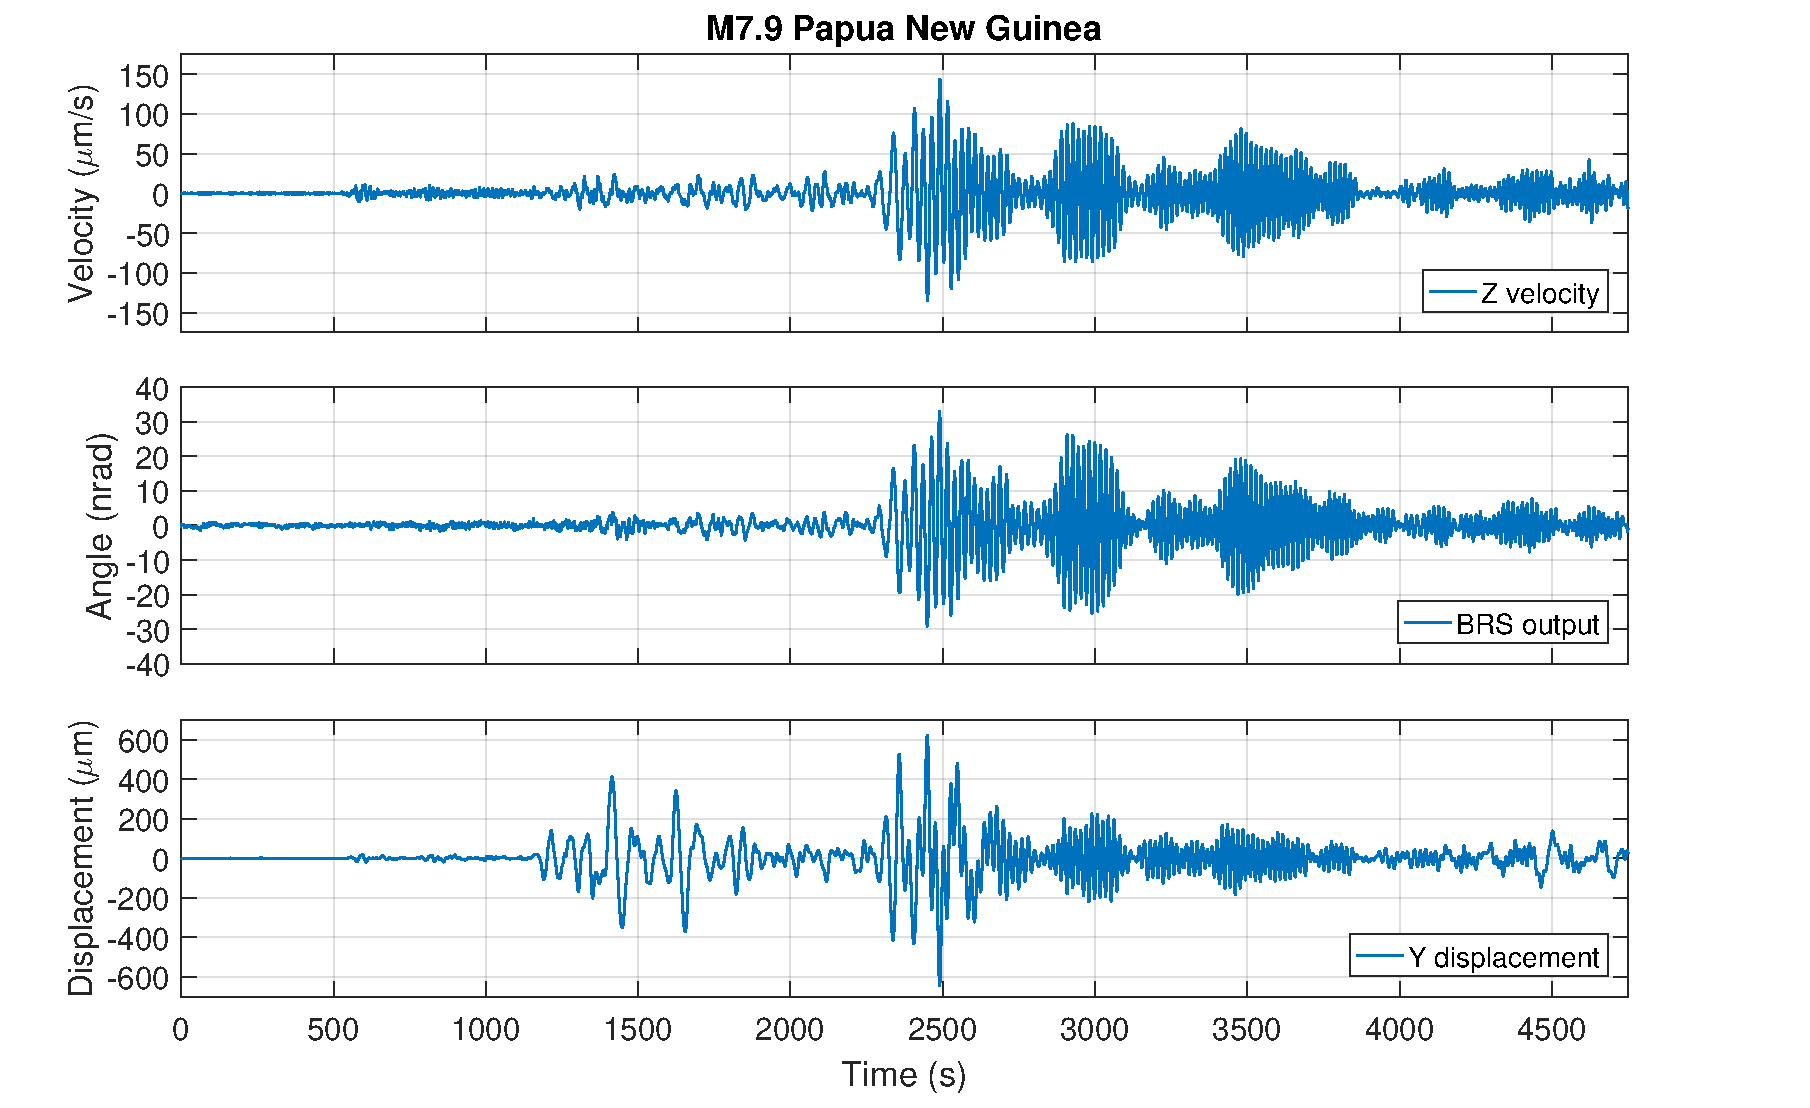
\includegraphics[width=\textwidth]{PNGTimeSeries.pdf}
\caption{Observations of the seismic waves emanated from a M7.9 earthquake in Papua New Guinea as seen by instruments installed at the Y-End Station of LHO. \cite{tiltSeismology} Both the Z velocity and Y displacement were measured by a broadband three-component seismometer while the rotation was measured by a BRS described in Chapter \ref{BRS_chap}. }
\label{Earthquake}
\end{center}
\end{figure}

From these equations it can be seen that with a traditional 3-axis seismometer, one can not measure all five parameters that define this wave-field. Additionally, the horizontal components, $u_x\text{ and }u_y$ can contain contributions from co-propagating Love waves which further muddles ones ability to extract parameters. 


\subsection{wave-field Parameter Extraction}

With the combined measurements of the translational and rotational components at a single station, one can readily extract wavefield parameters that would otherwise be difficult to obtain, namely the phase velocity and angle of incidence. 

Seismic wave phase velocities are a common observable which not only allows for understanding of Rayleigh wave propogation but can be inverted to yield tomographical structure profiles of the interior of the earth. \textbf{cite} The traditional method of extracting these is by exploiting the time of arrival of a wave as it passes through an array of many seismometers. The analysis can be constrained to only the vertical channel which is insensitive to Love waves which could contaminate the measurements. However, this method requires many devices and effectively averages over the size of the array.

Alternatively, with measurements of the rotational components a point like measurement of the phase velocity can be made with three devices, a 3-component seismometer and two horizontal rotation sensors. This can be shown in the following equations:
\begin{align} 
v&\equiv\frac{\omega}{\kappa} = \frac{\dot{u_z}}{\theta_x}\sin(\phi) \label{vx} \\
v&=\frac{\dot{u_z}}{\theta_y}\cos(\phi)\label{vy} \\
v&=\frac{\dot{u_z}}{\sqrt{\theta_x^2+\theta_y^2}} \label{v}
\end{align}

where the dot represents the temporal derivative. Equations \ref{vx} and \ref{vy} can be utilized if a station has only one horizontal rotation sensor but requires independent determination of $\phi$, the angle of incidence. In contrast, Equation \ref{v} contains only information from a single station.

In addition to the phase velocity, the angle of incidence can be determined with the following:
\begin{align}
\phi=\text{arctan}\bigg(\frac{\theta_x}{\theta_y}\bigg)
\end{align}

Although in theory, this can be measured using a single seismometer, Love wave contamination of the horizontal translational channels would distort any such measurement. As the horizontal rotational channels are insensitive to Love waves, they allow the extraction of $\phi$ without such contamination.  

\subsection{Single Station Dispersion Measurements}
%\subsubsection{Hanford Measurements}
As described in Section \ref{BRS_Hanford}, two BRSs were installed at LHO, one at each end station located 5.66 meters apart. The End-X BRS was found to have a $\delta=30\ \mu \text{m}$ leading to a translational coupling of $2 \times 10^{-4}$ rad/m while the End-Y BRS was found to have a coupling of $1 \times 10^{-6}$ rad/m with a $\delta<0.5\ \mu \text{m}$. This limited any seismic studies using these devices to use only the End-Y BRS as the End-X BRS was contaminated with translational motion. 

Between April, 2016 and January, 2017, six earthquakes were measured during environmentally quite times at the observatory. \cite{tiltSeismology} With application of Eq. \ref{vx} the phase dispersion curve at the Y-End Station was measured with instruments installed at a single station. Corrections of the angle of incidence were determined via an array of seismometers installed at LHO which were verified via great circle calculations. Additionally, the phase velocity was estimated in a more traditional manor using the signal delay between the array of seismometer at LHO. The measure phase dispersion curve is shown in Figure \ref{Phase_Hanford} which shows good agreement between the two methods. For more detail see Reference \cite{TiltSeimology}
 
\begin{figure}%
\begin{center}
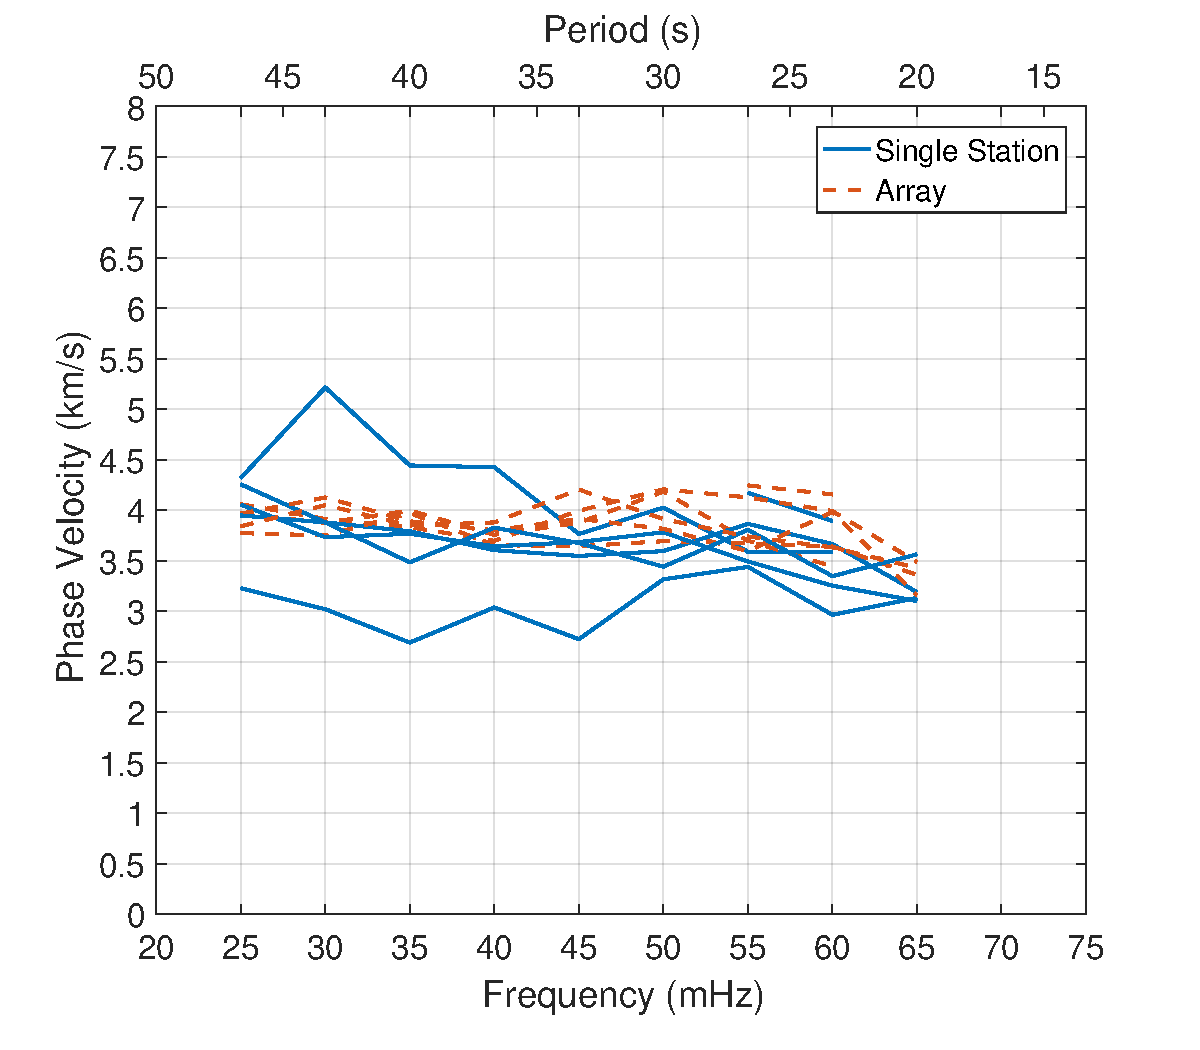
\includegraphics[width=0.75\textwidth]{Vel.pdf}
\caption{Rayleigh wave phase velocity measurements made by instruments located at the End-Y station of LHO, blue, and the same measurements achieved by the array of seismometers deployed at LHO. Each line represent the measurements achieved by different earthquakes. The angle of incidence of each wave was measured independent of the single station and used within the analysis. \cite{tiltSeismology}}
\label{Phase_Hanford}
\end{center}
\end{figure}

These measurements display the utility of including rotation sensors in seismic instruments. If a seismic station was constructed with two orthogonally oriented horizontal rotation sensors and a vertical seismometer, the phase velocity could be measured independent of angle of incidence by utilizing Eq. \ref{v}. Neglecting the logistical difficulty, one could imagine constructing arrays of station with both translational and rotational sensors. This would allow mapping of the phase dispersion curves, and thus tomography, with spatial resolution limited only by the size of the instruments. Such stations could also be installed within traditional arrays to yield independent point like measurements to further constrain tomographic studies.

%\subsubsection{Livingston Measurements}
%
%\begin{figure}%
%\begin{center}
%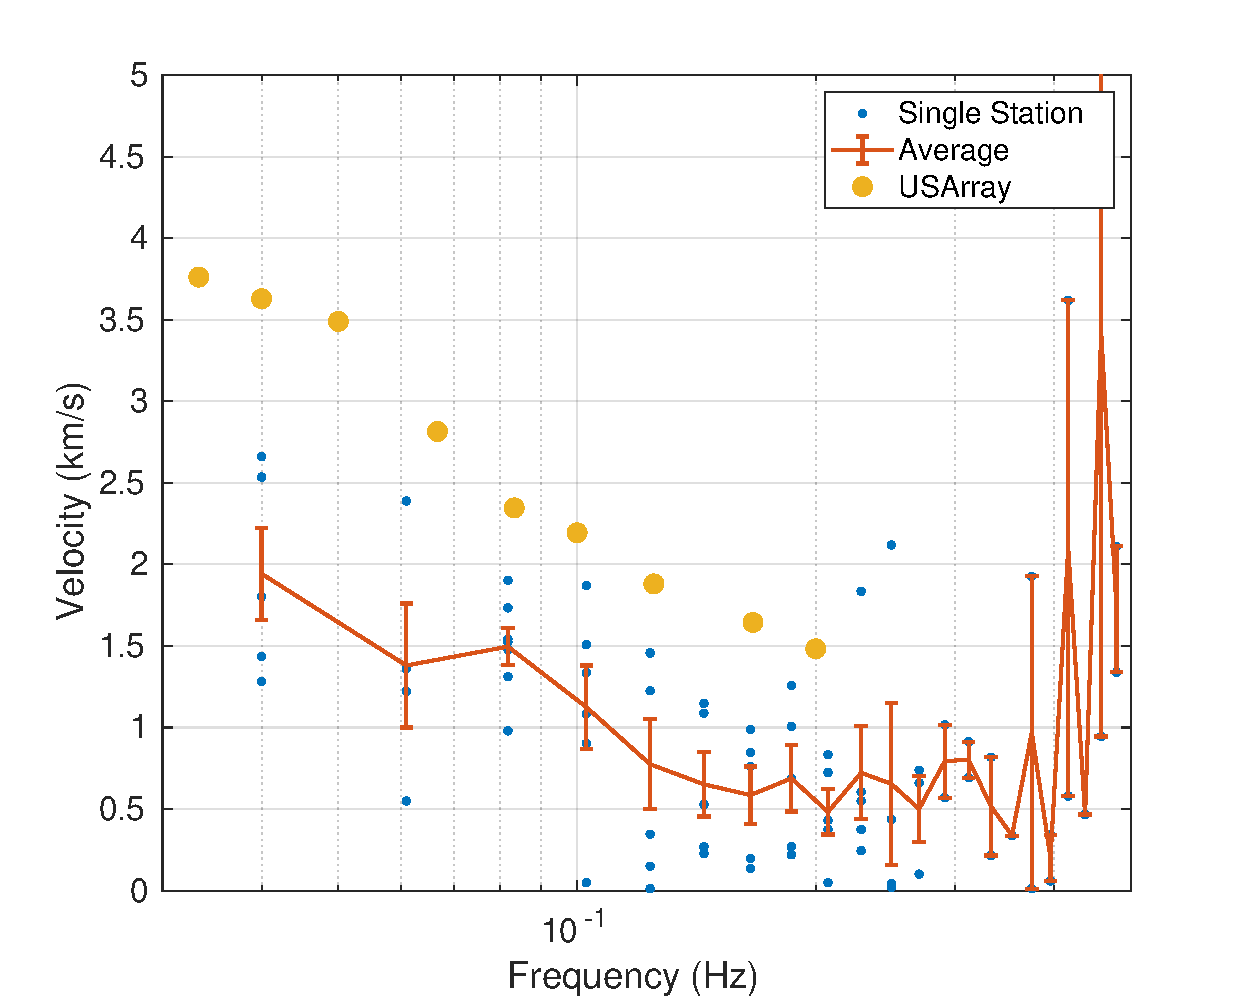
\includegraphics[width=\textwidth]{RayleighDispersion.pdf}
%\caption{True single station Rayleigh wave phase velocity measurements achieved at LLO. The measurements from each earthquake are shown in blue while red shows the average and standard deviation of these measurements. The yellow dots represent measurements made independently by the USArray seismometer array deployment.}
%\label{Phase_Livingston}
%\end{center}
%\end{figure}

\section{Newtonian Noise}
\subsection{Theory}

The gravitational coupling between the environment and an interferometer's test masses, so called Newtonian noise, is expected to limit the performance of terrestrial gravitational wave detectors in the near future \textbf{CITE}. Sources of the gravitaitonal field variations can range from atmospheric density changes to vibrations of the laboratory structures \textbf{CITE}. This coupling is unique in the fact that it can not be shielded or trivially engineered away. One can move an observatory underground to decrease the strength of the atmospherically driven fluctuations and those caused by seismic surface waves, discussed in detail in the following section. However, this process is both expensive and does not remove the sources which come from operating an instrument such as the vibrations of the vacuum structure or seismic motion sourced by laboratory equipment. 

For the current surface-level interferometric observatories, the seismic motion due to Rayleigh waves is thought to be the dominant contributor to the Newtonian noise and will be the limiting noise source between \textbf{5-30 Hz} \cite{}. The motion due to a plane Rayleigh wave follows:

\begin{equation}
u_z({\bf r} ,t)=u_z \cos(\omega t-{\bf k}\cdot{\bf r}+\pi/2) \label{uz}
\end{equation}

where $u_z=\alpha \cos(\zeta)$, $\alpha$ is the amplitude, $\zeta$ is the ellipticity angle, $\phi$ is the angle of incidence in the horizontal plane, $\omega$ is the frequency, and $\bf{k}=\kappa (\cos(\phi),\sin(\phi),\text{0})$ is the wavevector. The corresponding test mass acceleration in the x-direction follows \cite{Harms_2016}:
\begin{equation}
a_x({\bf r} ,t)=2 \pi u_z \gamma G \rho_0 e^{-h \kappa}  \cos(\phi) \cos(\omega t-{\bf k}\cdot{\bf r}) \label{a}
\end{equation}
where $G$ is the gravitational constant, $\rho_0$ is the density of the ground, $h$ is the height of the test mass from the ground, and $\gamma \approx 0.8$ is a factor which accounts for the counter-action of the change of density due to the seismic wave and the vertical motion of the ground.

At first glance, these equations appear to suggest that one could predict the test mass acceleration for a given vertical seismometer signal. Such a prediction would allow for high quality subtraction of the Newtonian Noise from an observatories data stream. However, true seismic wave-fields are not composed of stationary Rayleigh waves but instead are comprised of the sum of many desperate sources which may change their amplitude and phase in time. With this consideration, the phase difference between Eq. \ref{uz} and \ref{a} and the lack of angle of incidence dependence in Eq. \ref{uz} destroy the ability to use a single vertical seismometer as a reliable sensor for Newtonian noise subtraction.

On the other hand, a horizontal seismometer described by Eq. \ref{XEq} is both in phase with the Newtonian noise signal and has the same angular dependence. However, seismic wave-fields also include Love waves which have horizontal components but no vertical. This contaminates these channels and would decrease the correlation between the horizontal seismometer and the Newtonian noise. 

Finally, the tilt, being the rotation about the y-axis, due to a Rayleigh wave is described by the following:

\begin{equation}
\theta_y({\bf r} ,t)=\frac{\partial u_z}{\partial x}=u_z \kappa \cos(\phi) \cos(\omega t-{\bf k}\cdot{\bf r})\label{tX}\\
\end{equation}

The tilt is thus both in phase, has the same angular dependence, and does not include Love waves. The lack of Love waves can be seen in Figure \ref{Earthquake} when the horizontal seismometer experiences a large Love wave at around \textbf{1000 s} while the rotation sensor sees no such signal. The tilt signal and the Newtonian noise are thus related by a handful of parameters which can be measured independently or determined empirically and are not expected to vary in time. This points to the conclusion that a tiltmeter is the ideal sensor for Newtonian noise subtraction

\subsection{Observations}

\textbf{cBRS installed at Hanford}

\textbf{array subtraction}

\textbf{location due to size}

\textbf{tilt to h(t) coupling}

\printendnotes
\nocite{*}   
\bibliographystyle{plain}
\bibliography{Dissertation}
\end{document}


